% Options for packages loaded elsewhere
\PassOptionsToPackage{unicode}{hyperref}
\PassOptionsToPackage{hyphens}{url}
%
\documentclass[
]{article}
\usepackage{amsmath,amssymb}
\usepackage{iftex}
\ifPDFTeX
  \usepackage[T1]{fontenc}
  \usepackage[utf8]{inputenc}
  \usepackage{textcomp} % provide euro and other symbols
\else % if luatex or xetex
  \usepackage{unicode-math} % this also loads fontspec
  \defaultfontfeatures{Scale=MatchLowercase}
  \defaultfontfeatures[\rmfamily]{Ligatures=TeX,Scale=1}
\fi
\usepackage{lmodern}
\ifPDFTeX\else
  % xetex/luatex font selection
\fi
% Use upquote if available, for straight quotes in verbatim environments
\IfFileExists{upquote.sty}{\usepackage{upquote}}{}
\IfFileExists{microtype.sty}{% use microtype if available
  \usepackage[]{microtype}
  \UseMicrotypeSet[protrusion]{basicmath} % disable protrusion for tt fonts
}{}
\makeatletter
\@ifundefined{KOMAClassName}{% if non-KOMA class
  \IfFileExists{parskip.sty}{%
    \usepackage{parskip}
  }{% else
    \setlength{\parindent}{0pt}
    \setlength{\parskip}{6pt plus 2pt minus 1pt}}
}{% if KOMA class
  \KOMAoptions{parskip=half}}
\makeatother
\usepackage{xcolor}
\usepackage[margin=1in]{geometry}
\usepackage{color}
\usepackage{fancyvrb}
\newcommand{\VerbBar}{|}
\newcommand{\VERB}{\Verb[commandchars=\\\{\}]}
\DefineVerbatimEnvironment{Highlighting}{Verbatim}{commandchars=\\\{\}}
% Add ',fontsize=\small' for more characters per line
\usepackage{framed}
\definecolor{shadecolor}{RGB}{248,248,248}
\newenvironment{Shaded}{\begin{snugshade}}{\end{snugshade}}
\newcommand{\AlertTok}[1]{\textcolor[rgb]{0.94,0.16,0.16}{#1}}
\newcommand{\AnnotationTok}[1]{\textcolor[rgb]{0.56,0.35,0.01}{\textbf{\textit{#1}}}}
\newcommand{\AttributeTok}[1]{\textcolor[rgb]{0.13,0.29,0.53}{#1}}
\newcommand{\BaseNTok}[1]{\textcolor[rgb]{0.00,0.00,0.81}{#1}}
\newcommand{\BuiltInTok}[1]{#1}
\newcommand{\CharTok}[1]{\textcolor[rgb]{0.31,0.60,0.02}{#1}}
\newcommand{\CommentTok}[1]{\textcolor[rgb]{0.56,0.35,0.01}{\textit{#1}}}
\newcommand{\CommentVarTok}[1]{\textcolor[rgb]{0.56,0.35,0.01}{\textbf{\textit{#1}}}}
\newcommand{\ConstantTok}[1]{\textcolor[rgb]{0.56,0.35,0.01}{#1}}
\newcommand{\ControlFlowTok}[1]{\textcolor[rgb]{0.13,0.29,0.53}{\textbf{#1}}}
\newcommand{\DataTypeTok}[1]{\textcolor[rgb]{0.13,0.29,0.53}{#1}}
\newcommand{\DecValTok}[1]{\textcolor[rgb]{0.00,0.00,0.81}{#1}}
\newcommand{\DocumentationTok}[1]{\textcolor[rgb]{0.56,0.35,0.01}{\textbf{\textit{#1}}}}
\newcommand{\ErrorTok}[1]{\textcolor[rgb]{0.64,0.00,0.00}{\textbf{#1}}}
\newcommand{\ExtensionTok}[1]{#1}
\newcommand{\FloatTok}[1]{\textcolor[rgb]{0.00,0.00,0.81}{#1}}
\newcommand{\FunctionTok}[1]{\textcolor[rgb]{0.13,0.29,0.53}{\textbf{#1}}}
\newcommand{\ImportTok}[1]{#1}
\newcommand{\InformationTok}[1]{\textcolor[rgb]{0.56,0.35,0.01}{\textbf{\textit{#1}}}}
\newcommand{\KeywordTok}[1]{\textcolor[rgb]{0.13,0.29,0.53}{\textbf{#1}}}
\newcommand{\NormalTok}[1]{#1}
\newcommand{\OperatorTok}[1]{\textcolor[rgb]{0.81,0.36,0.00}{\textbf{#1}}}
\newcommand{\OtherTok}[1]{\textcolor[rgb]{0.56,0.35,0.01}{#1}}
\newcommand{\PreprocessorTok}[1]{\textcolor[rgb]{0.56,0.35,0.01}{\textit{#1}}}
\newcommand{\RegionMarkerTok}[1]{#1}
\newcommand{\SpecialCharTok}[1]{\textcolor[rgb]{0.81,0.36,0.00}{\textbf{#1}}}
\newcommand{\SpecialStringTok}[1]{\textcolor[rgb]{0.31,0.60,0.02}{#1}}
\newcommand{\StringTok}[1]{\textcolor[rgb]{0.31,0.60,0.02}{#1}}
\newcommand{\VariableTok}[1]{\textcolor[rgb]{0.00,0.00,0.00}{#1}}
\newcommand{\VerbatimStringTok}[1]{\textcolor[rgb]{0.31,0.60,0.02}{#1}}
\newcommand{\WarningTok}[1]{\textcolor[rgb]{0.56,0.35,0.01}{\textbf{\textit{#1}}}}
\usepackage{graphicx}
\makeatletter
\def\maxwidth{\ifdim\Gin@nat@width>\linewidth\linewidth\else\Gin@nat@width\fi}
\def\maxheight{\ifdim\Gin@nat@height>\textheight\textheight\else\Gin@nat@height\fi}
\makeatother
% Scale images if necessary, so that they will not overflow the page
% margins by default, and it is still possible to overwrite the defaults
% using explicit options in \includegraphics[width, height, ...]{}
\setkeys{Gin}{width=\maxwidth,height=\maxheight,keepaspectratio}
% Set default figure placement to htbp
\makeatletter
\def\fps@figure{htbp}
\makeatother
\setlength{\emergencystretch}{3em} % prevent overfull lines
\providecommand{\tightlist}{%
  \setlength{\itemsep}{0pt}\setlength{\parskip}{0pt}}
\setcounter{secnumdepth}{-\maxdimen} % remove section numbering
\ifLuaTeX
  \usepackage{selnolig}  % disable illegal ligatures
\fi
\usepackage{bookmark}
\IfFileExists{xurl.sty}{\usepackage{xurl}}{} % add URL line breaks if available
\urlstyle{same}
\hypersetup{
  pdftitle={R\_Assignment},
  pdfauthor={Zheyuan Zhang},
  hidelinks,
  pdfcreator={LaTeX via pandoc}}

\title{R\_Assignment}
\author{Zheyuan Zhang}
\date{3/14/2025}

\begin{document}
\maketitle

\subsection{Part I}\label{part-i}

\subsubsection{Data Inspection}\label{data-inspection}

\paragraph{Check the enviomental
frame}\label{check-the-enviomental-frame}

\begin{Shaded}
\begin{Highlighting}[]
\FunctionTok{library}\NormalTok{(}\StringTok{"tidyverse"}\NormalTok{)}
\end{Highlighting}
\end{Shaded}

\begin{verbatim}
## -- Attaching core tidyverse packages ------------------------ tidyverse 2.0.0 --
## v dplyr     1.1.4     v readr     2.1.5
## v forcats   1.0.0     v stringr   1.5.1
## v ggplot2   3.5.1     v tibble    3.2.1
## v lubridate 1.9.3     v tidyr     1.3.1
## v purrr     1.0.2     
## -- Conflicts ------------------------------------------ tidyverse_conflicts() --
## x dplyr::filter() masks stats::filter()
## x dplyr::lag()    masks stats::lag()
## i Use the conflicted package (<http://conflicted.r-lib.org/>) to force all conflicts to become errors
\end{verbatim}

\begin{Shaded}
\begin{Highlighting}[]
\FunctionTok{library}\NormalTok{(ggplot2)}
\end{Highlighting}
\end{Shaded}

\paragraph{Read files}\label{read-files}

\begin{Shaded}
\begin{Highlighting}[]
\NormalTok{raw\_genotypes }\OtherTok{\textless{}{-}} \FunctionTok{read\_tsv}\NormalTok{(}\StringTok{"fang\_et\_al\_genotypes.txt"}\NormalTok{)}
\end{Highlighting}
\end{Shaded}

\begin{verbatim}
## Rows: 2782 Columns: 986
## -- Column specification --------------------------------------------------------
## Delimiter: "\t"
## chr (986): Sample_ID, JG_OTU, Group, abph1.20, abph1.22, ae1.3, ae1.4, ae1.5...
## 
## i Use `spec()` to retrieve the full column specification for this data.
## i Specify the column types or set `show_col_types = FALSE` to quiet this message.
\end{verbatim}

\begin{Shaded}
\begin{Highlighting}[]
\NormalTok{raw\_snp\_position }\OtherTok{\textless{}{-}} \FunctionTok{read\_tsv}\NormalTok{(}\StringTok{"snp\_position.txt"}\NormalTok{)}
\end{Highlighting}
\end{Shaded}

\begin{verbatim}
## Rows: 983 Columns: 15
## -- Column specification --------------------------------------------------------
## Delimiter: "\t"
## chr (9): SNP_ID, Chromosome, Position, alt_pos, mult_positions, amplicon, cd...
## dbl (6): cdv_marker_id, Genaissance_daa_id, Sequenom_daa_id, count_amplicons...
## 
## i Use `spec()` to retrieve the full column specification for this data.
## i Specify the column types or set `show_col_types = FALSE` to quiet this message.
\end{verbatim}

\paragraph{Inspect:}\label{inspect}

\begin{Shaded}
\begin{Highlighting}[]
\FunctionTok{head}\NormalTok{(raw\_genotypes)}
\end{Highlighting}
\end{Shaded}

\begin{verbatim}
## # A tibble: 6 x 986
##   Sample_ID JG_OTU   Group abph1.20 abph1.22 ae1.3 ae1.4 ae1.5 an1.4 ba1.6 ba1.9
##   <chr>     <chr>    <chr> <chr>    <chr>    <chr> <chr> <chr> <chr> <chr> <chr>
## 1 SL-15     T-aust-1 TRIPS ?/?      ?/?      T/T   G/G   T/T   C/C   ?/?   G/G  
## 2 SL-16     T-aust-2 TRIPS ?/?      ?/?      T/T   ?/?   T/T   C/C   A/G   G/G  
## 3 SL-11     T-brav-1 TRIPS ?/?      ?/?      T/T   G/G   T/T   ?/?   G/G   G/G  
## 4 SL-12     T-brav-2 TRIPS ?/?      ?/?      T/T   G/G   T/T   C/C   G/G   G/G  
## 5 SL-18     T-cund   TRIPS ?/?      ?/?      T/T   G/G   T/T   C/C   ?/?   G/G  
## 6 SL-2      T-dact-1 TRIPS ?/?      ?/?      T/T   G/G   T/T   C/C   A/G   G/G  
## # i 975 more variables: bt2.5 <chr>, bt2.7 <chr>, bt2.8 <chr>, Fea2.1 <chr>,
## #   Fea2.5 <chr>, id1.3 <chr>, lg2.11 <chr>, lg2.2 <chr>, pbf1.1 <chr>,
## #   pbf1.2 <chr>, pbf1.3 <chr>, pbf1.5 <chr>, pbf1.6 <chr>, pbf1.7 <chr>,
## #   pbf1.8 <chr>, PZA00003.11 <chr>, PZA00004.2 <chr>, PZA00005.8 <chr>,
## #   PZA00005.9 <chr>, PZA00006.13 <chr>, PZA00006.14 <chr>, PZA00008.1 <chr>,
## #   PZA00010.5 <chr>, PZA00013.10 <chr>, PZA00013.11 <chr>, PZA00013.9 <chr>,
## #   PZA00015.4 <chr>, PZA00017.1 <chr>, PZA00018.5 <chr>, ...
\end{verbatim}

\begin{Shaded}
\begin{Highlighting}[]
\FunctionTok{head}\NormalTok{(raw\_snp\_position)}
\end{Highlighting}
\end{Shaded}

\begin{verbatim}
## # A tibble: 6 x 15
##   SNP_ID   cdv_marker_id Chromosome Position  alt_pos mult_positions amplicon
##   <chr>            <dbl> <chr>      <chr>     <chr>   <chr>          <chr>   
## 1 abph1.20          5976 2          27403404  <NA>    <NA>           abph1   
## 2 abph1.22          5978 2          27403892  <NA>    <NA>           abph1   
## 3 ae1.3             6605 5          167889790 <NA>    <NA>           ae1     
## 4 ae1.4             6606 5          167889682 <NA>    <NA>           ae1     
## 5 ae1.5             6607 5          167889821 <NA>    <NA>           ae1     
## 6 an1.4             5982 1          240498509 <NA>    <NA>           an1     
## # i 8 more variables: cdv_map_feature.name <chr>, gene <chr>,
## #   `candidate/random` <chr>, Genaissance_daa_id <dbl>, Sequenom_daa_id <dbl>,
## #   count_amplicons <dbl>, count_cmf <dbl>, count_gene <dbl>
\end{verbatim}

\begin{Shaded}
\begin{Highlighting}[]
\FunctionTok{dim}\NormalTok{(raw\_genotypes)}
\end{Highlighting}
\end{Shaded}

\begin{verbatim}
## [1] 2782  986
\end{verbatim}

\begin{Shaded}
\begin{Highlighting}[]
\FunctionTok{dim}\NormalTok{(raw\_snp\_position)}
\end{Highlighting}
\end{Shaded}

\begin{verbatim}
## [1] 983  15
\end{verbatim}

\begin{Shaded}
\begin{Highlighting}[]
\FunctionTok{str}\NormalTok{(raw\_genotypes)}
\end{Highlighting}
\end{Shaded}

\begin{verbatim}
## spc_tbl_ [2,782 x 986] (S3: spec_tbl_df/tbl_df/tbl/data.frame)
##  $ Sample_ID     : chr [1:2782] "SL-15" "SL-16" "SL-11" "SL-12" ...
##  $ JG_OTU        : chr [1:2782] "T-aust-1" "T-aust-2" "T-brav-1" "T-brav-2" ...
##  $ Group         : chr [1:2782] "TRIPS" "TRIPS" "TRIPS" "TRIPS" ...
##  $ abph1.20      : chr [1:2782] "?/?" "?/?" "?/?" "?/?" ...
##  $ abph1.22      : chr [1:2782] "?/?" "?/?" "?/?" "?/?" ...
##  $ ae1.3         : chr [1:2782] "T/T" "T/T" "T/T" "T/T" ...
##  $ ae1.4         : chr [1:2782] "G/G" "?/?" "G/G" "G/G" ...
##  $ ae1.5         : chr [1:2782] "T/T" "T/T" "T/T" "T/T" ...
##  $ an1.4         : chr [1:2782] "C/C" "C/C" "?/?" "C/C" ...
##  $ ba1.6         : chr [1:2782] "?/?" "A/G" "G/G" "G/G" ...
##  $ ba1.9         : chr [1:2782] "G/G" "G/G" "G/G" "G/G" ...
##  $ bt2.5         : chr [1:2782] "?/?" "?/?" "C/C" "C/C" ...
##  $ bt2.7         : chr [1:2782] "A/A" "A/A" "A/A" "A/A" ...
##  $ bt2.8         : chr [1:2782] "?/?" "?/?" "?/?" "?/?" ...
##  $ Fea2.1        : chr [1:2782] "C/C" "C/C" "?/?" "?/?" ...
##  $ Fea2.5        : chr [1:2782] "A/A" "A/A" "A/A" "A/A" ...
##  $ id1.3         : chr [1:2782] "T/T" "T/T" "T/T" "T/T" ...
##  $ lg2.11        : chr [1:2782] "C/C" "C/C" "C/C" "C/C" ...
##  $ lg2.2         : chr [1:2782] "A/A" "A/A" "A/A" "A/A" ...
##  $ pbf1.1        : chr [1:2782] "?/?" "T/T" "T/T" "T/T" ...
##  $ pbf1.2        : chr [1:2782] "?/?" "?/?" "?/?" "?/?" ...
##  $ pbf1.3        : chr [1:2782] "?/?" "?/?" "?/?" "?/?" ...
##  $ pbf1.5        : chr [1:2782] "?/?" "?/?" "A/A" "A/A" ...
##  $ pbf1.6        : chr [1:2782] "?/?" "?/?" "?/?" "?/?" ...
##  $ pbf1.7        : chr [1:2782] "C/C" "C/C" "C/C" "C/C" ...
##  $ pbf1.8        : chr [1:2782] "C/C" "C/C" "C/C" "C/C" ...
##  $ PZA00003.11   : chr [1:2782] "?/?" "?/?" "C/C" "?/?" ...
##  $ PZA00004.2    : chr [1:2782] "T/T" "T/T" "?/?" "T/T" ...
##  $ PZA00005.8    : chr [1:2782] "G/G" "G/G" "G/G" "G/G" ...
##  $ PZA00005.9    : chr [1:2782] "C/C" "C/C" "C/C" "C/C" ...
##  $ PZA00006.13   : chr [1:2782] "A/A" "A/A" "A/A" "A/A" ...
##  $ PZA00006.14   : chr [1:2782] "?/?" "G/G" "G/G" "G/G" ...
##  $ PZA00008.1    : chr [1:2782] "C/C" "C/C" "C/C" "C/C" ...
##  $ PZA00010.5    : chr [1:2782] "C/C" "C/C" "C/C" "C/C" ...
##  $ PZA00013.10   : chr [1:2782] "A/A" "A/A" "A/A" "A/A" ...
##  $ PZA00013.11   : chr [1:2782] "C/C" "C/C" "C/T" "C/T" ...
##  $ PZA00013.9    : chr [1:2782] "T/T" "T/T" "T/T" "T/T" ...
##  $ PZA00015.4    : chr [1:2782] "?/?" "?/?" "?/?" "?/?" ...
##  $ PZA00017.1    : chr [1:2782] "G/G" "G/G" "G/G" "G/G" ...
##  $ PZA00018.5    : chr [1:2782] "C/C" "C/C" "C/C" "C/C" ...
##  $ PZA00029.11   : chr [1:2782] "C/C" "C/C" "C/C" "C/C" ...
##  $ PZA00029.12   : chr [1:2782] "T/T" "T/T" "T/T" "T/T" ...
##  $ PZA00030.11   : chr [1:2782] "?/?" "?/?" "?/?" "?/?" ...
##  $ PZA00031.5    : chr [1:2782] "C/C" "C/C" "C/C" "C/C" ...
##  $ PZA00041.3    : chr [1:2782] "?/?" "?/?" "?/?" "?/?" ...
##  $ PZA00042.2    : chr [1:2782] "?/?" "T/T" "?/?" "?/?" ...
##  $ PZA00042.5    : chr [1:2782] "C/C" "C/C" "C/C" "C/C" ...
##  $ PZA00043.7    : chr [1:2782] "T/T" "T/T" "T/T" "T/T" ...
##  $ PZA00045.1    : chr [1:2782] "G/G" "G/G" "G/G" "G/G" ...
##  $ PZA00047.2    : chr [1:2782] "C/C" "C/C" "C/C" "C/C" ...
##  $ PZA00049.12   : chr [1:2782] "?/?" "?/?" "T/T" "T/T" ...
##  $ PZA00050.9    : chr [1:2782] "A/A" "A/A" "?/?" "?/?" ...
##  $ PZA00051.2    : chr [1:2782] "A/A" "A/A" "A/A" "A/A" ...
##  $ PZA00058.5    : chr [1:2782] "?/?" "?/?" "?/?" "?/?" ...
##  $ PZA00058.6    : chr [1:2782] "T/T" "?/?" "T/T" "T/T" ...
##  $ PZA00060.2    : chr [1:2782] "?/?" "?/?" "C/C" "C/C" ...
##  $ PZA00061.1    : chr [1:2782] "?/?" "?/?" "?/?" "?/?" ...
##  $ PZA00065.2    : chr [1:2782] "C/C" "C/C" "C/C" "C/C" ...
##  $ PZA00069.4    : chr [1:2782] "C/C" "C/C" "C/C" "C/C" ...
##  $ PZA00070.5    : chr [1:2782] "C/C" "C/C" "C/C" "C/C" ...
##  $ PZA00078.2    : chr [1:2782] "C/C" "C/C" "C/C" "C/C" ...
##  $ PZA00079.1    : chr [1:2782] "C/C" "?/?" "C/C" "C/C" ...
##  $ PZA00081.17   : chr [1:2782] "?/?" "T/T" "T/T" "T/T" ...
##  $ PZA00084.2    : chr [1:2782] "C/C" "C/C" "C/C" "C/C" ...
##  $ PZA00084.3    : chr [1:2782] "T/T" "T/T" "T/T" "T/T" ...
##  $ PZA00086.8    : chr [1:2782] "?/?" "?/?" "?/?" "?/?" ...
##  $ PZA00088.3    : chr [1:2782] "G/G" "G/G" "G/G" "G/G" ...
##  $ PZA00090.2    : chr [1:2782] "A/A" "A/A" "?/?" "?/?" ...
##  $ PZA00092.1    : chr [1:2782] "?/?" "?/?" "T/T" "?/?" ...
##  $ PZA00092.5    : chr [1:2782] "?/?" "C/C" "C/C" "?/?" ...
##  $ PZA00093.2    : chr [1:2782] "?/?" "?/?" "?/?" "?/?" ...
##  $ PZA00096.26   : chr [1:2782] "T/T" "T/T" "T/T" "T/T" ...
##  $ PZA00097.13   : chr [1:2782] "G/G" "G/G" "G/G" "G/G" ...
##  $ PZA00098.14   : chr [1:2782] "?/?" "?/?" "C/C" "?/?" ...
##  $ PZA00100.10   : chr [1:2782] "?/?" "?/?" "?/?" "?/?" ...
##  $ PZA00100.12   : chr [1:2782] "T/T" "?/?" "T/T" "T/T" ...
##  $ PZA00100.14   : chr [1:2782] "?/?" "A/A" "A/A" "A/A" ...
##  $ PZA00100.9    : chr [1:2782] "C/C" "C/C" "C/C" "?/?" ...
##  $ PZA00103.20   : chr [1:2782] "A/A" "A/A" "A/A" "A/A" ...
##  $ PZA00106.9    : chr [1:2782] "G/G" "G/G" "G/G" "G/G" ...
##  $ PZA00107.18   : chr [1:2782] "?/?" "?/?" "?/?" "?/?" ...
##  $ PZA00108.12   : chr [1:2782] "?/?" "C/C" "C/C" "C/C" ...
##  $ PZA00108.14   : chr [1:2782] "G/G" "G/G" "G/G" "G/G" ...
##  $ PZA00108.15   : chr [1:2782] "A/A" "A/A" "A/A" "A/A" ...
##  $ PZA00109.3    : chr [1:2782] "A/A" "A/A" "?/?" "?/?" ...
##  $ PZA00109.5    : chr [1:2782] "A/A" "?/?" "A/A" "?/?" ...
##  $ PZA00111.2    : chr [1:2782] "T/T" "T/T" "T/T" "T/T" ...
##  $ PZA00111.4    : chr [1:2782] "C/C" "?/?" "C/C" "C/C" ...
##  $ PZA00111.5    : chr [1:2782] "?/?" "?/?" "A/A" "A/A" ...
##  $ PZA00111.6    : chr [1:2782] "C/C" "C/C" "C/C" "C/C" ...
##  $ PZA00111.8    : chr [1:2782] "T/T" "T/T" "T/T" "T/T" ...
##  $ PZA00114.3    : chr [1:2782] "C/C" "C/C" "C/C" "C/C" ...
##  $ PZA00116.2    : chr [1:2782] "C/T" "C/T" "C/T" "C/T" ...
##  $ PZA00119.4    : chr [1:2782] "G/G" "G/G" "G/G" "G/G" ...
##  $ PZA00120.4    : chr [1:2782] "G/G" "G/G" "G/G" "G/G" ...
##  $ PZA00123.1    : chr [1:2782] "?/?" "?/?" "?/?" "?/?" ...
##  $ PZA00125.2    : chr [1:2782] "?/?" "?/?" "?/?" "?/?" ...
##  $ PZA00131.14   : chr [1:2782] "C/C" "C/C" "C/C" "C/C" ...
##  $ PZA00132.17   : chr [1:2782] "T/T" "T/T" "T/T" "T/T" ...
##   [list output truncated]
##  - attr(*, "spec")=
##   .. cols(
##   ..   Sample_ID = col_character(),
##   ..   JG_OTU = col_character(),
##   ..   Group = col_character(),
##   ..   abph1.20 = col_character(),
##   ..   abph1.22 = col_character(),
##   ..   ae1.3 = col_character(),
##   ..   ae1.4 = col_character(),
##   ..   ae1.5 = col_character(),
##   ..   an1.4 = col_character(),
##   ..   ba1.6 = col_character(),
##   ..   ba1.9 = col_character(),
##   ..   bt2.5 = col_character(),
##   ..   bt2.7 = col_character(),
##   ..   bt2.8 = col_character(),
##   ..   Fea2.1 = col_character(),
##   ..   Fea2.5 = col_character(),
##   ..   id1.3 = col_character(),
##   ..   lg2.11 = col_character(),
##   ..   lg2.2 = col_character(),
##   ..   pbf1.1 = col_character(),
##   ..   pbf1.2 = col_character(),
##   ..   pbf1.3 = col_character(),
##   ..   pbf1.5 = col_character(),
##   ..   pbf1.6 = col_character(),
##   ..   pbf1.7 = col_character(),
##   ..   pbf1.8 = col_character(),
##   ..   PZA00003.11 = col_character(),
##   ..   PZA00004.2 = col_character(),
##   ..   PZA00005.8 = col_character(),
##   ..   PZA00005.9 = col_character(),
##   ..   PZA00006.13 = col_character(),
##   ..   PZA00006.14 = col_character(),
##   ..   PZA00008.1 = col_character(),
##   ..   PZA00010.5 = col_character(),
##   ..   PZA00013.10 = col_character(),
##   ..   PZA00013.11 = col_character(),
##   ..   PZA00013.9 = col_character(),
##   ..   PZA00015.4 = col_character(),
##   ..   PZA00017.1 = col_character(),
##   ..   PZA00018.5 = col_character(),
##   ..   PZA00029.11 = col_character(),
##   ..   PZA00029.12 = col_character(),
##   ..   PZA00030.11 = col_character(),
##   ..   PZA00031.5 = col_character(),
##   ..   PZA00041.3 = col_character(),
##   ..   PZA00042.2 = col_character(),
##   ..   PZA00042.5 = col_character(),
##   ..   PZA00043.7 = col_character(),
##   ..   PZA00045.1 = col_character(),
##   ..   PZA00047.2 = col_character(),
##   ..   PZA00049.12 = col_character(),
##   ..   PZA00050.9 = col_character(),
##   ..   PZA00051.2 = col_character(),
##   ..   PZA00058.5 = col_character(),
##   ..   PZA00058.6 = col_character(),
##   ..   PZA00060.2 = col_character(),
##   ..   PZA00061.1 = col_character(),
##   ..   PZA00065.2 = col_character(),
##   ..   PZA00069.4 = col_character(),
##   ..   PZA00070.5 = col_character(),
##   ..   PZA00078.2 = col_character(),
##   ..   PZA00079.1 = col_character(),
##   ..   PZA00081.17 = col_character(),
##   ..   PZA00084.2 = col_character(),
##   ..   PZA00084.3 = col_character(),
##   ..   PZA00086.8 = col_character(),
##   ..   PZA00088.3 = col_character(),
##   ..   PZA00090.2 = col_character(),
##   ..   PZA00092.1 = col_character(),
##   ..   PZA00092.5 = col_character(),
##   ..   PZA00093.2 = col_character(),
##   ..   PZA00096.26 = col_character(),
##   ..   PZA00097.13 = col_character(),
##   ..   PZA00098.14 = col_character(),
##   ..   PZA00100.10 = col_character(),
##   ..   PZA00100.12 = col_character(),
##   ..   PZA00100.14 = col_character(),
##   ..   PZA00100.9 = col_character(),
##   ..   PZA00103.20 = col_character(),
##   ..   PZA00106.9 = col_character(),
##   ..   PZA00107.18 = col_character(),
##   ..   PZA00108.12 = col_character(),
##   ..   PZA00108.14 = col_character(),
##   ..   PZA00108.15 = col_character(),
##   ..   PZA00109.3 = col_character(),
##   ..   PZA00109.5 = col_character(),
##   ..   PZA00111.2 = col_character(),
##   ..   PZA00111.4 = col_character(),
##   ..   PZA00111.5 = col_character(),
##   ..   PZA00111.6 = col_character(),
##   ..   PZA00111.8 = col_character(),
##   ..   PZA00114.3 = col_character(),
##   ..   PZA00116.2 = col_character(),
##   ..   PZA00119.4 = col_character(),
##   ..   PZA00120.4 = col_character(),
##   ..   PZA00123.1 = col_character(),
##   ..   PZA00125.2 = col_character(),
##   ..   PZA00131.14 = col_character(),
##   ..   PZA00132.17 = col_character(),
##   ..   PZA00132.18 = col_character(),
##   ..   PZA00132.3 = col_character(),
##   ..   PZA00135.6 = col_character(),
##   ..   PZA00137.2 = col_character(),
##   ..   PZA00139.14 = col_character(),
##   ..   PZA00140.10 = col_character(),
##   ..   PZA00140.6 = col_character(),
##   ..   PZA00140.9 = col_character(),
##   ..   PZA00142.6 = col_character(),
##   ..   PZA00148.2 = col_character(),
##   ..   PZA00153.3 = col_character(),
##   ..   PZA00153.6 = col_character(),
##   ..   PZA00163.4 = col_character(),
##   ..   PZA00164.1 = col_character(),
##   ..   PZA00164.2 = col_character(),
##   ..   PZA00164.3 = col_character(),
##   ..   PZA00166.1 = col_character(),
##   ..   PZA00166.3 = col_character(),
##   ..   PZA00170.1 = col_character(),
##   ..   PZA00170.3 = col_character(),
##   ..   PZA00170.4 = col_character(),
##   ..   PZA00174.1 = col_character(),
##   ..   PZA00174.2 = col_character(),
##   ..   PZA00175.2 = col_character(),
##   ..   PZA00176.8 = col_character(),
##   ..   PZA00177.4 = col_character(),
##   ..   PZA00178.3 = col_character(),
##   ..   PZA00182.3 = col_character(),
##   ..   PZA00182.4 = col_character(),
##   ..   PZA00184.1 = col_character(),
##   ..   PZA00184.4 = col_character(),
##   ..   PZA00188.1 = col_character(),
##   ..   PZA00188.3 = col_character(),
##   ..   PZA00191.5 = col_character(),
##   ..   PZA00192.6 = col_character(),
##   ..   PZA00192.7 = col_character(),
##   ..   PZA00193.2 = col_character(),
##   ..   PZA00198.39 = col_character(),
##   ..   PZA00200.11 = col_character(),
##   ..   PZA00200.17 = col_character(),
##   ..   PZA00200.9 = col_character(),
##   ..   PZA00201.2 = col_character(),
##   ..   PZA00204.1 = col_character(),
##   ..   PZA00210.1 = col_character(),
##   ..   PZA00210.6 = col_character(),
##   ..   PZA00211.7 = col_character(),
##   ..   PZA00212.1 = col_character(),
##   ..   PZA00213.19 = col_character(),
##   ..   PZA00214.1 = col_character(),
##   ..   PZA00216.9 = col_character(),
##   ..   PZA00218.1 = col_character(),
##   ..   PZA00218.6 = col_character(),
##   ..   PZA00219.7 = col_character(),
##   ..   PZA00220.11 = col_character(),
##   ..   PZA00220.12 = col_character(),
##   ..   PZA00221.7 = col_character(),
##   ..   PZA00225.8 = col_character(),
##   ..   PZA00226.7 = col_character(),
##   ..   PZA00227.8 = col_character(),
##   ..   PZA00230.5 = col_character(),
##   ..   PZA00232.24 = col_character(),
##   ..   PZA00234.21 = col_character(),
##   ..   PZA00235.6 = col_character(),
##   ..   PZA00235.8 = col_character(),
##   ..   PZA00237.2 = col_character(),
##   ..   PZA00237.7 = col_character(),
##   ..   PZA00237.8 = col_character(),
##   ..   PZA00238.3 = col_character(),
##   ..   PZA00240.9 = col_character(),
##   ..   PZA00241.6 = col_character(),
##   ..   PZA00243.27 = col_character(),
##   ..   PZA00245.14 = col_character(),
##   ..   PZA00245.16 = col_character(),
##   ..   PZA00245.17 = col_character(),
##   ..   PZA00245.18 = col_character(),
##   ..   PZA00245.19 = col_character(),
##   ..   PZA00249.2 = col_character(),
##   ..   PZA00250.1 = col_character(),
##   ..   PZA00251.1 = col_character(),
##   ..   PZA00254.3 = col_character(),
##   ..   PZA00255.15 = col_character(),
##   ..   PZA00255.17 = col_character(),
##   ..   PZA00256.16 = col_character(),
##   ..   PZA00256.21 = col_character(),
##   ..   PZA00256.23 = col_character(),
##   ..   PZA00257.11 = col_character(),
##   ..   PZA00257.22 = col_character(),
##   ..   PZA00261.6 = col_character(),
##   ..   PZA00263.14 = col_character(),
##   ..   PZA00266.5 = col_character(),
##   ..   PZA00270.3 = col_character(),
##   ..   PZA00273.1 = col_character(),
##   ..   PZA00274.7 = col_character(),
##   ..   PZA00277.17 = col_character(),
##   ..   PZA00277.9 = col_character(),
##   ..   PZA00280.14 = col_character(),
##   ..   PZA00287.1 = col_character(),
##   ..   PZA00289.11 = col_character(),
##   ..   PZA00294.20 = col_character(),
##   ..   PZA00296.6 = col_character(),
##   ..   PZA00297.2 = col_character(),
##   ..   PZA00297.3 = col_character(),
##   ..   PZA00297.4 = col_character(),
##   ..   PZA00298.4 = col_character(),
##   ..   PZA00298.5 = col_character(),
##   ..   PZA00299.2 = col_character(),
##   ..   PZA00300.12 = col_character(),
##   ..   PZA00300.13 = col_character(),
##   ..   PZA00300.14 = col_character(),
##   ..   PZA00300.16 = col_character(),
##   ..   PZA00301.3 = col_character(),
##   ..   PZA00303.19 = col_character(),
##   ..   PZA00303.21 = col_character(),
##   ..   PZA00307.12 = col_character(),
##   ..   PZA00307.14 = col_character(),
##   ..   PZA00307.17 = col_character(),
##   ..   PZA00309.2 = col_character(),
##   ..   PZA00310.5 = col_character(),
##   ..   PZA00314.6 = col_character(),
##   ..   PZA00314.8 = col_character(),
##   ..   PZA00315.1 = col_character(),
##   ..   PZA00315.6 = col_character(),
##   ..   PZA00318.2 = col_character(),
##   ..   PZA00323.3 = col_character(),
##   ..   PZA00323.4 = col_character(),
##   ..   PZA00326.16 = col_character(),
##   ..   PZA00326.18 = col_character(),
##   ..   PZA00326.19 = col_character(),
##   ..   PZA00332.8 = col_character(),
##   ..   PZA00332.9 = col_character(),
##   ..   PZA00334.2 = col_character(),
##   ..   PZA00335.12 = col_character(),
##   ..   PZA00337.3 = col_character(),
##   ..   PZA00337.4 = col_character(),
##   ..   PZA00337.5 = col_character(),
##   ..   PZA00342.9 = col_character(),
##   ..   PZA00344.10 = col_character(),
##   ..   PZA00345.15 = col_character(),
##   ..   PZA00346.1 = col_character(),
##   ..   PZA00346.2 = col_character(),
##   ..   PZA00346.3 = col_character(),
##   ..   PZA00349.3 = col_character(),
##   ..   PZA00349.5 = col_character(),
##   ..   PZA00350.2 = col_character(),
##   ..   PZA00352.22 = col_character(),
##   ..   PZA00355.1 = col_character(),
##   ..   PZA00355.2 = col_character(),
##   ..   PZA00356.9 = col_character(),
##   ..   PZA00364.5 = col_character(),
##   ..   PZA00364.6 = col_character(),
##   ..   PZA00367.2 = col_character(),
##   ..   PZA00369.1 = col_character(),
##   ..   PZA00370.1 = col_character(),
##   ..   PZA00370.5 = col_character(),
##   ..   PZA00380.5 = col_character(),
##   ..   PZA00380.7 = col_character(),
##   ..   PZA00381.3 = col_character(),
##   ..   PZA00381.4 = col_character(),
##   ..   PZA00381.5 = col_character(),
##   ..   PZA00382.17 = col_character(),
##   ..   PZA00385.3 = col_character(),
##   ..   PZA00386.3 = col_character(),
##   ..   PZA00390.6 = col_character(),
##   ..   PZA00391.2 = col_character(),
##   ..   PZA00392.3 = col_character(),
##   ..   PZA00392.4 = col_character(),
##   ..   PZA00393.1 = col_character(),
##   ..   PZA00393.4 = col_character(),
##   ..   PZA00394.11 = col_character(),
##   ..   PZA00395.1 = col_character(),
##   ..   PZA00395.2 = col_character(),
##   ..   PZA00396.12 = col_character(),
##   ..   PZA00401.11 = col_character(),
##   ..   PZA00401.6 = col_character(),
##   ..   PZA00406.1 = col_character(),
##   ..   PZA00407.9 = col_character(),
##   ..   PZA00408.7 = col_character(),
##   ..   PZA00409.3 = col_character(),
##   ..   PZA00411.1 = col_character(),
##   ..   PZA00411.4 = col_character(),
##   ..   PZA00411.5 = col_character(),
##   ..   PZA00413.17 = col_character(),
##   ..   PZA00413.18 = col_character(),
##   ..   PZA00413.21 = col_character(),
##   ..   PZA00417.2 = col_character(),
##   ..   PZA00417.3 = col_character(),
##   ..   PZA00419.1 = col_character(),
##   ..   PZA00420.4 = col_character(),
##   ..   PZA00422.2 = col_character(),
##   ..   PZA00422.5 = col_character(),
##   ..   PZA00422.6 = col_character(),
##   ..   PZA00423.16 = col_character(),
##   ..   PZA00423.17 = col_character(),
##   ..   PZA00424.1 = col_character(),
##   ..   PZA00425.4 = col_character(),
##   ..   PZA00425.9 = col_character(),
##   ..   PZA00429.1 = col_character(),
##   ..   PZA00433.5 = col_character(),
##   ..   PZA00436.7 = col_character(),
##   ..   PZA00439.6 = col_character(),
##   ..   PZA00440.1 = col_character(),
##   ..   PZA00442.3 = col_character(),
##   ..   PZA00442.4 = col_character(),
##   ..   PZA00442.5 = col_character(),
##   ..   PZA00442.6 = col_character(),
##   ..   PZA00444.1 = col_character(),
##   ..   PZA00444.5 = col_character(),
##   ..   PZA00445.18 = col_character(),
##   ..   PZA00449.2 = col_character(),
##   ..   PZA00452.4 = col_character(),
##   ..   PZA00458.6 = col_character(),
##   ..   PZA00459.5 = col_character(),
##   ..   PZA00460.3 = col_character(),
##   ..   PZA00460.5 = col_character(),
##   ..   PZA00460.7 = col_character(),
##   ..   PZA00462.2 = col_character(),
##   ..   PZA00463.3 = col_character(),
##   ..   PZA00466.1 = col_character(),
##   ..   PZA00468.11 = col_character(),
##   ..   PZA00468.7 = col_character(),
##   ..   PZA00470.1 = col_character(),
##   ..   PZA00471.2 = col_character(),
##   ..   PZA00471.3 = col_character(),
##   ..   PZA00471.4 = col_character(),
##   ..   PZA00472.2 = col_character(),
##   ..   PZA00477.10 = col_character(),
##   ..   PZA00477.11 = col_character(),
##   ..   PZA00477.5 = col_character(),
##   ..   PZA00477.9 = col_character(),
##   ..   PZA00478.10 = col_character(),
##   ..   PZA00478.11 = col_character(),
##   ..   PZA00478.7 = col_character(),
##   ..   PZA00478.9 = col_character(),
##   ..   PZA00480.10 = col_character(),
##   ..   PZA00481.7 = col_character(),
##   ..   PZA00484.5 = col_character(),
##   ..   PZA00485.2 = col_character(),
##   ..   PZA00486.2 = col_character(),
##   ..   PZA00487.16 = col_character(),
##   ..   PZA00487.24 = col_character(),
##   ..   PZA00487.26 = col_character(),
##   ..   PZA00489.1 = col_character(),
##   ..   PZA00493.1 = col_character(),
##   ..   PZA00493.2 = col_character(),
##   ..   PZA00493.5 = col_character(),
##   ..   PZA00495.3 = col_character(),
##   ..   PZA00495.4 = col_character(),
##   ..   PZA00495.6 = col_character(),
##   ..   PZA00496.1 = col_character(),
##   ..   PZA00497.1 = col_character(),
##   ..   PZA00497.4 = col_character(),
##   ..   PZA00498.4 = col_character(),
##   ..   PZA00499.10 = col_character(),
##   ..   PZA00499.12 = col_character(),
##   ..   PZA00499.3 = col_character(),
##   ..   PZA00501.12 = col_character(),
##   ..   PZA00501.14 = col_character(),
##   ..   PZA00502.5 = col_character(),
##   ..   PZA00503.5 = col_character(),
##   ..   PZA00504.1 = col_character(),
##   ..   PZA00504.2 = col_character(),
##   ..   PZA00505.4 = col_character(),
##   ..   PZA00505.8 = col_character(),
##   ..   PZA00510.2 = col_character(),
##   ..   PZA00510.3 = col_character(),
##   ..   PZA00514.1 = col_character(),
##   ..   PZA00514.6 = col_character(),
##   ..   PZA00514.7 = col_character(),
##   ..   PZA00515.14 = col_character(),
##   ..   PZA00516.3 = col_character(),
##   ..   PZA00517.6 = col_character(),
##   ..   PZA00522.12 = col_character(),
##   ..   PZA00523.2 = col_character(),
##   ..   PZA00525.16 = col_character(),
##   ..   PZA00525.2 = col_character(),
##   ..   PZA00527.6 = col_character(),
##   ..   PZA00527.9 = col_character(),
##   ..   PZA00529.3 = col_character(),
##   ..   PZA00531.1 = col_character(),
##   ..   PZA00533.3 = col_character(),
##   ..   PZA00533.4 = col_character(),
##   ..   PZA00533.5 = col_character(),
##   ..   PZA00533.6 = col_character(),
##   ..   PZA00534.2 = col_character(),
##   ..   PZA00536.2 = col_character(),
##   ..   PZA00538.12 = col_character(),
##   ..   PZA00538.16 = col_character(),
##   ..   PZA00538.8 = col_character(),
##   ..   PZA00543.2 = col_character(),
##   ..   PZA00543.4 = col_character(),
##   ..   PZA00543.5 = col_character(),
##   ..   PZA00545.21 = col_character(),
##   ..   PZA00545.22 = col_character(),
##   ..   PZA00545.4 = col_character(),
##   ..   PZA00547.13 = col_character(),
##   ..   PZA00547.18 = col_character(),
##   ..   PZA00552.4 = col_character(),
##   ..   PZA00560.1 = col_character(),
##   ..   PZA00560.2 = col_character(),
##   ..   PZA00562.4 = col_character(),
##   ..   PZA00565.3 = col_character(),
##   ..   PZA00566.5 = col_character(),
##   ..   PZA00568.19 = col_character(),
##   ..   PZA00573.3 = col_character(),
##   ..   PZA00578.1 = col_character(),
##   ..   PZA00579.6 = col_character(),
##   ..   PZA00582.4 = col_character(),
##   ..   PZA00586.1 = col_character(),
##   ..   PZA00587.3 = col_character(),
##   ..   PZA00587.6 = col_character(),
##   ..   PZA00588.2 = col_character(),
##   ..   PZA00588.4 = col_character(),
##   ..   PZA00589.10 = col_character(),
##   ..   PZA00589.8 = col_character(),
##   ..   PZA00589.9 = col_character(),
##   ..   PZA00593.2 = col_character(),
##   ..   PZA00595.3 = col_character(),
##   ..   PZA00600.11 = col_character(),
##   ..   PZA00603.1 = col_character(),
##   ..   PZA00608.1 = col_character(),
##   ..   PZA00608.5 = col_character(),
##   ..   PZA00610.18 = col_character(),
##   ..   PZA00610.9 = col_character(),
##   ..   PZA00613.22 = col_character(),
##   ..   PZA00614.12 = col_character(),
##   ..   PZA00615.3 = col_character(),
##   ..   PZA00615.6 = col_character(),
##   ..   PZA00615.8 = col_character(),
##   ..   PZA00617.16 = col_character(),
##   ..   PZA00618.22 = col_character(),
##   ..   PZA00620.2 = col_character(),
##   ..   PZA00621.2 = col_character(),
##   ..   PZA00622.1 = col_character(),
##   ..   PZA00622.2 = col_character(),
##   ..   PZA00623.2 = col_character(),
##   ..   PZA00626.3 = col_character(),
##   ..   PZA00626.4 = col_character(),
##   ..   PZA00630.9 = col_character(),
##   ..   PZA00636.5 = col_character(),
##   ..   PZA00636.6 = col_character(),
##   ..   PZA00637.4 = col_character(),
##   ..   PZA00639.12 = col_character(),
##   ..   PZA00639.13 = col_character(),
##   ..   PZA00639.15 = col_character(),
##   ..   PZA00641.7 = col_character(),
##   ..   PZA00641.8 = col_character(),
##   ..   PZA00644.11 = col_character(),
##   ..   PZA00647.9 = col_character(),
##   ..   PZA00650.8 = col_character(),
##   ..   PZA00654.10 = col_character(),
##   ..   PZA00654.12 = col_character(),
##   ..   PZA00655.1 = col_character(),
##   ..   PZA00656.15 = col_character(),
##   ..   PZA00656.16 = col_character(),
##   ..   PZA00656.18 = col_character(),
##   ..   PZA00656.4 = col_character(),
##   ..   PZA00658.19 = col_character(),
##   ..   PZA00658.23 = col_character(),
##   ..   PZA00662.3 = col_character(),
##   ..   PZA00665.6 = col_character(),
##   ..   PZA00667.1 = col_character(),
##   ..   PZA00672.6 = col_character(),
##   ..   PZA00672.8 = col_character(),
##   ..   PZA00673.2 = col_character(),
##   ..   PZA00674.3 = col_character(),
##   ..   PZA00676.2 = col_character(),
##   ..   PZA00680.1 = col_character(),
##   ..   PZA00680.3 = col_character(),
##   ..   PZA00682.2 = col_character(),
##   ..   PZA00684.12 = col_character(),
##   ..   PZA00686.8 = col_character(),
##   ..   PZA00692.5 = col_character(),
##   ..   PZA00693.3 = col_character(),
##   ..   PZA00695.1 = col_character(),
##   ..   PZA00698.4 = col_character(),
##   ..   PZA00700.3 = col_character(),
##   ..   PZA00704.11 = col_character(),
##   ..   PZA00705.5 = col_character(),
##   ..   PZA00706.16 = col_character(),
##   ..   PZA00710.1 = col_character(),
##   ..   PZA00710.16 = col_character(),
##   ..   PZA00712.4 = col_character(),
##   ..   PZA00715.3 = col_character(),
##   ..   PZA00717.14 = col_character(),
##   ..   PZA00719.1 = col_character(),
##   ..   PZA00719.2 = col_character(),
##   ..   PZA00719.3 = col_character(),
##   ..   PZA00720.2 = col_character(),
##   ..   PZA00720.3 = col_character(),
##   ..   PZA00721.4 = col_character(),
##   ..   PZA00721.5 = col_character(),
##   ..   PZA00725.4 = col_character(),
##   ..   PZA00726.6 = col_character(),
##   ..   PZA00726.7 = col_character(),
##   ..   PZA00726.9 = col_character(),
##   ..   PZA00727.11 = col_character(),
##   ..   PZA00727.12 = col_character(),
##   ..   PZA00729.18 = col_character(),
##   ..   PZA00729.19 = col_character(),
##   ..   PZA00730.2 = col_character(),
##   ..   PZA00731.6 = col_character(),
##   ..   PZA00731.7 = col_character(),
##   ..   PZA01104.1 = col_character(),
##   ..   PZA01149.1 = col_character(),
##   ..   PZA01149.3 = col_character(),
##   ..   PZA01182.1 = col_character(),
##   ..   PZA01240.1 = col_character(),
##   ..   PZA01240.2 = col_character(),
##   ..   PZA01420.1 = col_character(),
##   ..   PZA01420.2 = col_character(),
##   ..   PZA01420.3 = col_character(),
##   ..   PZA01474.2 = col_character(),
##   ..   PZA01637.2 = col_character(),
##   ..   PZA01637.3 = col_character(),
##   ..   PZA01637.4 = col_character(),
##   ..   PZA01725.1 = col_character(),
##   ..   PZA01725.2 = col_character(),
##   ..   PZA01782.2 = col_character(),
##   ..   PZA01782.3 = col_character(),
##   ..   PZA01782.4 = col_character(),
##   ..   PZA02789.31 = col_character(),
##   ..   PZA02789.36 = col_character(),
##   ..   PZA02791.6 = col_character(),
##   ..   PZA02792.16 = col_character(),
##   ..   PZA02792.9 = col_character(),
##   ..   PZA02806.4 = col_character(),
##   ..   PZA02806.9 = col_character(),
##   ..   PZA02807.5 = col_character(),
##   ..   PZA02808.12 = col_character(),
##   ..   PZA02808.16 = col_character(),
##   ..   PZA02819.35 = col_character(),
##   ..   PZA02820.6 = col_character(),
##   ..   PZA02822.2 = col_character(),
##   ..   PZA02824.1 = col_character(),
##   ..   PZA02824.3 = col_character(),
##   ..   PZA02825.8 = col_character(),
##   ..   PZA02831.5 = col_character(),
##   ..   PZA02837.5 = col_character(),
##   ..   PZA02844.1 = col_character(),
##   ..   PZA02850.18 = col_character(),
##   ..   PZA02850.4 = col_character(),
##   ..   PZA02853.10 = col_character(),
##   ..   PZA02853.7 = col_character(),
##   ..   PZA02856.1 = col_character(),
##   ..   PZA02862.3 = col_character(),
##   ..   PZA02865.11 = col_character(),
##   ..   PZA02869.2 = col_character(),
##   ..   PZA02869.8 = col_character(),
##   ..   PZA02872.1 = col_character(),
##   ..   PZA02872.3 = col_character(),
##   ..   PZA02878.12 = col_character(),
##   ..   PZA02888.3 = col_character(),
##   ..   PZA02890.3 = col_character(),
##   ..   PZA02890.4 = col_character(),
##   ..   PZA02890.5 = col_character(),
##   ..   PZA02894.1 = col_character(),
##   ..   PZA02897.12 = col_character(),
##   ..   PZA02906.12 = col_character(),
##   ..   PZA02906.7 = col_character(),
##   ..   PZA02921.9 = col_character(),
##   ..   PZA02923.7 = col_character(),
##   ..   PZA02927.1 = col_character(),
##   ..   PZA02938.5 = col_character(),
##   ..   PZA02939.6 = col_character(),
##   ..   PZA02940.3 = col_character(),
##   ..   PZA02941.3 = col_character(),
##   ..   PZA02941.6 = col_character(),
##   ..   PZA02941.8 = col_character(),
##   ..   PZA02947.2 = col_character(),
##   ..   PZA02948.19 = col_character(),
##   ..   PZA02948.21 = col_character(),
##   ..   PZA02948.22 = col_character(),
##   ..   PZA02949.22 = col_character(),
##   ..   PZA02949.26 = col_character(),
##   ..   PZA02952.10 = col_character(),
##   ..   PZA02954.2 = col_character(),
##   ..   PZA02955.3 = col_character(),
##   ..   PZA02958.17 = col_character(),
##   ..   PZA02959.7 = col_character(),
##   ..   PZA02961.1 = col_character(),
##   ..   PZA02962.13 = col_character(),
##   ..   PZA02963.5 = col_character(),
##   ..   PZA02966.11 = col_character(),
##   ..   PZA02968.4 = col_character(),
##   ..   PZA02969.11 = col_character(),
##   ..   PZA02970.9 = col_character(),
##   ..   PZA02972.1 = col_character(),
##   ..   PZA02982.5 = col_character(),
##   ..   PZA02982.6 = col_character(),
##   ..   PZA02983.38 = col_character(),
##   ..   PZA02984.7 = col_character(),
##   ..   PZA02988.2 = col_character(),
##   ..   PZA02993.5 = col_character(),
##   ..   PZA02997.16 = col_character(),
##   ..   PZA02997.19 = col_character(),
##   ..   PZA03001.15 = col_character(),
##   ..   PZA03001.18 = col_character(),
##   ..   PZA03001.9 = col_character(),
##   ..   PZA03009.5 = col_character(),
##   ..   PZA03009.6 = col_character(),
##   ..   PZA03009.7 = col_character(),
##   ..   PZA03009.8 = col_character(),
##   ..   PZA03011.6 = col_character(),
##   ..   PZA03012.10 = col_character(),
##   ..   PZA03013.7 = col_character(),
##   ..   PZA03013.8 = col_character(),
##   ..   PZA03014.10 = col_character(),
##   ..   PZA03014.21 = col_character(),
##   ..   PZA03014.24 = col_character(),
##   ..   PZA03017.10 = col_character(),
##   ..   PZA03017.11 = col_character(),
##   ..   PZA03024.16 = col_character(),
##   ..   PZA03024.18 = col_character(),
##   ..   PZA03024.7 = col_character(),
##   ..   PZA03028.5 = col_character(),
##   ..   PZA03032.16 = col_character(),
##   ..   PZA03034.1 = col_character(),
##   ..   PZA03035.5 = col_character(),
##   ..   PZA03037.8 = col_character(),
##   ..   PZA03037.9 = col_character(),
##   ..   PZA03041.8 = col_character(),
##   ..   PZA03042.1 = col_character(),
##   ..   PZA03042.5 = col_character(),
##   ..   PZA03046.2 = col_character(),
##   ..   PZA03046.3 = col_character(),
##   ..   PZA03047.12 = col_character(),
##   ..   PZA03047.20 = col_character(),
##   ..   PZA03047.22 = col_character(),
##   ..   PZA03048.16 = col_character(),
##   ..   PZA03048.17 = col_character(),
##   ..   PZA03049.23 = col_character(),
##   ..   PZA03051.1 = col_character(),
##   ..   PZA03051.3 = col_character(),
##   ..   PZA03052.15 = col_character(),
##   ..   PZA03054.3 = col_character(),
##   ..   PZA03054.5 = col_character(),
##   ..   PZA03058.17 = col_character(),
##   ..   PZA03062.15 = col_character(),
##   ..   PZA03062.7 = col_character(),
##   ..   PZA03063.17 = col_character(),
##   ..   PZA03063.18 = col_character(),
##   ..   PZA03064.6 = col_character(),
##   ..   PZA03067.17 = col_character(),
##   ..   PZA03067.20 = col_character(),
##   ..   PZA03068.11 = col_character(),
##   ..   PZA03068.13 = col_character(),
##   ..   PZA03069.6 = col_character(),
##   ..   PZA03073.23 = col_character(),
##   ..   PZA03073.24 = col_character(),
##   ..   PZA03074.24 = col_character(),
##   ..   PZA03078.33 = col_character(),
##   ..   PZA03081.1 = col_character(),
##   ..   PZA03081.10 = col_character(),
##   ..   PZA03081.11 = col_character(),
##   ..   PZA03081.13 = col_character(),
##   ..   PZA03081.6 = col_character(),
##   ..   PZA03083.7 = col_character(),
##   ..   PZA03089.12 = col_character(),
##   ..   PZA03090.31 = col_character(),
##   ..   PZA03092.7 = col_character(),
##   ..   PZA03094.18 = col_character(),
##   ..   PZA03094.6 = col_character(),
##   ..   PZA03095.1 = col_character(),
##   ..   PZA03095.2 = col_character(),
##   ..   PZA03095.3 = col_character(),
##   ..   PZA03097.4 = col_character(),
##   ..   PZA03097.7 = col_character(),
##   ..   PZA03097.9 = col_character(),
##   ..   PZA03102.10 = col_character(),
##   ..   PZA03102.2 = col_character(),
##   ..   PZA03102.9 = col_character(),
##   ..   PZA03137.1 = col_character(),
##   ..   PZA03172.2 = col_character(),
##   ..   PZA03223.3 = col_character(),
##   ..   PZA03258.2 = col_character(),
##   ..   PZA03283.2 = col_character(),
##   ..   PZA03284.3 = col_character(),
##   ..   PZA03290.1 = col_character(),
##   ..   PZA03290.2 = col_character(),
##   ..   PZA03295.4 = col_character(),
##   ..   PZA03296.6 = col_character(),
##   ..   PZA03296.7 = col_character(),
##   ..   PZA03298.1 = col_character(),
##   ..   PZA03298.2 = col_character(),
##   ..   PZA03301.2 = col_character(),
##   ..   PZA03301.4 = col_character(),
##   ..   PZA03302.1 = col_character(),
##   ..   PZA03305.6 = col_character(),
##   ..   PZA03305.7 = col_character(),
##   ..   PZA03311.2 = col_character(),
##   ..   PZA03311.3 = col_character(),
##   ..   PZA03311.4 = col_character(),
##   ..   PZA03311.5 = col_character(),
##   ..   PZA03312.1 = col_character(),
##   ..   PZA03312.2 = col_character(),
##   ..   PZA03316.2 = col_character(),
##   ..   PZA03317.1 = col_character(),
##   ..   PZA03319.3 = col_character(),
##   ..   PZA03319.4 = col_character(),
##   ..   PZA03320.3 = col_character(),
##   ..   PZA03320.4 = col_character(),
##   ..   PZA03328.5 = col_character(),
##   ..   PZA03329.1 = col_character(),
##   ..   PZA03329.2 = col_character(),
##   ..   PZA03333.3 = col_character(),
##   ..   PZA03335.2 = col_character(),
##   ..   PZA03335.3 = col_character(),
##   ..   PZA03337.1 = col_character(),
##   ..   PZA03338.5 = col_character(),
##   ..   PZA03340.2 = col_character(),
##   ..   PZA03342.2 = col_character(),
##   ..   PZA03344.4 = col_character(),
##   ..   PZA03344.5 = col_character(),
##   ..   PZA03344.6 = col_character(),
##   ..   PZA03345.1 = col_character(),
##   ..   PZA03345.2 = col_character(),
##   ..   PZA03345.4 = col_character(),
##   ..   PZA03347.1 = col_character(),
##   ..   PZA03348.1 = col_character(),
##   ..   PZA03349.1 = col_character(),
##   ..   PZA03349.9 = col_character(),
##   ..   PZA03767.1 = col_character(),
##   ..   PZA03767.4 = col_character(),
##   ..   PZA03767.5 = col_character(),
##   ..   PZA03773.2 = col_character(),
##   ..   PZA03773.3 = col_character(),
##   ..   PZA03774.1 = col_character(),
##   ..   PZA03774.10 = col_character(),
##   ..   PZA03774.2 = col_character(),
##   ..   PZA03774.4 = col_character(),
##   ..   PZA03774.5 = col_character(),
##   ..   PZA03774.6 = col_character(),
##   ..   PZA03774.8 = col_character(),
##   ..   PZA03774.9 = col_character(),
##   ..   PZA03775.1 = col_character(),
##   ..   PZA03775.11 = col_character(),
##   ..   PZA03775.2 = col_character(),
##   ..   PZA03775.3 = col_character(),
##   ..   PZA03775.4 = col_character(),
##   ..   PZA03775.6 = col_character(),
##   ..   PZA03775.7 = col_character(),
##   ..   PZA03775.8 = col_character(),
##   ..   PZA03775.9 = col_character(),
##   ..   PZA03781.1 = col_character(),
##   ..   PZA03781.2 = col_character(),
##   ..   PZA03781.3 = col_character(),
##   ..   PZA03781.4 = col_character(),
##   ..   PZA03781.5 = col_character(),
##   ..   PZA03781.6 = col_character(),
##   ..   PZA03781.7 = col_character(),
##   ..   PZA03781.8 = col_character(),
##   ..   PZA03782.1 = col_character(),
##   ..   PZA03782.3 = col_character(),
##   ..   PZA03786.1 = col_character(),
##   ..   PZA03786.2 = col_character(),
##   ..   PZA03789.1 = col_character(),
##   ..   PZA03789.2 = col_character(),
##   ..   PZA03789.4 = col_character(),
##   ..   PZB00011.4 = col_character(),
##   ..   PZB00011.5 = col_character(),
##   ..   PZB00041.2 = col_character(),
##   ..   PZB00041.4 = col_character(),
##   ..   PZB00049.2 = col_character(),
##   ..   PZB00049.4 = col_character(),
##   ..   PZB00049.7 = col_character(),
##   ..   PZB00055.1 = col_character(),
##   ..   PZB00060.4 = col_character(),
##   ..   PZB00062.6 = col_character(),
##   ..   PZB00062.7 = col_character(),
##   ..   PZB00062.8 = col_character(),
##   ..   PZB00067.2 = col_character(),
##   ..   PZB00067.3 = col_character(),
##   ..   PZB00067.4 = col_character(),
##   ..   PZB00067.5 = col_character(),
##   ..   PZB00078.1 = col_character(),
##   ..   PZB00081.2 = col_character(),
##   ..   PZB00081.4 = col_character(),
##   ..   PZB00081.5 = col_character(),
##   ..   PZB00081.7 = col_character(),
##   ..   PZB00092.1 = col_character(),
##   ..   PZB00092.4 = col_character(),
##   ..   PZB00093.3 = col_character(),
##   ..   PZB00093.4 = col_character(),
##   ..   PZB00093.6 = col_character(),
##   ..   PZB00096.2 = col_character(),
##   ..   PZB00096.3 = col_character(),
##   ..   PZB00136.3 = col_character(),
##   ..   PZB00140.1 = col_character(),
##   ..   PZB00145.2 = col_character(),
##   ..   PZB00149.2 = col_character(),
##   ..   PZB00149.4 = col_character(),
##   ..   PZB00153.1 = col_character(),
##   ..   PZB00153.2 = col_character(),
##   ..   PZB00153.3 = col_character(),
##   ..   PZB00153.5 = col_character(),
##   ..   PZB00160.1 = col_character(),
##   ..   PZB00160.2 = col_character(),
##   ..   PZB00160.4 = col_character(),
##   ..   PZB00165.2 = col_character(),
##   ..   PZB00165.6 = col_character(),
##   ..   PZB00169.4 = col_character(),
##   ..   PZB00169.6 = col_character(),
##   ..   PZB00175.1 = col_character(),
##   ..   PZB00175.2 = col_character(),
##   ..   PZB00175.3 = col_character(),
##   ..   PZB00175.4 = col_character(),
##   ..   PZB00175.5 = col_character(),
##   ..   PZB00180.1 = col_character(),
##   ..   PZB00180.2 = col_character(),
##   ..   PZB00183.3 = col_character(),
##   ..   PZB00188.6 = col_character(),
##   ..   PZB00207.3 = col_character(),
##   ..   PZB00221.3 = col_character(),
##   ..   PZB00221.8 = col_character(),
##   ..   PZB00229.3 = col_character(),
##   ..   PZB00232.1 = col_character(),
##   ..   PZB00232.2 = col_character(),
##   ..   PZB00232.4 = col_character(),
##   ..   PZB00232.5 = col_character(),
##   ..   PZB00379.3 = col_character(),
##   ..   PZB00379.4 = col_character(),
##   ..   PZB00379.5 = col_character(),
##   ..   PZB00393.7 = col_character(),
##   ..   PZB00409.3 = col_character(),
##   ..   PZB00416.2 = col_character(),
##   ..   PZB00416.5 = col_character(),
##   ..   PZB00454.2 = col_character(),
##   ..   PZB00454.3 = col_character(),
##   ..   PZB00454.4 = col_character(),
##   ..   PZB00454.5 = col_character(),
##   ..   PZB00498.2 = col_character(),
##   ..   PZB00498.4 = col_character(),
##   ..   PZB00598.1 = col_character(),
##   ..   PZB00598.2 = col_character(),
##   ..   PZB00603.3 = col_character(),
##   ..   PZB00603.4 = col_character(),
##   ..   PZB00603.5 = col_character(),
##   ..   PZB00607.2 = col_character(),
##   ..   PZB00761.1 = col_character(),
##   ..   PZB00761.2 = col_character(),
##   ..   PZB00849.2 = col_character(),
##   ..   PZB00849.3 = col_character(),
##   ..   PZB00849.4 = col_character(),
##   ..   PZB00859.1 = col_character(),
##   ..   PZB01109.2 = col_character(),
##   ..   PZB01109.3 = col_character(),
##   ..   PZB01110.1 = col_character(),
##   ..   PZB01110.2 = col_character(),
##   ..   PZB01110.3 = col_character(),
##   ..   PZB01111.6 = col_character(),
##   ..   PZB01111.7 = col_character(),
##   ..   PZB01111.8 = col_character(),
##   ..   PZB01112.3 = col_character(),
##   ..   PZB01112.4 = col_character(),
##   ..   PZB01112.5 = col_character(),
##   ..   PZB01112.6 = col_character(),
##   ..   PZB01113.4 = col_character(),
##   ..   PZB01114.1 = col_character(),
##   ..   PZB01114.3 = col_character(),
##   ..   PZB01115.1 = col_character(),
##   ..   PZB01115.5 = col_character(),
##   ..   PZB01115.6 = col_character(),
##   ..   PZB01116.2 = col_character(),
##   ..   PZB01221.1 = col_character(),
##   ..   PZB01222.1 = col_character(),
##   ..   PZB01222.3 = col_character(),
##   ..   PZB01223.3 = col_character(),
##   ..   PZB01223.4 = col_character(),
##   ..   PZB01223.7 = col_character(),
##   ..   PZB01225.1 = col_character(),
##   ..   PZB01225.2 = col_character(),
##   ..   PZB01225.4 = col_character(),
##   ..   PZB01228.1 = col_character(),
##   ..   PZB01228.3 = col_character(),
##   ..   PZB01228.4 = col_character(),
##   ..   PZB01233.2 = col_character(),
##   ..   PZB01233.3 = col_character(),
##   ..   PZB01238.5 = col_character(),
##   ..   PZB01238.6 = col_character(),
##   ..   PZB01427.1 = col_character(),
##   ..   PZB01427.3 = col_character(),
##   ..   PZB01463.2 = col_character(),
##   ..   PZB01463.3 = col_character(),
##   ..   PZB01463.4 = col_character(),
##   ..   PZD00003.1 = col_character(),
##   ..   PZD00003.3 = col_character(),
##   ..   PZD00007.1 = col_character(),
##   ..   PZD00008.3 = col_character(),
##   ..   PZD00011.1 = col_character(),
##   ..   PZD00011.3 = col_character(),
##   ..   PZD00011.4 = col_character(),
##   ..   PZD00012.1 = col_character(),
##   ..   PZD00012.2 = col_character(),
##   ..   PZD00012.3 = col_character(),
##   ..   PZD00012.4 = col_character(),
##   ..   PZD00012.5 = col_character(),
##   ..   PZD00013.3 = col_character(),
##   ..   PZD00013.4 = col_character(),
##   ..   PZD00014.3 = col_character(),
##   ..   PZD00017.1 = col_character(),
##   ..   PZD00019.1 = col_character(),
##   ..   PZD00020.2 = col_character(),
##   ..   PZD00020.3 = col_character(),
##   ..   PZD00020.4 = col_character(),
##   ..   PZD00020.6 = col_character(),
##   ..   PZD00021.2 = col_character(),
##   ..   PZD00021.4 = col_character(),
##   ..   PZD00021.5 = col_character(),
##   ..   PZD00022.1 = col_character(),
##   ..   PZD00022.3 = col_character(),
##   ..   PZD00022.4 = col_character(),
##   ..   PZD00024.2 = col_character(),
##   ..   PZD00025.1 = col_character(),
##   ..   PZD00025.2 = col_character(),
##   ..   PZD00030.1 = col_character(),
##   ..   PZD00030.4 = col_character(),
##   ..   PZD00030.5 = col_character(),
##   ..   PZD00030.6 = col_character(),
##   ..   PZD00034.3 = col_character(),
##   ..   PZD00043.1 = col_character(),
##   ..   PZD00043.2 = col_character(),
##   ..   PZD00043.3 = col_character(),
##   ..   PZD00043.4 = col_character(),
##   ..   PZD00044.2 = col_character(),
##   ..   PZD00044.3 = col_character(),
##   ..   PZD00044.4 = col_character(),
##   ..   PZD00045.1 = col_character(),
##   ..   PZD00045.2 = col_character(),
##   ..   PZD00045.3 = col_character(),
##   ..   PZD00045.4 = col_character(),
##   ..   PZD00049.3 = col_character(),
##   ..   PZD00049.4 = col_character(),
##   ..   PZD00049.5 = col_character(),
##   ..   PZD00051.1 = col_character(),
##   ..   PZD00052.3 = col_character(),
##   ..   PZD00052.4 = col_character(),
##   ..   PZD00062.2 = col_character(),
##   ..   PZD00066.1 = col_character(),
##   ..   PZD00067.1 = col_character(),
##   ..   PZD00067.2 = col_character(),
##   ..   PZD00067.3 = col_character(),
##   ..   PZD00068.1 = col_character(),
##   ..   PZD00069.2 = col_character(),
##   ..   PZD00069.3 = col_character(),
##   ..   PZD00069.4 = col_character(),
##   ..   PZD00069.5 = col_character(),
##   ..   PZD00073.1 = col_character(),
##   ..   PZD00073.2 = col_character(),
##   ..   PZD00073.6 = col_character(),
##   ..   PZD00074.1 = col_character(),
##   ..   PZD00075.1 = col_character(),
##   ..   PZD00075.2 = col_character(),
##   ..   PZD00076.1 = col_character(),
##   ..   PZD00076.2 = col_character(),
##   ..   PZD00076.4 = col_character(),
##   ..   PZD00077.10 = col_character(),
##   ..   PZD00077.5 = col_character(),
##   ..   PZD00077.7 = col_character(),
##   ..   PZD00077.8 = col_character(),
##   ..   PZD00078.2 = col_character(),
##   ..   Ra2_ORF.1 = col_character(),
##   ..   Ra2_ORF.2 = col_character(),
##   ..   Ra2_ORF.4 = col_character(),
##   ..   Ra2_promoter.1 = col_character(),
##   ..   Ra2_promoter.2 = col_character(),
##   ..   Ra2_promoter.3 = col_character(),
##   ..   sh2.5 = col_character(),
##   ..   sh2.6 = col_character(),
##   ..   sh2.7 = col_character(),
##   ..   sh2.9 = col_character(),
##   ..   su1.4 = col_character(),
##   ..   su1.5 = col_character(),
##   ..   su1.7 = col_character(),
##   ..   tb1.17 = col_character(),
##   ..   tb1.18 = col_character(),
##   ..   tb1.19 = col_character(),
##   ..   tb1.5 = col_character(),
##   ..   te1.3 = col_character(),
##   ..   te1.4 = col_character(),
##   ..   zagl1.1 = col_character(),
##   ..   zagl1.6 = col_character(),
##   ..   zap1.2 = col_character(),
##   ..   zen1.1 = col_character(),
##   ..   zen1.2 = col_character(),
##   ..   zen1.4 = col_character(),
##   ..   zfl2.6 = col_character(),
##   ..   zmm3.4 = col_character()
##   .. )
##  - attr(*, "problems")=<externalptr>
\end{verbatim}

\begin{Shaded}
\begin{Highlighting}[]
\FunctionTok{str}\NormalTok{(raw\_snp\_position)}
\end{Highlighting}
\end{Shaded}

\begin{verbatim}
## spc_tbl_ [983 x 15] (S3: spec_tbl_df/tbl_df/tbl/data.frame)
##  $ SNP_ID              : chr [1:983] "abph1.20" "abph1.22" "ae1.3" "ae1.4" ...
##  $ cdv_marker_id       : num [1:983] 5976 5978 6605 6606 6607 ...
##  $ Chromosome          : chr [1:983] "2" "2" "5" "5" ...
##  $ Position            : chr [1:983] "27403404" "27403892" "167889790" "167889682" ...
##  $ alt_pos             : chr [1:983] NA NA NA NA ...
##  $ mult_positions      : chr [1:983] NA NA NA NA ...
##  $ amplicon            : chr [1:983] "abph1" "abph1" "ae1" "ae1" ...
##  $ cdv_map_feature.name: chr [1:983] "AB042260" "AB042260" "ae1" "ae1" ...
##  $ gene                : chr [1:983] "abph1" "abph1" "ae1" "ae1" ...
##  $ candidate/random    : chr [1:983] "candidate" "candidate" "candidate" "candidate" ...
##  $ Genaissance_daa_id  : num [1:983] 8393 8394 8395 8396 8397 ...
##  $ Sequenom_daa_id     : num [1:983] 10474 10475 10477 10478 10479 ...
##  $ count_amplicons     : num [1:983] 1 0 1 0 0 1 1 0 1 0 ...
##  $ count_cmf           : num [1:983] 1 0 1 0 0 1 0 0 1 0 ...
##  $ count_gene          : num [1:983] 1 0 1 0 0 1 1 0 1 0 ...
##  - attr(*, "spec")=
##   .. cols(
##   ..   SNP_ID = col_character(),
##   ..   cdv_marker_id = col_double(),
##   ..   Chromosome = col_character(),
##   ..   Position = col_character(),
##   ..   alt_pos = col_character(),
##   ..   mult_positions = col_character(),
##   ..   amplicon = col_character(),
##   ..   cdv_map_feature.name = col_character(),
##   ..   gene = col_character(),
##   ..   `candidate/random` = col_character(),
##   ..   Genaissance_daa_id = col_double(),
##   ..   Sequenom_daa_id = col_double(),
##   ..   count_amplicons = col_double(),
##   ..   count_cmf = col_double(),
##   ..   count_gene = col_double()
##   .. )
##  - attr(*, "problems")=<externalptr>
\end{verbatim}

\subsubsection{Data Processing}\label{data-processing}

\paragraph{Delete irrelevant columns}\label{delete-irrelevant-columns}

\begin{Shaded}
\begin{Highlighting}[]
\NormalTok{genotypes }\OtherTok{\textless{}{-}}\NormalTok{ raw\_genotypes }\SpecialCharTok{\%\textgreater{}\%} \FunctionTok{select}\NormalTok{(}\SpecialCharTok{{-}}\NormalTok{JG\_OTU)}
\NormalTok{snp\_position }\OtherTok{\textless{}{-}}\NormalTok{ raw\_snp\_position }\SpecialCharTok{\%\textgreater{}\%} \FunctionTok{select}\NormalTok{(SNP\_ID, Chromosome, Position)}
\end{Highlighting}
\end{Shaded}

\paragraph{Separate groups maize and
teosinte}\label{separate-groups-maize-and-teosinte}

\begin{Shaded}
\begin{Highlighting}[]
\NormalTok{genotypes\_maize }\OtherTok{\textless{}{-}}\NormalTok{ genotypes }\SpecialCharTok{\%\textgreater{}\%} 
  \FunctionTok{filter}\NormalTok{(Group }\SpecialCharTok{\%in\%} \FunctionTok{c}\NormalTok{(}\StringTok{"ZMMIL"}\NormalTok{, }\StringTok{"ZMMLR"}\NormalTok{, }\StringTok{"ZMMMR"}\NormalTok{)) }

\NormalTok{genotypes\_teosinte }\OtherTok{\textless{}{-}}\NormalTok{ genotypes }\SpecialCharTok{\%\textgreater{}\%} 
  \FunctionTok{filter}\NormalTok{(Group }\SpecialCharTok{\%in\%} \FunctionTok{c}\NormalTok{(}\StringTok{"ZMPBA"}\NormalTok{, }\StringTok{"ZMPIL"}\NormalTok{, }\StringTok{"ZMPJA"}\NormalTok{))}
\end{Highlighting}
\end{Shaded}

\paragraph{Transpose data set and adjust rows and
headers}\label{transpose-data-set-and-adjust-rows-and-headers}

\begin{Shaded}
\begin{Highlighting}[]
\NormalTok{genotypes\_maize\_t }\OtherTok{\textless{}{-}}\NormalTok{ genotypes\_maize }\SpecialCharTok{\%\textgreater{}\%}
  \FunctionTok{t}\NormalTok{() }\SpecialCharTok{\%\textgreater{}\%}
  \FunctionTok{as.data.frame}\NormalTok{() }\SpecialCharTok{\%\textgreater{}\%}
  \FunctionTok{slice}\NormalTok{(}\SpecialCharTok{{-}}\DecValTok{2}\NormalTok{) }\SpecialCharTok{\%\textgreater{}\%}
  \FunctionTok{mutate}\NormalTok{(}\AttributeTok{Sample\_ID =} \FunctionTok{rownames}\NormalTok{(.)) }\SpecialCharTok{\%\textgreater{}\%}
  \FunctionTok{relocate}\NormalTok{(Sample\_ID) }\SpecialCharTok{\%\textgreater{}\%}
\NormalTok{  \{ }\FunctionTok{colnames}\NormalTok{(.) }\OtherTok{\textless{}{-}}\NormalTok{ .[}\DecValTok{1}\NormalTok{, ]; . \} }\SpecialCharTok{\%\textgreater{}\%}
  \FunctionTok{slice}\NormalTok{(}\SpecialCharTok{{-}}\DecValTok{1}\NormalTok{) }\SpecialCharTok{\%\textgreater{}\%}
  \FunctionTok{mutate}\NormalTok{(}\FunctionTok{across}\NormalTok{(}\FunctionTok{everything}\NormalTok{(), as.character)) }\SpecialCharTok{\%\textgreater{}\%}
  \FunctionTok{mutate}\NormalTok{(}\FunctionTok{across}\NormalTok{(}\SpecialCharTok{{-}}\DecValTok{1}\NormalTok{, as.factor))}

\FunctionTok{rownames}\NormalTok{(genotypes\_maize\_t) }\OtherTok{\textless{}{-}} \ConstantTok{NULL}

\NormalTok{genotypes\_teosinte\_t }\OtherTok{\textless{}{-}}\NormalTok{ genotypes\_teosinte }\SpecialCharTok{\%\textgreater{}\%}
  \FunctionTok{t}\NormalTok{() }\SpecialCharTok{\%\textgreater{}\%}
  \FunctionTok{as.data.frame}\NormalTok{() }\SpecialCharTok{\%\textgreater{}\%}
  \FunctionTok{slice}\NormalTok{(}\SpecialCharTok{{-}}\DecValTok{2}\NormalTok{) }\SpecialCharTok{\%\textgreater{}\%}
  \FunctionTok{mutate}\NormalTok{(}\AttributeTok{Sample\_ID =} \FunctionTok{rownames}\NormalTok{(.)) }\SpecialCharTok{\%\textgreater{}\%}
  \FunctionTok{relocate}\NormalTok{(Sample\_ID) }\SpecialCharTok{\%\textgreater{}\%}
\NormalTok{  \{ }\FunctionTok{colnames}\NormalTok{(.) }\OtherTok{\textless{}{-}}\NormalTok{ .[}\DecValTok{1}\NormalTok{, ]; . \} }\SpecialCharTok{\%\textgreater{}\%}
  \FunctionTok{slice}\NormalTok{(}\SpecialCharTok{{-}}\DecValTok{1}\NormalTok{) }\SpecialCharTok{\%\textgreater{}\%}
  \FunctionTok{mutate}\NormalTok{(}\FunctionTok{across}\NormalTok{(}\FunctionTok{everything}\NormalTok{(), as.character)) }\SpecialCharTok{\%\textgreater{}\%}
  \FunctionTok{mutate}\NormalTok{(}\FunctionTok{across}\NormalTok{(}\SpecialCharTok{{-}}\DecValTok{1}\NormalTok{, as.factor))}

\FunctionTok{rownames}\NormalTok{(genotypes\_teosinte\_t) }\OtherTok{\textless{}{-}} \ConstantTok{NULL}
\end{Highlighting}
\end{Shaded}

\paragraph{Joint snp and genotypes}\label{joint-snp-and-genotypes}

\begin{Shaded}
\begin{Highlighting}[]
\NormalTok{joint\_snp\_maize }\OtherTok{\textless{}{-}}\NormalTok{ snp\_position }\SpecialCharTok{\%\textgreater{}\%}
  \FunctionTok{bind\_cols}\NormalTok{(genotypes\_maize\_t[, }\SpecialCharTok{{-}}\DecValTok{1}\NormalTok{])}

\NormalTok{joint\_snp\_teosinte }\OtherTok{\textless{}{-}}\NormalTok{ snp\_position }\SpecialCharTok{\%\textgreater{}\%} 
  \FunctionTok{bind\_cols}\NormalTok{(genotypes\_teosinte\_t[, }\SpecialCharTok{{-}}\DecValTok{1}\NormalTok{])}
\end{Highlighting}
\end{Shaded}

\paragraph{Generate 40 files}\label{generate-40-files}

\begin{Shaded}
\begin{Highlighting}[]
\CommentTok{\# maize increase file generate}
\NormalTok{maize\_chromosome\_increase }\OtherTok{\textless{}{-}} \ControlFlowTok{function}\NormalTok{(chr) \{}
\NormalTok{  joint\_snp\_maize }\SpecialCharTok{\%\textgreater{}\%}
    \FunctionTok{filter}\NormalTok{(Chromosome }\SpecialCharTok{==}\NormalTok{ chr) }\SpecialCharTok{\%\textgreater{}\%}
    \FunctionTok{mutate}\NormalTok{(}\AttributeTok{Numeric\_Position =} \FunctionTok{suppressWarnings}\NormalTok{(}\FunctionTok{as.numeric}\NormalTok{(Position))) }\SpecialCharTok{\%\textgreater{}\%}  
    \FunctionTok{arrange}\NormalTok{(}\FunctionTok{is.na}\NormalTok{(Numeric\_Position), Numeric\_Position) }\SpecialCharTok{\%\textgreater{}\%}  
    \FunctionTok{select}\NormalTok{(}\SpecialCharTok{{-}}\NormalTok{Numeric\_Position) }\SpecialCharTok{\%\textgreater{}\%}
    \FunctionTok{write\_tsv}\NormalTok{(}\FunctionTok{paste0}\NormalTok{(}\StringTok{"maize\_data/maize\_chrom"}\NormalTok{, chr, }\StringTok{"\_increase.txt"}\NormalTok{))}
\NormalTok{\}}

\FunctionTok{lapply}\NormalTok{(}\DecValTok{1}\SpecialCharTok{:}\DecValTok{10}\NormalTok{, maize\_chromosome\_increase)}
\end{Highlighting}
\end{Shaded}

\begin{verbatim}
## [[1]]
## # A tibble: 155 x 1,576
##    SNP_ID  Chromosome Position ZDP_0752a ZDP_0793a ZDP_0612a ZDP_0602a ZDP_0581a
##    <chr>   <chr>      <chr>    <fct>     <fct>     <fct>     <fct>     <fct>    
##  1 PZB008~ 1          157104   C/C       C/C       A/C       C/C       C/C      
##  2 PZA029~ 1          3205252  T/T       T/T       T/T       T/T       T/T      
##  3 PZA003~ 1          4175293  C/T       C/C       T/T       T/T       T/T      
##  4 PZA003~ 1          4175573  G/G       G/G       G/G       G/G       G/G      
##  5 PZA028~ 1          4429897  C/C       C/C       ?/?       ?/?       C/C      
##  6 PZA028~ 1          4430055  T/T       T/T       C/T       ?/?       T/T      
##  7 PZD000~ 1          4835472  G/G       G/G       G/G       G/G       G/G      
##  8 PZD000~ 1          4835540  T/T       ?/?       T/T       T/T       T/T      
##  9 PZD000~ 1          4835596  A/A       A/A       A/A       A/A       A/A      
## 10 zagl1.6 1          4835658  T/T       T/T       T/T       T/T       T/T      
## # i 145 more rows
## # i 1,568 more variables: ZDP_0552a <fct>, ZDP_0543a <fct>, ZDP_0042a <fct>,
## #   ZDP_0121a <fct>, ZDP_0101b <fct>, ZDP_0087a <fct>, ZDP_0033a <fct>,
## #   ZDP_0373b <fct>, ZDP_0168a <fct>, ZDP_0169a <fct>, ZDP_0517b <fct>,
## #   ZDP_1098a <fct>, ZDP_0591a <fct>, ZDP_0258a <fct>, ZDP_0009a <fct>,
## #   ZDP_0016a <fct>, ZDP_0010a <fct>, ZDP_0018a <fct>, ZDP_0647b <fct>,
## #   ZDP_1064b <fct>, ZDP_1053a <fct>, ZDP_1445b <fct>, ZDP_0163a <fct>, ...
## 
## [[2]]
## # A tibble: 127 x 1,576
##    SNP_ID  Chromosome Position ZDP_0752a ZDP_0793a ZDP_0612a ZDP_0602a ZDP_0581a
##    <chr>   <chr>      <chr>    <fct>     <fct>     <fct>     <fct>     <fct>    
##  1 PZA006~ 2          1081781  G/G       G/G       G/G       G/G       A/G      
##  2 PZA006~ 2          1081791  A/C       C/C       C/C       C/C       C/C      
##  3 PZA005~ 2          2527199  G/G       G/G       G/G       C/G       C/C      
##  4 PZA005~ 2          2527379  G/G       G/G       G/T       G/T       G/G      
##  5 PZD000~ 2          3375254  C/G       C/G       C/G       ?/?       C/C      
##  6 PZB012~ 2          3375911  C/G       G/G       C/C       C/C       C/C      
##  7 PZB012~ 2          3376330  C/C       C/C       C/C       A/C       C/C      
##  8 PZA006~ 2          4180789  C/C       C/T       T/T       C/T       C/T      
##  9 PZA003~ 2          4679467  A/G       A/A       G/G       A/G       G/G      
## 10 PZA002~ 2          5821018  A/A       A/A       A/A       A/A       A/G      
## # i 117 more rows
## # i 1,568 more variables: ZDP_0552a <fct>, ZDP_0543a <fct>, ZDP_0042a <fct>,
## #   ZDP_0121a <fct>, ZDP_0101b <fct>, ZDP_0087a <fct>, ZDP_0033a <fct>,
## #   ZDP_0373b <fct>, ZDP_0168a <fct>, ZDP_0169a <fct>, ZDP_0517b <fct>,
## #   ZDP_1098a <fct>, ZDP_0591a <fct>, ZDP_0258a <fct>, ZDP_0009a <fct>,
## #   ZDP_0016a <fct>, ZDP_0010a <fct>, ZDP_0018a <fct>, ZDP_0647b <fct>,
## #   ZDP_1064b <fct>, ZDP_1053a <fct>, ZDP_1445b <fct>, ZDP_0163a <fct>, ...
## 
## [[3]]
## # A tibble: 107 x 1,576
##    SNP_ID  Chromosome Position ZDP_0752a ZDP_0793a ZDP_0612a ZDP_0602a ZDP_0581a
##    <chr>   <chr>      <chr>    <fct>     <fct>     <fct>     <fct>     <fct>    
##  1 PZA003~ 3          1240409  C/C       C/C       C/C       A/C       C/C      
##  2 PZA006~ 3          1882683  C/C       C/T       C/C       C/C       C/C      
##  3 PZA006~ 3          1882706  G/G       A/G       G/G       G/G       G/G      
##  4 PZA006~ 3          1882847  G/G       G/G       ?/?       ?/?       G/G      
##  5 PZA001~ 3          5479958  C/C       C/C       C/T       C/T       C/T      
##  6 PZA001~ 3          5479991  C/T       C/T       T/T       C/T       T/T      
##  7 PZA001~ 3          5480277  C/T       C/T       T/T       T/T       C/T      
##  8 PZA001~ 3          5480312  A/C       A/C       A/A       A/C       A/A      
##  9 PZA004~ 3          5480980  C/T       C/C       C/C       C/C       C/C      
## 10 PZA032~ 3          7602160  C/T       T/T       T/T       T/T       ?/?      
## # i 97 more rows
## # i 1,568 more variables: ZDP_0552a <fct>, ZDP_0543a <fct>, ZDP_0042a <fct>,
## #   ZDP_0121a <fct>, ZDP_0101b <fct>, ZDP_0087a <fct>, ZDP_0033a <fct>,
## #   ZDP_0373b <fct>, ZDP_0168a <fct>, ZDP_0169a <fct>, ZDP_0517b <fct>,
## #   ZDP_1098a <fct>, ZDP_0591a <fct>, ZDP_0258a <fct>, ZDP_0009a <fct>,
## #   ZDP_0016a <fct>, ZDP_0010a <fct>, ZDP_0018a <fct>, ZDP_0647b <fct>,
## #   ZDP_1064b <fct>, ZDP_1053a <fct>, ZDP_1445b <fct>, ZDP_0163a <fct>, ...
## 
## [[4]]
## # A tibble: 91 x 1,576
##    SNP_ID  Chromosome Position ZDP_0752a ZDP_0793a ZDP_0612a ZDP_0602a ZDP_0581a
##    <chr>   <chr>      <chr>    <fct>     <fct>     <fct>     <fct>     <fct>    
##  1 PZA030~ 4          139753   G/G       A/G       G/G       G/G       G/G      
##  2 PZA030~ 4          139810   C/C       ?/?       ?/?       ?/?       C/C      
##  3 PZA002~ 4          2589400  A/A       A/A       A/A       A/G       A/A      
##  4 PZA029~ 4          2848110  C/C       C/C       C/C       C/C       C/C      
##  5 PZA007~ 4          2852810  G/G       G/G       ?/?       G/G       A/G      
##  6 PZA004~ 4          6401332  T/T       T/T       T/T       C/T       C/T      
##  7 PZA000~ 4          18502179 C/C       A/C       C/C       C/C       A/A      
##  8 PZA012~ 4          19461323 A/A       G/G       G/G       G/G       G/G      
##  9 PZA012~ 4          19461458 G/G       G/G       G/G       G/G       G/G      
## 10 PZA001~ 4          20065054 A/A       A/A       A/A       A/A       A/A      
## # i 81 more rows
## # i 1,568 more variables: ZDP_0552a <fct>, ZDP_0543a <fct>, ZDP_0042a <fct>,
## #   ZDP_0121a <fct>, ZDP_0101b <fct>, ZDP_0087a <fct>, ZDP_0033a <fct>,
## #   ZDP_0373b <fct>, ZDP_0168a <fct>, ZDP_0169a <fct>, ZDP_0517b <fct>,
## #   ZDP_1098a <fct>, ZDP_0591a <fct>, ZDP_0258a <fct>, ZDP_0009a <fct>,
## #   ZDP_0016a <fct>, ZDP_0010a <fct>, ZDP_0018a <fct>, ZDP_0647b <fct>,
## #   ZDP_1064b <fct>, ZDP_1053a <fct>, ZDP_1445b <fct>, ZDP_0163a <fct>, ...
## 
## [[5]]
## # A tibble: 122 x 1,576
##    SNP_ID  Chromosome Position ZDP_0752a ZDP_0793a ZDP_0612a ZDP_0602a ZDP_0581a
##    <chr>   <chr>      <chr>    <fct>     <fct>     <fct>     <fct>     <fct>    
##  1 PZA006~ 5          920922   C/C       C/C       ?/?       ?/?       C/C      
##  2 PZA028~ 5          945545   C/C       C/C       G/G       C/G       G/G      
##  3 PZA001~ 5          2123914  ?/?       T/T       C/T       T/T       C/C      
##  4 PZA030~ 5          3194670  ?/?       C/C       C/C       C/C       C/T      
##  5 PZA030~ 5          3194673  T/T       T/T       ?/?       ?/?       C/T      
##  6 PZA030~ 5          6784084  C/C       C/G       C/G       C/G       C/C      
##  7 PZB000~ 5          6960673  A/A       G/G       A/G       A/G       G/G      
##  8 PZB000~ 5          6960836  T/T       C/T       C/C       C/C       T/T      
##  9 PZB000~ 5          6960889  C/C       C/T       C/C       C/C       T/T      
## 10 PZB000~ 5          6961472  A/A       A/A       A/T       A/T       A/A      
## # i 112 more rows
## # i 1,568 more variables: ZDP_0552a <fct>, ZDP_0543a <fct>, ZDP_0042a <fct>,
## #   ZDP_0121a <fct>, ZDP_0101b <fct>, ZDP_0087a <fct>, ZDP_0033a <fct>,
## #   ZDP_0373b <fct>, ZDP_0168a <fct>, ZDP_0169a <fct>, ZDP_0517b <fct>,
## #   ZDP_1098a <fct>, ZDP_0591a <fct>, ZDP_0258a <fct>, ZDP_0009a <fct>,
## #   ZDP_0016a <fct>, ZDP_0010a <fct>, ZDP_0018a <fct>, ZDP_0647b <fct>,
## #   ZDP_1064b <fct>, ZDP_1053a <fct>, ZDP_1445b <fct>, ZDP_0163a <fct>, ...
## 
## [[6]]
## # A tibble: 76 x 1,576
##    SNP_ID  Chromosome Position ZDP_0752a ZDP_0793a ZDP_0612a ZDP_0602a ZDP_0581a
##    <chr>   <chr>      <chr>    <fct>     <fct>     <fct>     <fct>     <fct>    
##  1 PZA032~ 6          9243581  G/G       A/A       A/A       A/A       A/A      
##  2 PZA032~ 6          9243719  T/T       C/C       C/C       C/C       C/C      
##  3 PZA005~ 6          12075777 C/C       C/C       C/C       C/T       C/C      
##  4 PZA030~ 6          20837292 G/G       G/G       G/G       G/G       A/G      
##  5 PZA030~ 6          20837423 T/T       C/C       C/C       C/C       C/T      
##  6 PZA030~ 6          20837504 G/G       G/G       A/A       G/G       G/G      
##  7 PZA004~ 6          22404308 G/G       C/G       C/C       C/C       G/G      
##  8 PZA005~ 6          23874393 T/T       G/G       G/G       G/G       G/G      
##  9 PZA005~ 6          23874474 ?/?       C/T       T/T       C/C       C/C      
## 10 PZA030~ 6          25335322 T/T       T/T       T/T       T/T       A/A      
## # i 66 more rows
## # i 1,568 more variables: ZDP_0552a <fct>, ZDP_0543a <fct>, ZDP_0042a <fct>,
## #   ZDP_0121a <fct>, ZDP_0101b <fct>, ZDP_0087a <fct>, ZDP_0033a <fct>,
## #   ZDP_0373b <fct>, ZDP_0168a <fct>, ZDP_0169a <fct>, ZDP_0517b <fct>,
## #   ZDP_1098a <fct>, ZDP_0591a <fct>, ZDP_0258a <fct>, ZDP_0009a <fct>,
## #   ZDP_0016a <fct>, ZDP_0010a <fct>, ZDP_0018a <fct>, ZDP_0647b <fct>,
## #   ZDP_1064b <fct>, ZDP_1053a <fct>, ZDP_1445b <fct>, ZDP_0163a <fct>, ...
## 
## [[7]]
## # A tibble: 97 x 1,576
##    SNP_ID  Chromosome Position ZDP_0752a ZDP_0793a ZDP_0612a ZDP_0602a ZDP_0581a
##    <chr>   <chr>      <chr>    <fct>     <fct>     <fct>     <fct>     <fct>    
##  1 PZB001~ 7          2081333  C/C       T/T       C/T       C/T       T/T      
##  2 PZA001~ 7          2998280  A/A       A/A       ?/?       ?/?       A/T      
##  3 PZA001~ 7          2998619  A/A       A/A       A/A       ?/?       A/A      
##  4 PZA029~ 7          4244157  G/G       A/A       ?/?       ?/?       A/A      
##  5 PZA028~ 7          13058709 A/G       G/G       G/G       G/G       A/A      
##  6 PZA028~ 7          13058813 A/G       ?/?       A/A       A/A       A/A      
##  7 PZA030~ 7          14354166 C/T       C/C       C/T       C/T       C/T      
##  8 PZA030~ 7          14354237 A/G       G/G       A/G       A/G       G/G      
##  9 PZB012~ 7          15335449 A/A       A/A       A/G       A/G       A/G      
## 10 PZB012~ 7          15335531 G/G       A/A       A/A       A/G       A/A      
## # i 87 more rows
## # i 1,568 more variables: ZDP_0552a <fct>, ZDP_0543a <fct>, ZDP_0042a <fct>,
## #   ZDP_0121a <fct>, ZDP_0101b <fct>, ZDP_0087a <fct>, ZDP_0033a <fct>,
## #   ZDP_0373b <fct>, ZDP_0168a <fct>, ZDP_0169a <fct>, ZDP_0517b <fct>,
## #   ZDP_1098a <fct>, ZDP_0591a <fct>, ZDP_0258a <fct>, ZDP_0009a <fct>,
## #   ZDP_0016a <fct>, ZDP_0010a <fct>, ZDP_0018a <fct>, ZDP_0647b <fct>,
## #   ZDP_1064b <fct>, ZDP_1053a <fct>, ZDP_1445b <fct>, ZDP_0163a <fct>, ...
## 
## [[8]]
## # A tibble: 62 x 1,576
##    SNP_ID  Chromosome Position ZDP_0752a ZDP_0793a ZDP_0612a ZDP_0602a ZDP_0581a
##    <chr>   <chr>      <chr>    <fct>     <fct>     <fct>     <fct>     <fct>    
##  1 PZA033~ 8          4766694  C/T       T/T       C/T       ?/?       C/T      
##  2 PZA000~ 8          5966698  C/C       C/C       C/C       C/C       C/C      
##  3 PZA000~ 8          5966738  G/T       T/T       G/G       G/G       G/G      
##  4 PZA029~ 8          14721554 C/C       A/A       A/A       C/C       A/A      
##  5 PZB000~ 8          21135142 C/C       C/C       C/C       C/C       C/C      
##  6 PZB000~ 8          21135254 C/C       C/C       C/C       C/C       C/C      
##  7 PZB000~ 8          21136819 G/G       G/G       G/G       G/G       G/G      
##  8 PZB000~ 8          21137213 G/G       G/G       A/G       A/G       A/A      
##  9 PZB000~ 8          21137286 T/T       T/T       C/T       ?/?       C/C      
## 10 PZD000~ 8          22274672 C/C       C/C       C/C       C/C       C/C      
## # i 52 more rows
## # i 1,568 more variables: ZDP_0552a <fct>, ZDP_0543a <fct>, ZDP_0042a <fct>,
## #   ZDP_0121a <fct>, ZDP_0101b <fct>, ZDP_0087a <fct>, ZDP_0033a <fct>,
## #   ZDP_0373b <fct>, ZDP_0168a <fct>, ZDP_0169a <fct>, ZDP_0517b <fct>,
## #   ZDP_1098a <fct>, ZDP_0591a <fct>, ZDP_0258a <fct>, ZDP_0009a <fct>,
## #   ZDP_0016a <fct>, ZDP_0010a <fct>, ZDP_0018a <fct>, ZDP_0647b <fct>,
## #   ZDP_1064b <fct>, ZDP_1053a <fct>, ZDP_1445b <fct>, ZDP_0163a <fct>, ...
## 
## [[9]]
## # A tibble: 60 x 1,576
##    SNP_ID  Chromosome Position ZDP_0752a ZDP_0793a ZDP_0612a ZDP_0602a ZDP_0581a
##    <chr>   <chr>      <chr>    <fct>     <fct>     <fct>     <fct>     <fct>    
##  1 PZA030~ 9          3873116  C/T       C/C       C/C       C/T       C/C      
##  2 PZA030~ 9          3873152  C/T       C/C       C/C       C/C       C/C      
##  3 PZA004~ 9          11972467 G/G       G/G       G/G       ?/?       G/G      
##  4 PZD000~ 9          16960436 G/G       A/G       G/G       G/G       G/G      
##  5 PZD000~ 9          16960510 T/T       G/T       G/T       G/G       G/T      
##  6 PZD000~ 9          16960633 G/G       A/G       G/G       G/G       G/G      
##  7 zmm3.4  9          16966348 C/C       C/C       C/C       C/C       C/C      
##  8 PZA028~ 9          17653885 C/C       C/C       C/C       C/C       C/C      
##  9 PZA017~ 9          19252371 C/C       C/C       C/C       C/C       C/C      
## 10 PZA017~ 9          19252475 C/C       C/C       C/C       C/C       C/C      
## # i 50 more rows
## # i 1,568 more variables: ZDP_0552a <fct>, ZDP_0543a <fct>, ZDP_0042a <fct>,
## #   ZDP_0121a <fct>, ZDP_0101b <fct>, ZDP_0087a <fct>, ZDP_0033a <fct>,
## #   ZDP_0373b <fct>, ZDP_0168a <fct>, ZDP_0169a <fct>, ZDP_0517b <fct>,
## #   ZDP_1098a <fct>, ZDP_0591a <fct>, ZDP_0258a <fct>, ZDP_0009a <fct>,
## #   ZDP_0016a <fct>, ZDP_0010a <fct>, ZDP_0018a <fct>, ZDP_0647b <fct>,
## #   ZDP_1064b <fct>, ZDP_1053a <fct>, ZDP_1445b <fct>, ZDP_0163a <fct>, ...
## 
## [[10]]
## # A tibble: 53 x 1,576
##    SNP_ID  Chromosome Position ZDP_0752a ZDP_0793a ZDP_0612a ZDP_0602a ZDP_0581a
##    <chr>   <chr>      <chr>    <fct>     <fct>     <fct>     <fct>     <fct>    
##  1 PZA030~ 10         6121326  T/T       T/T       T/T       T/T       T/T      
##  2 PZA002~ 10         10432605 A/G       A/A       A/A       G/G       A/A      
##  3 PZA002~ 10         10432680 T/T       T/T       T/T       C/T       T/T      
##  4 PZA004~ 10         13546326 T/T       C/T       C/C       C/T       C/C      
##  5 PZA029~ 10         16264730 C/C       C/C       A/C       ?/?       C/C      
##  6 PZA006~ 10         17645859 A/G       G/G       G/G       G/G       G/G      
##  7 PZA006~ 10         17645938 G/G       G/G       G/G       G/G       G/G      
##  8 PZA006~ 10         17646056 T/T       C/T       C/C       C/T       C/T      
##  9 PZA006~ 10         17646117 A/A       A/A       A/A       A/A       A/A      
## 10 PZA000~ 10         18903460 C/C       C/C       C/C       C/C       C/C      
## # i 43 more rows
## # i 1,568 more variables: ZDP_0552a <fct>, ZDP_0543a <fct>, ZDP_0042a <fct>,
## #   ZDP_0121a <fct>, ZDP_0101b <fct>, ZDP_0087a <fct>, ZDP_0033a <fct>,
## #   ZDP_0373b <fct>, ZDP_0168a <fct>, ZDP_0169a <fct>, ZDP_0517b <fct>,
## #   ZDP_1098a <fct>, ZDP_0591a <fct>, ZDP_0258a <fct>, ZDP_0009a <fct>,
## #   ZDP_0016a <fct>, ZDP_0010a <fct>, ZDP_0018a <fct>, ZDP_0647b <fct>,
## #   ZDP_1064b <fct>, ZDP_1053a <fct>, ZDP_1445b <fct>, ZDP_0163a <fct>, ...
\end{verbatim}

\begin{Shaded}
\begin{Highlighting}[]
\CommentTok{\# maize decrease file generate}
\NormalTok{maize\_chromosome\_decrease }\OtherTok{\textless{}{-}} \ControlFlowTok{function}\NormalTok{(chr) \{}
\NormalTok{  joint\_snp\_maize }\SpecialCharTok{\%\textgreater{}\%}
    \FunctionTok{filter}\NormalTok{(Chromosome }\SpecialCharTok{==}\NormalTok{ chr) }\SpecialCharTok{\%\textgreater{}\%}
    \FunctionTok{mutate}\NormalTok{(}\AttributeTok{Numeric\_Position =} \FunctionTok{suppressWarnings}\NormalTok{(}\FunctionTok{as.numeric}\NormalTok{(Position))) }\SpecialCharTok{\%\textgreater{}\%}  
    \FunctionTok{arrange}\NormalTok{(}\FunctionTok{is.na}\NormalTok{(Numeric\_Position), }\FunctionTok{desc}\NormalTok{(Numeric\_Position)) }\SpecialCharTok{\%\textgreater{}\%}
    \FunctionTok{select}\NormalTok{(}\SpecialCharTok{{-}}\NormalTok{Numeric\_Position) }\SpecialCharTok{\%\textgreater{}\%}
    \FunctionTok{mutate}\NormalTok{(}\FunctionTok{across}\NormalTok{(}\DecValTok{4}\SpecialCharTok{:}\FunctionTok{ncol}\NormalTok{(.), as.character)) }\SpecialCharTok{\%\textgreater{}\%}  \CommentTok{\# 确保全部是字符型}
    \FunctionTok{mutate}\NormalTok{(}\FunctionTok{across}\NormalTok{(}\DecValTok{4}\SpecialCharTok{:}\FunctionTok{ncol}\NormalTok{(.), }\SpecialCharTok{\textasciitilde{}} \FunctionTok{replace}\NormalTok{(., . }\SpecialCharTok{==} \StringTok{"?/?"}\NormalTok{, }\StringTok{"{-}/{-}"}\NormalTok{))) }\SpecialCharTok{\%\textgreater{}\%}  \CommentTok{\# 安全替换,不影响其他值}
    \FunctionTok{write\_tsv}\NormalTok{(}\FunctionTok{paste0}\NormalTok{(}\StringTok{"maize\_data/maize\_chrom"}\NormalTok{, chr, }\StringTok{"\_decrease.txt"}\NormalTok{))}
\NormalTok{\}}

\FunctionTok{lapply}\NormalTok{(}\DecValTok{1}\SpecialCharTok{:}\DecValTok{10}\NormalTok{, maize\_chromosome\_decrease)}
\end{Highlighting}
\end{Shaded}

\begin{verbatim}
## [[1]]
## # A tibble: 155 x 1,576
##    SNP_ID  Chromosome Position ZDP_0752a ZDP_0793a ZDP_0612a ZDP_0602a ZDP_0581a
##    <chr>   <chr>      <chr>    <chr>     <chr>     <chr>     <chr>     <chr>    
##  1 PZA002~ 1          2984129~ G/G       G/G       -/-       C/C       C/C      
##  2 PZA004~ 1          2980826~ G/G       G/G       G/G       A/G       A/G      
##  3 PZA004~ 1          2980825~ C/C       C/C       C/C       C/C       C/C      
##  4 PZA004~ 1          2980825~ G/G       G/G       G/G       G/G       G/G      
##  5 PZA004~ 1          2980824~ T/T       T/T       T/T       T/T       T/T      
##  6 PZA002~ 1          2957711~ A/A       A/A       A/A       A/A       A/A      
##  7 PZA000~ 1          2954595~ A/A       A/A       A/G       A/A       A/A      
##  8 PZA006~ 1          2936327~ C/G       -/-       G/G       G/G       G/G      
##  9 PZA002~ 1          2927289~ G/G       G/G       G/G       A/G       A/G      
## 10 PZA002~ 1          2927288~ G/T       G/G       G/G       G/T       T/T      
## # i 145 more rows
## # i 1,568 more variables: ZDP_0552a <chr>, ZDP_0543a <chr>, ZDP_0042a <chr>,
## #   ZDP_0121a <chr>, ZDP_0101b <chr>, ZDP_0087a <chr>, ZDP_0033a <chr>,
## #   ZDP_0373b <chr>, ZDP_0168a <chr>, ZDP_0169a <chr>, ZDP_0517b <chr>,
## #   ZDP_1098a <chr>, ZDP_0591a <chr>, ZDP_0258a <chr>, ZDP_0009a <chr>,
## #   ZDP_0016a <chr>, ZDP_0010a <chr>, ZDP_0018a <chr>, ZDP_0647b <chr>,
## #   ZDP_1064b <chr>, ZDP_1053a <chr>, ZDP_1445b <chr>, ZDP_0163a <chr>, ...
## 
## [[2]]
## # A tibble: 127 x 1,576
##    SNP_ID  Chromosome Position ZDP_0752a ZDP_0793a ZDP_0612a ZDP_0602a ZDP_0581a
##    <chr>   <chr>      <chr>    <chr>     <chr>     <chr>     <chr>     <chr>    
##  1 PZD000~ 2          2331291~ C/C       C/C       C/C       C/C       C/T      
##  2 PZD000~ 2          2331290~ T/T       T/T       C/C       C/C       C/C      
##  3 zap1.2  2          2331285~ A/G       A/A       A/A       A/G       G/G      
##  4 PZD000~ 2          2331285~ C/C       C/C       T/T       C/T       C/C      
##  5 PZA006~ 2          2289910~ G/G       G/G       G/G       G/G       G/G      
##  6 PZA006~ 2          2289910~ A/G       A/A       A/A       A/G       A/A      
##  7 PZA004~ 2          2221352~ G/G       G/G       G/G       A/G       A/A      
##  8 PZA004~ 2          2221349~ A/G       G/G       A/G       A/A       A/A      
##  9 PZA004~ 2          2221349~ C/C       G/G       C/C       C/G       G/G      
## 10 PZA001~ 2          2202647~ C/C       C/C       A/C       A/C       C/C      
## # i 117 more rows
## # i 1,568 more variables: ZDP_0552a <chr>, ZDP_0543a <chr>, ZDP_0042a <chr>,
## #   ZDP_0121a <chr>, ZDP_0101b <chr>, ZDP_0087a <chr>, ZDP_0033a <chr>,
## #   ZDP_0373b <chr>, ZDP_0168a <chr>, ZDP_0169a <chr>, ZDP_0517b <chr>,
## #   ZDP_1098a <chr>, ZDP_0591a <chr>, ZDP_0258a <chr>, ZDP_0009a <chr>,
## #   ZDP_0016a <chr>, ZDP_0010a <chr>, ZDP_0018a <chr>, ZDP_0647b <chr>,
## #   ZDP_1064b <chr>, ZDP_1053a <chr>, ZDP_1445b <chr>, ZDP_0163a <chr>, ...
## 
## [[3]]
## # A tibble: 107 x 1,576
##    SNP_ID  Chromosome Position ZDP_0752a ZDP_0793a ZDP_0612a ZDP_0602a ZDP_0581a
##    <chr>   <chr>      <chr>    <chr>     <chr>     <chr>     <chr>     <chr>    
##  1 PZA000~ 3          2286142~ G/G       C/C       G/G       G/G       G/G      
##  2 PZA004~ 3          2268722~ C/T       C/C       C/C       C/C       C/C      
##  3 PZA027~ 3          2221146~ A/C       C/C       C/C       C/C       A/A      
##  4 PZA027~ 3          2221145~ G/T       G/G       G/G       G/G       G/G      
##  5 PZA002~ 3          2217306~ C/C       A/A       A/C       C/C       A/A      
##  6 PZA002~ 3          2193090~ C/T       C/T       C/C       T/T       C/C      
##  7 PZA028~ 3          2173296~ G/G       A/G       G/G       A/G       G/G      
##  8 PZA028~ 3          2173296~ C/C       C/C       C/C       -/-       C/C      
##  9 sh2.9   3          2148411~ A/A       A/A       A/A       A/A       A/A      
## 10 sh2.5   3          2148410~ T/T       T/T       T/T       T/T       C/T      
## # i 97 more rows
## # i 1,568 more variables: ZDP_0552a <chr>, ZDP_0543a <chr>, ZDP_0042a <chr>,
## #   ZDP_0121a <chr>, ZDP_0101b <chr>, ZDP_0087a <chr>, ZDP_0033a <chr>,
## #   ZDP_0373b <chr>, ZDP_0168a <chr>, ZDP_0169a <chr>, ZDP_0517b <chr>,
## #   ZDP_1098a <chr>, ZDP_0591a <chr>, ZDP_0258a <chr>, ZDP_0009a <chr>,
## #   ZDP_0016a <chr>, ZDP_0010a <chr>, ZDP_0018a <chr>, ZDP_0647b <chr>,
## #   ZDP_1064b <chr>, ZDP_1053a <chr>, ZDP_1445b <chr>, ZDP_0163a <chr>, ...
## 
## [[4]]
## # A tibble: 91 x 1,576
##    SNP_ID  Chromosome Position ZDP_0752a ZDP_0793a ZDP_0612a ZDP_0602a ZDP_0581a
##    <chr>   <chr>      <chr>    <chr>     <chr>     <chr>     <chr>     <chr>    
##  1 PZA000~ 4          2450516~ A/A       A/A       G/G       A/G       A/G      
##  2 PZA006~ 4          2449928~ G/G       C/C       -/-       -/-       C/G      
##  3 PZA030~ 4          2432228~ C/T       C/C       C/C       C/C       C/C      
##  4 PZA030~ 4          2432228~ C/T       T/T       C/C       T/T       C/T      
##  5 PZA000~ 4          2430034~ C/C       -/-       T/T       C/T       C/C      
##  6 PZA000~ 4          2430033~ T/T       G/T       G/G       G/T       T/T      
##  7 PZA005~ 4          2407691~ G/G       -/-       A/A       A/G       G/G      
##  8 PZA006~ 4          2268846~ G/G       G/G       A/G       A/G       A/G      
##  9 PZA028~ 4          2208578~ A/G       G/G       G/G       G/G       G/G      
## 10 PZA030~ 4          2153934~ C/G       C/C       G/G       G/G       G/G      
## # i 81 more rows
## # i 1,568 more variables: ZDP_0552a <chr>, ZDP_0543a <chr>, ZDP_0042a <chr>,
## #   ZDP_0121a <chr>, ZDP_0101b <chr>, ZDP_0087a <chr>, ZDP_0033a <chr>,
## #   ZDP_0373b <chr>, ZDP_0168a <chr>, ZDP_0169a <chr>, ZDP_0517b <chr>,
## #   ZDP_1098a <chr>, ZDP_0591a <chr>, ZDP_0258a <chr>, ZDP_0009a <chr>,
## #   ZDP_0016a <chr>, ZDP_0010a <chr>, ZDP_0018a <chr>, ZDP_0647b <chr>,
## #   ZDP_1064b <chr>, ZDP_1053a <chr>, ZDP_1445b <chr>, ZDP_0163a <chr>, ...
## 
## [[5]]
## # A tibble: 122 x 1,576
##    SNP_ID  Chromosome Position ZDP_0752a ZDP_0793a ZDP_0612a ZDP_0602a ZDP_0581a
##    <chr>   <chr>      <chr>    <chr>     <chr>     <chr>     <chr>     <chr>    
##  1 PZA004~ 5          2144428~ A/T       A/A       A/T       A/T       A/T      
##  2 PZA000~ 5          2144249~ C/C       C/C       C/C       C/C       C/C      
##  3 PZA004~ 5          2132715~ G/G       G/G       -/-       -/-       A/A      
##  4 PZA033~ 5          2108908~ T/T       T/T       T/T       T/T       T/T      
##  5 PZA033~ 5          2108907~ C/T       T/T       T/T       T/T       T/T      
##  6 PZA005~ 5          2066650~ G/G       G/G       G/G       G/G       G/G      
##  7 PZA005~ 5          2066649~ C/C       C/C       C/C       C/C       C/C      
##  8 PZA005~ 5          2066647~ C/C       C/C       C/C       C/T       C/C      
##  9 PZA003~ 5          2028472~ C/T       C/T       -/-       C/T       C/T      
## 10 PZA003~ 5          2028471~ A/C       A/C       A/A       A/C       A/C      
## # i 112 more rows
## # i 1,568 more variables: ZDP_0552a <chr>, ZDP_0543a <chr>, ZDP_0042a <chr>,
## #   ZDP_0121a <chr>, ZDP_0101b <chr>, ZDP_0087a <chr>, ZDP_0033a <chr>,
## #   ZDP_0373b <chr>, ZDP_0168a <chr>, ZDP_0169a <chr>, ZDP_0517b <chr>,
## #   ZDP_1098a <chr>, ZDP_0591a <chr>, ZDP_0258a <chr>, ZDP_0009a <chr>,
## #   ZDP_0016a <chr>, ZDP_0010a <chr>, ZDP_0018a <chr>, ZDP_0647b <chr>,
## #   ZDP_1064b <chr>, ZDP_1053a <chr>, ZDP_1445b <chr>, ZDP_0163a <chr>, ...
## 
## [[6]]
## # A tibble: 76 x 1,576
##    SNP_ID  Chromosome Position ZDP_0752a ZDP_0793a ZDP_0612a ZDP_0602a ZDP_0581a
##    <chr>   <chr>      <chr>    <chr>     <chr>     <chr>     <chr>     <chr>    
##  1 PZA030~ 6          1657249~ C/G       -/-       G/G       C/G       G/G      
##  2 PZA001~ 6          1644703~ C/C       C/C       C/C       C/C       C/T      
##  3 PZB012~ 6          1644194~ C/G       C/G       C/C       C/C       C/C      
##  4 PZB012~ 6          1644193~ C/C       C/T       C/C       C/C       C/C      
##  5 PZA002~ 6          1615701~ C/T       C/C       C/T       C/C       C/T      
##  6 PZA033~ 6          1598081~ A/A       A/A       A/A       A/A       A/A      
##  7 PZA000~ 6          1571293~ T/T       A/T       A/T       T/T       T/T      
##  8 PZA000~ 6          1571291~ C/T       -/-       C/T       C/C       C/C      
##  9 PZA029~ 6          1519934~ C/T       C/C       C/C       C/C       C/T      
## 10 PZA002~ 6          1504706~ T/T       T/T       T/T       T/T       T/T      
## # i 66 more rows
## # i 1,568 more variables: ZDP_0552a <chr>, ZDP_0543a <chr>, ZDP_0042a <chr>,
## #   ZDP_0121a <chr>, ZDP_0101b <chr>, ZDP_0087a <chr>, ZDP_0033a <chr>,
## #   ZDP_0373b <chr>, ZDP_0168a <chr>, ZDP_0169a <chr>, ZDP_0517b <chr>,
## #   ZDP_1098a <chr>, ZDP_0591a <chr>, ZDP_0258a <chr>, ZDP_0009a <chr>,
## #   ZDP_0016a <chr>, ZDP_0010a <chr>, ZDP_0018a <chr>, ZDP_0647b <chr>,
## #   ZDP_1064b <chr>, ZDP_1053a <chr>, ZDP_1445b <chr>, ZDP_0163a <chr>, ...
## 
## [[7]]
## # A tibble: 97 x 1,576
##    SNP_ID  Chromosome Position ZDP_0752a ZDP_0793a ZDP_0612a ZDP_0602a ZDP_0581a
##    <chr>   <chr>      <chr>    <chr>     <chr>     <chr>     <chr>     <chr>    
##  1 PZA028~ 7          1690679~ A/A       A/A       A/A       A/A       A/A      
##  2 PZA028~ 7          1690677~ G/G       G/G       C/G       C/G       G/G      
##  3 PZA004~ 7          1690175~ T/T       T/T       C/T       C/T       C/T      
##  4 PZA000~ 7          1672182~ C/C       T/T       T/T       T/T       T/T      
##  5 PZA004~ 7          1670607~ C/C       C/C       C/C       C/C       C/C      
##  6 PZA004~ 7          1670606~ C/C       C/C       C/C       C/C       C/C      
##  7 PZA032~ 7          1670148~ C/C       C/C       C/C       C/C       C/C      
##  8 PZB006~ 7          1659948~ C/C       C/C       C/G       C/G       C/C      
##  9 PZB006~ 7          1659948~ C/C       C/C       C/G       C/C       C/C      
## 10 PZB006~ 7          1659948~ A/G       A/A       A/A       A/A       A/A      
## # i 87 more rows
## # i 1,568 more variables: ZDP_0552a <chr>, ZDP_0543a <chr>, ZDP_0042a <chr>,
## #   ZDP_0121a <chr>, ZDP_0101b <chr>, ZDP_0087a <chr>, ZDP_0033a <chr>,
## #   ZDP_0373b <chr>, ZDP_0168a <chr>, ZDP_0169a <chr>, ZDP_0517b <chr>,
## #   ZDP_1098a <chr>, ZDP_0591a <chr>, ZDP_0258a <chr>, ZDP_0009a <chr>,
## #   ZDP_0016a <chr>, ZDP_0010a <chr>, ZDP_0018a <chr>, ZDP_0647b <chr>,
## #   ZDP_1064b <chr>, ZDP_1053a <chr>, ZDP_1445b <chr>, ZDP_0163a <chr>, ...
## 
## [[8]]
## # A tibble: 62 x 1,576
##    SNP_ID  Chromosome Position ZDP_0752a ZDP_0793a ZDP_0612a ZDP_0602a ZDP_0581a
##    <chr>   <chr>      <chr>    <chr>     <chr>     <chr>     <chr>     <chr>    
##  1 PZA002~ 8          1669800~ A/A       A/G       A/A       A/A       A/A      
##  2 PZA002~ 8          1669799~ T/T       T/T       C/T       C/T       T/T      
##  3 PZA006~ 8          1661827~ A/A       A/A       A/A       A/A       A/A      
##  4 PZA006~ 8          1661827~ G/G       G/G       G/G       G/G       G/G      
##  5 PZA005~ 8          1635723~ A/A       G/G       -/-       -/-       A/A      
##  6 PZA004~ 8          1635654~ C/C       C/C       T/T       C/C       C/C      
##  7 PZA004~ 8          1635654~ C/C       C/T       C/C       C/T       C/T      
##  8 PZA004~ 8          1635653~ C/C       C/C       -/-       C/C       C/T      
##  9 PZA007~ 8          1598979~ C/T       T/T       T/T       T/T       T/T      
## 10 PZB001~ 8          1574730~ C/T       T/T       T/T       T/T       T/T      
## # i 52 more rows
## # i 1,568 more variables: ZDP_0552a <chr>, ZDP_0543a <chr>, ZDP_0042a <chr>,
## #   ZDP_0121a <chr>, ZDP_0101b <chr>, ZDP_0087a <chr>, ZDP_0033a <chr>,
## #   ZDP_0373b <chr>, ZDP_0168a <chr>, ZDP_0169a <chr>, ZDP_0517b <chr>,
## #   ZDP_1098a <chr>, ZDP_0591a <chr>, ZDP_0258a <chr>, ZDP_0009a <chr>,
## #   ZDP_0016a <chr>, ZDP_0010a <chr>, ZDP_0018a <chr>, ZDP_0647b <chr>,
## #   ZDP_1064b <chr>, ZDP_1053a <chr>, ZDP_1445b <chr>, ZDP_0163a <chr>, ...
## 
## [[9]]
## # A tibble: 60 x 1,576
##    SNP_ID  Chromosome Position ZDP_0752a ZDP_0793a ZDP_0612a ZDP_0602a ZDP_0581a
##    <chr>   <chr>      <chr>    <chr>     <chr>     <chr>     <chr>     <chr>    
##  1 PZA001~ 9          1512899~ C/G       G/G       -/-       -/-       -/-      
##  2 PZA001~ 9          1512898~ G/G       G/G       G/G       A/G       G/G      
##  3 PZA001~ 9          1493987~ C/C       C/C       C/C       C/C       C/C      
##  4 PZA005~ 9          1473849~ G/G       G/G       G/G       G/G       G/G      
##  5 PZA029~ 9          1464706~ C/C       C/C       C/C       C/C       C/C      
##  6 PZA029~ 9          1464705~ A/A       A/A       A/A       A/A       A/A      
##  7 PZA003~ 9          1425000~ C/C       C/C       C/C       C/C       C/C      
##  8 PZA003~ 9          1424998~ T/T       T/T       C/T       C/T       T/T      
##  9 PZB002~ 9          1422714~ T/T       T/T       T/T       T/T       T/T      
## 10 PZB002~ 9          1422710~ A/A       A/A       A/A       A/G       A/A      
## # i 50 more rows
## # i 1,568 more variables: ZDP_0552a <chr>, ZDP_0543a <chr>, ZDP_0042a <chr>,
## #   ZDP_0121a <chr>, ZDP_0101b <chr>, ZDP_0087a <chr>, ZDP_0033a <chr>,
## #   ZDP_0373b <chr>, ZDP_0168a <chr>, ZDP_0169a <chr>, ZDP_0517b <chr>,
## #   ZDP_1098a <chr>, ZDP_0591a <chr>, ZDP_0258a <chr>, ZDP_0009a <chr>,
## #   ZDP_0016a <chr>, ZDP_0010a <chr>, ZDP_0018a <chr>, ZDP_0647b <chr>,
## #   ZDP_1064b <chr>, ZDP_1053a <chr>, ZDP_1445b <chr>, ZDP_0163a <chr>, ...
## 
## [[10]]
## # A tibble: 53 x 1,576
##    SNP_ID  Chromosome Position ZDP_0752a ZDP_0793a ZDP_0612a ZDP_0602a ZDP_0581a
##    <chr>   <chr>      <chr>    <chr>     <chr>     <chr>     <chr>     <chr>    
##  1 PZD000~ 10         1465994~ C/C       C/C       C/C       C/C       C/C      
##  2 PZD000~ 10         1465991~ C/G       C/C       C/G       C/G       G/G      
##  3 PZA029~ 10         1436761~ C/C       -/-       C/C       C/C       C/C      
##  4 PZA007~ 10         1428547~ A/A       A/G       G/G       A/A       -/-      
##  5 PZA007~ 10         1428546~ C/C       C/T       C/C       C/C       C/C      
##  6 PZB000~ 10         1404931~ C/C       C/C       C/G       C/C       C/G      
##  7 PZB011~ 10         1340348~ T/T       T/T       T/T       T/T       T/T      
##  8 PZB011~ 10         1340346~ G/G       A/G       G/G       G/G       G/G      
##  9 PZB011~ 10         1340344~ A/A       C/C       C/C       C/C       C/C      
## 10 PZA003~ 10         1301707~ G/G       G/G       G/G       G/G       G/G      
## # i 43 more rows
## # i 1,568 more variables: ZDP_0552a <chr>, ZDP_0543a <chr>, ZDP_0042a <chr>,
## #   ZDP_0121a <chr>, ZDP_0101b <chr>, ZDP_0087a <chr>, ZDP_0033a <chr>,
## #   ZDP_0373b <chr>, ZDP_0168a <chr>, ZDP_0169a <chr>, ZDP_0517b <chr>,
## #   ZDP_1098a <chr>, ZDP_0591a <chr>, ZDP_0258a <chr>, ZDP_0009a <chr>,
## #   ZDP_0016a <chr>, ZDP_0010a <chr>, ZDP_0018a <chr>, ZDP_0647b <chr>,
## #   ZDP_1064b <chr>, ZDP_1053a <chr>, ZDP_1445b <chr>, ZDP_0163a <chr>, ...
\end{verbatim}

\begin{Shaded}
\begin{Highlighting}[]
\CommentTok{\# teosinte increase file generate}
\NormalTok{teosinte\_chromosome\_increase }\OtherTok{\textless{}{-}} \ControlFlowTok{function}\NormalTok{(chr) \{}
\NormalTok{  joint\_snp\_teosinte }\SpecialCharTok{\%\textgreater{}\%}
    \FunctionTok{filter}\NormalTok{(Chromosome }\SpecialCharTok{==}\NormalTok{ chr) }\SpecialCharTok{\%\textgreater{}\%}
    \FunctionTok{mutate}\NormalTok{(}\AttributeTok{Numeric\_Position =} \FunctionTok{suppressWarnings}\NormalTok{(}\FunctionTok{as.numeric}\NormalTok{(Position))) }\SpecialCharTok{\%\textgreater{}\%}
    \FunctionTok{arrange}\NormalTok{(}\FunctionTok{is.na}\NormalTok{(Numeric\_Position), Numeric\_Position) }\SpecialCharTok{\%\textgreater{}\%}
    \FunctionTok{select}\NormalTok{(}\SpecialCharTok{{-}}\NormalTok{Numeric\_Position) }\SpecialCharTok{\%\textgreater{}\%}
    \FunctionTok{write\_tsv}\NormalTok{(}\FunctionTok{paste0}\NormalTok{(}\StringTok{"teosinte\_data/teosinte\_chrom"}\NormalTok{, chr, }\StringTok{"\_increase.txt"}\NormalTok{))}
\NormalTok{\}}

\FunctionTok{lapply}\NormalTok{(}\DecValTok{1}\SpecialCharTok{:}\DecValTok{10}\NormalTok{, teosinte\_chromosome\_increase)}
\end{Highlighting}
\end{Shaded}

\begin{verbatim}
## [[1]]
## # A tibble: 155 x 978
##    SNP_ID    Chromosome Position S0881 S1057 S1087 S1689 S1697 S1698 S1703 S1704
##    <chr>     <chr>      <chr>    <fct> <fct> <fct> <fct> <fct> <fct> <fct> <fct>
##  1 PZB00859~ 1          157104   A/A   A/C   A/A   C/C   A/C   C/C   C/C   A/C  
##  2 PZA02962~ 1          3205252  T/T   A/A   T/T   A/T   A/T   T/T   T/T   A/T  
##  3 PZA00393~ 1          4175293  T/T   T/T   T/T   C/T   C/T   C/T   C/T   C/C  
##  4 PZA00393~ 1          4175573  G/G   A/G   G/G   G/G   G/G   G/G   G/G   G/G  
##  5 PZA02869~ 1          4429897  C/C   C/C   C/C   C/C   C/C   C/C   C/C   C/C  
##  6 PZA02869~ 1          4430055  T/T   T/T   T/T   T/T   T/T   T/T   C/C   C/T  
##  7 PZD00021~ 1          4835472  G/G   G/G   G/G   G/G   G/G   G/G   ?/?   G/G  
##  8 PZD00021~ 1          4835540  C/C   C/C   T/T   C/C   C/T   T/T   C/C   ?/?  
##  9 PZD00021~ 1          4835596  A/T   A/A   A/A   A/A   A/T   A/A   A/A   A/T  
## 10 zagl1.6   1          4835658  C/T   C/T   T/T   T/T   C/T   C/T   C/C   C/C  
## # i 145 more rows
## # i 967 more variables: TA057 <fct>, TA137 <fct>, TA153 <fct>, TA205 <fct>,
## #   TA217 <fct>, TA242 <fct>, TA285 <fct>, TA293 <fct>, TAMex0091.1 <fct>,
## #   TAMex0153.1 <fct>, TAMex0238.1 <fct>, TAMex0396.1 <fct>, TAMex0446.1 <fct>,
## #   TAMex0455.2 <fct>, TAMex0520.1 <fct>, TAMex0608.5 <fct>, TAMex0624.1 <fct>,
## #   TAMex0643.1 <fct>, TAMex0775.2 <fct>, TAMex0930.1 <fct>, TAMex1083.1 <fct>,
## #   TAMex1111.1 <fct>, TAMex1195.2 <fct>, TAMex1222.2 <fct>, ...
## 
## [[2]]
## # A tibble: 127 x 978
##    SNP_ID    Chromosome Position S0881 S1057 S1087 S1689 S1697 S1698 S1703 S1704
##    <chr>     <chr>      <chr>    <fct> <fct> <fct> <fct> <fct> <fct> <fct> <fct>
##  1 PZA00680~ 2          1081781  A/G   G/G   A/A   G/G   G/G   A/G   G/G   A/A  
##  2 PZA00680~ 2          1081791  C/C   C/C   C/C   C/C   C/C   C/C   A/C   C/C  
##  3 PZA00525~ 2          2527199  G/G   G/G   G/G   C/G   C/G   C/G   G/G   C/G  
##  4 PZA00525~ 2          2527379  T/T   G/T   T/T   G/T   G/T   G/G   G/T   G/G  
##  5 PZD00074~ 2          3375254  C/C   C/G   C/C   C/G   C/C   C/G   C/C   G/G  
##  6 PZB01233~ 2          3375911  C/G   G/G   G/G   C/C   C/G   C/G   G/G   C/G  
##  7 PZB01233~ 2          3376330  C/C   C/C   C/C   C/C   C/C   C/C   C/C   C/C  
##  8 PZA00613~ 2          4180789  C/T   T/T   C/C   C/T   C/T   C/T   T/T   C/T  
##  9 PZA00396~ 2          4679467  ?/?   A/G   ?/?   A/G   ?/?   ?/?   ?/?   ?/?  
## 10 PZA00200~ 2          5821018  A/A   A/A   A/A   A/G   G/G   A/G   A/G   A/G  
## # i 117 more rows
## # i 967 more variables: TA057 <fct>, TA137 <fct>, TA153 <fct>, TA205 <fct>,
## #   TA217 <fct>, TA242 <fct>, TA285 <fct>, TA293 <fct>, TAMex0091.1 <fct>,
## #   TAMex0153.1 <fct>, TAMex0238.1 <fct>, TAMex0396.1 <fct>, TAMex0446.1 <fct>,
## #   TAMex0455.2 <fct>, TAMex0520.1 <fct>, TAMex0608.5 <fct>, TAMex0624.1 <fct>,
## #   TAMex0643.1 <fct>, TAMex0775.2 <fct>, TAMex0930.1 <fct>, TAMex1083.1 <fct>,
## #   TAMex1111.1 <fct>, TAMex1195.2 <fct>, TAMex1222.2 <fct>, ...
## 
## [[3]]
## # A tibble: 107 x 978
##    SNP_ID    Chromosome Position S0881 S1057 S1087 S1689 S1697 S1698 S1703 S1704
##    <chr>     <chr>      <chr>    <fct> <fct> <fct> <fct> <fct> <fct> <fct> <fct>
##  1 PZA00309~ 3          1240409  C/C   C/C   C/C   C/C   C/C   C/C   C/C   C/C  
##  2 PZA00615~ 3          1882683  ?/?   ?/?   ?/?   C/C   C/C   C/T   T/T   T/T  
##  3 PZA00615~ 3          1882706  G/G   G/G   G/G   G/G   G/G   A/G   A/A   A/A  
##  4 PZA00615~ 3          1882847  A/G   G/G   G/G   G/G   G/G   G/G   G/G   G/G  
##  5 PZA00100~ 3          5479958  C/T   C/C   C/C   C/C   C/C   C/T   C/C   C/T  
##  6 PZA00100~ 3          5479991  C/T   C/T   T/T   T/T   C/C   ?/?   T/T   T/T  
##  7 PZA00100~ 3          5480277  T/T   T/T   T/T   C/C   T/T   T/T   T/T   T/T  
##  8 PZA00100~ 3          5480312  A/C   A/C   A/A   A/A   C/C   A/C   A/A   A/A  
##  9 PZA00458~ 3          5480980  C/C   C/T   C/C   T/T   C/C   C/C   C/C   C/C  
## 10 PZA03283~ 3          7602160  T/T   C/T   C/C   T/T   T/T   T/T   T/T   C/T  
## # i 97 more rows
## # i 967 more variables: TA057 <fct>, TA137 <fct>, TA153 <fct>, TA205 <fct>,
## #   TA217 <fct>, TA242 <fct>, TA285 <fct>, TA293 <fct>, TAMex0091.1 <fct>,
## #   TAMex0153.1 <fct>, TAMex0238.1 <fct>, TAMex0396.1 <fct>, TAMex0446.1 <fct>,
## #   TAMex0455.2 <fct>, TAMex0520.1 <fct>, TAMex0608.5 <fct>, TAMex0624.1 <fct>,
## #   TAMex0643.1 <fct>, TAMex0775.2 <fct>, TAMex0930.1 <fct>, TAMex1083.1 <fct>,
## #   TAMex1111.1 <fct>, TAMex1195.2 <fct>, TAMex1222.2 <fct>, ...
## 
## [[4]]
## # A tibble: 91 x 978
##    SNP_ID    Chromosome Position S0881 S1057 S1087 S1689 S1697 S1698 S1703 S1704
##    <chr>     <chr>      <chr>    <fct> <fct> <fct> <fct> <fct> <fct> <fct> <fct>
##  1 PZA03013~ 4          139753   A/A   A/G   A/A   A/G   A/G   A/G   ?/?   A/G  
##  2 PZA03013~ 4          139810   T/T   C/C   T/T   C/T   C/T   T/T   C/T   C/T  
##  3 PZA00216~ 4          2589400  A/A   A/A   G/G   A/G   A/A   A/G   A/A   A/A  
##  4 PZA02972~ 4          2848110  T/T   C/C   ?/?   C/C   C/C   C/C   C/C   C/C  
##  5 PZA00700~ 4          2852810  A/A   G/G   A/A   G/G   G/G   G/G   A/A   G/G  
##  6 PZA00436~ 4          6401332  C/T   C/T   C/T   T/T   T/T   T/T   C/T   C/T  
##  7 PZA00078~ 4          18502179 A/A   C/C   A/C   A/C   A/A   A/A   A/C   C/C  
##  8 PZA01240~ 4          19461323 G/G   A/G   G/G   G/G   G/G   ?/?   ?/?   G/G  
##  9 PZA01240~ 4          19461458 G/G   A/G   G/G   G/G   G/G   G/G   G/G   G/G  
## 10 PZA00139~ 4          20065054 ?/?   A/A   A/A   A/A   A/A   A/A   A/G   A/A  
## # i 81 more rows
## # i 967 more variables: TA057 <fct>, TA137 <fct>, TA153 <fct>, TA205 <fct>,
## #   TA217 <fct>, TA242 <fct>, TA285 <fct>, TA293 <fct>, TAMex0091.1 <fct>,
## #   TAMex0153.1 <fct>, TAMex0238.1 <fct>, TAMex0396.1 <fct>, TAMex0446.1 <fct>,
## #   TAMex0455.2 <fct>, TAMex0520.1 <fct>, TAMex0608.5 <fct>, TAMex0624.1 <fct>,
## #   TAMex0643.1 <fct>, TAMex0775.2 <fct>, TAMex0930.1 <fct>, TAMex1083.1 <fct>,
## #   TAMex1111.1 <fct>, TAMex1195.2 <fct>, TAMex1222.2 <fct>, ...
## 
## [[5]]
## # A tibble: 122 x 978
##    SNP_ID    Chromosome Position S0881 S1057 S1087 S1689 S1697 S1698 S1703 S1704
##    <chr>     <chr>      <chr>    <fct> <fct> <fct> <fct> <fct> <fct> <fct> <fct>
##  1 PZA00684~ 5          920922   C/C   C/C   C/C   C/C   C/C   C/C   C/C   C/C  
##  2 PZA02894~ 5          945545   C/G   C/C   C/G   C/C   C/C   C/G   ?/?   C/G  
##  3 PZA00191~ 5          2123914  C/T   C/T   C/C   C/C   C/T   T/T   T/T   T/T  
##  4 PZA03046~ 5          3194670  C/T   C/T   C/C   C/C   C/C   C/C   ?/?   C/C  
##  5 PZA03046~ 5          3194673  C/T   C/T   T/T   T/T   ?/?   T/T   T/T   T/T  
##  6 PZA03034~ 5          6784084  C/G   C/C   C/C   C/C   C/C   C/C   C/C   C/G  
##  7 PZB00081~ 5          6960673  A/A   ?/?   A/A   A/A   A/A   A/G   A/A   A/A  
##  8 PZB00081~ 5          6960836  C/T   T/T   C/C   T/T   T/T   C/C   C/T   T/T  
##  9 PZB00081~ 5          6960889  C/C   T/T   C/C   T/T   C/T   C/C   C/T   ?/?  
## 10 PZB00081~ 5          6961472  A/A   A/A   A/A   A/A   A/A   A/T   A/A   A/A  
## # i 112 more rows
## # i 967 more variables: TA057 <fct>, TA137 <fct>, TA153 <fct>, TA205 <fct>,
## #   TA217 <fct>, TA242 <fct>, TA285 <fct>, TA293 <fct>, TAMex0091.1 <fct>,
## #   TAMex0153.1 <fct>, TAMex0238.1 <fct>, TAMex0396.1 <fct>, TAMex0446.1 <fct>,
## #   TAMex0455.2 <fct>, TAMex0520.1 <fct>, TAMex0608.5 <fct>, TAMex0624.1 <fct>,
## #   TAMex0643.1 <fct>, TAMex0775.2 <fct>, TAMex0930.1 <fct>, TAMex1083.1 <fct>,
## #   TAMex1111.1 <fct>, TAMex1195.2 <fct>, TAMex1222.2 <fct>, ...
## 
## [[6]]
## # A tibble: 76 x 978
##    SNP_ID    Chromosome Position S0881 S1057 S1087 S1689 S1697 S1698 S1703 S1704
##    <chr>     <chr>      <chr>    <fct> <fct> <fct> <fct> <fct> <fct> <fct> <fct>
##  1 PZA03290~ 6          9243581  G/G   G/G   G/G   A/G   G/G   G/G   G/G   ?/?  
##  2 PZA03290~ 6          9243719  C/C   C/C   C/C   C/C   C/C   C/C   C/T   C/C  
##  3 PZA00503~ 6          12075777 C/C   C/C   C/C   C/C   C/C   C/C   C/C   C/C  
##  4 PZA03047~ 6          20837292 G/G   G/G   G/G   G/G   G/G   G/G   G/G   G/G  
##  5 PZA03047~ 6          20837423 C/C   C/C   C/C   C/T   C/C   C/C   C/C   C/C  
##  6 PZA03047~ 6          20837504 ?/?   ?/?   ?/?   G/G   G/G   G/G   G/G   G/G  
##  7 PZA00440~ 6          22404308 C/G   C/G   C/G   C/C   G/G   G/G   C/G   G/G  
##  8 PZA00501~ 6          23874393 G/T   T/T   G/G   G/T   G/G   G/T   G/G   G/T  
##  9 PZA00501~ 6          23874474 T/T   T/T   T/T   T/T   T/T   T/T   T/T   T/T  
## 10 PZA03063~ 6          25335322 T/T   T/T   T/T   T/T   T/T   T/T   T/T   T/T  
## # i 66 more rows
## # i 967 more variables: TA057 <fct>, TA137 <fct>, TA153 <fct>, TA205 <fct>,
## #   TA217 <fct>, TA242 <fct>, TA285 <fct>, TA293 <fct>, TAMex0091.1 <fct>,
## #   TAMex0153.1 <fct>, TAMex0238.1 <fct>, TAMex0396.1 <fct>, TAMex0446.1 <fct>,
## #   TAMex0455.2 <fct>, TAMex0520.1 <fct>, TAMex0608.5 <fct>, TAMex0624.1 <fct>,
## #   TAMex0643.1 <fct>, TAMex0775.2 <fct>, TAMex0930.1 <fct>, TAMex1083.1 <fct>,
## #   TAMex1111.1 <fct>, TAMex1195.2 <fct>, TAMex1222.2 <fct>, ...
## 
## [[7]]
## # A tibble: 97 x 978
##    SNP_ID    Chromosome Position S0881 S1057 S1087 S1689 S1697 S1698 S1703 S1704
##    <chr>     <chr>      <chr>    <fct> <fct> <fct> <fct> <fct> <fct> <fct> <fct>
##  1 PZB00140~ 7          2081333  T/T   T/T   T/T   C/C   C/T   C/C   C/C   T/T  
##  2 PZA00188~ 7          2998280  A/T   T/T   T/T   T/T   T/T   T/T   A/T   A/A  
##  3 PZA00188~ 7          2998619  A/A   A/G   G/G   G/G   G/G   A/A   A/A   A/G  
##  4 PZA02983~ 7          4244157  G/G   G/G   G/G   A/G   A/G   A/A   A/A   G/G  
##  5 PZA02872~ 7          13058709 A/A   A/G   A/A   G/G   A/G   A/G   A/G   A/G  
##  6 PZA02872~ 7          13058813 G/G   A/G   G/G   G/G   A/G   A/G   G/G   G/G  
##  7 PZA03067~ 7          14354166 C/C   C/T   C/C   C/C   C/T   C/C   C/C   C/C  
##  8 PZA03067~ 7          14354237 G/G   G/G   A/A   A/G   A/G   G/G   ?/?   A/A  
##  9 PZB01228~ 7          15335449 A/A   A/A   A/A   A/A   A/A   A/A   A/A   A/A  
## 10 PZB01228~ 7          15335531 G/G   A/A   G/G   A/A   A/G   A/A   A/G   A/G  
## # i 87 more rows
## # i 967 more variables: TA057 <fct>, TA137 <fct>, TA153 <fct>, TA205 <fct>,
## #   TA217 <fct>, TA242 <fct>, TA285 <fct>, TA293 <fct>, TAMex0091.1 <fct>,
## #   TAMex0153.1 <fct>, TAMex0238.1 <fct>, TAMex0396.1 <fct>, TAMex0446.1 <fct>,
## #   TAMex0455.2 <fct>, TAMex0520.1 <fct>, TAMex0608.5 <fct>, TAMex0624.1 <fct>,
## #   TAMex0643.1 <fct>, TAMex0775.2 <fct>, TAMex0930.1 <fct>, TAMex1083.1 <fct>,
## #   TAMex1111.1 <fct>, TAMex1195.2 <fct>, TAMex1222.2 <fct>, ...
## 
## [[8]]
## # A tibble: 62 x 978
##    SNP_ID    Chromosome Position S0881 S1057 S1087 S1689 S1697 S1698 S1703 S1704
##    <chr>     <chr>      <chr>    <fct> <fct> <fct> <fct> <fct> <fct> <fct> <fct>
##  1 PZA03316~ 8          4766694  T/T   C/C   T/T   T/T   C/C   T/T   T/T   T/T  
##  2 PZA00058~ 8          5966698  C/C   C/C   C/C   C/C   C/C   C/C   C/C   C/C  
##  3 PZA00058~ 8          5966738  G/T   G/T   G/G   G/G   G/G   G/G   G/G   G/G  
##  4 PZA02955~ 8          14721554 A/A   A/A   A/A   A/A   C/C   A/A   C/C   A/A  
##  5 PZB00096~ 8          21135142 C/C   C/C   C/C   C/C   ?/?   C/C   C/C   C/C  
##  6 PZB00096~ 8          21135254 C/C   ?/?   C/C   C/C   C/C   C/C   C/C   C/C  
##  7 PZB00049~ 8          21136819 G/G   G/G   G/G   G/G   G/G   G/G   G/G   G/G  
##  8 PZB00049~ 8          21137213 A/A   G/G   G/G   A/A   G/G   A/A   A/G   G/G  
##  9 PZB00049~ 8          21137286 C/C   T/T   T/T   C/C   T/T   C/C   C/T   T/T  
## 10 PZD00024~ 8          22274672 C/C   C/C   C/C   C/C   C/C   C/C   C/C   C/C  
## # i 52 more rows
## # i 967 more variables: TA057 <fct>, TA137 <fct>, TA153 <fct>, TA205 <fct>,
## #   TA217 <fct>, TA242 <fct>, TA285 <fct>, TA293 <fct>, TAMex0091.1 <fct>,
## #   TAMex0153.1 <fct>, TAMex0238.1 <fct>, TAMex0396.1 <fct>, TAMex0446.1 <fct>,
## #   TAMex0455.2 <fct>, TAMex0520.1 <fct>, TAMex0608.5 <fct>, TAMex0624.1 <fct>,
## #   TAMex0643.1 <fct>, TAMex0775.2 <fct>, TAMex0930.1 <fct>, TAMex1083.1 <fct>,
## #   TAMex1111.1 <fct>, TAMex1195.2 <fct>, TAMex1222.2 <fct>, ...
## 
## [[9]]
## # A tibble: 60 x 978
##    SNP_ID    Chromosome Position S0881 S1057 S1087 S1689 S1697 S1698 S1703 S1704
##    <chr>     <chr>      <chr>    <fct> <fct> <fct> <fct> <fct> <fct> <fct> <fct>
##  1 PZA03062~ 9          3873116  C/T   C/T   C/C   C/C   ?/?   C/C   ?/?   C/T  
##  2 PZA03062~ 9          3873152  C/T   C/T   C/C   C/C   C/C   C/C   ?/?   C/T  
##  3 PZA00466~ 9          11972467 A/G   G/G   G/G   G/G   G/G   G/G   G/G   G/G  
##  4 PZD00049~ 9          16960436 G/G   G/G   G/G   A/G   G/G   G/G   G/G   G/G  
##  5 PZD00049~ 9          16960510 G/T   T/T   T/T   T/T   T/T   T/T   T/T   T/T  
##  6 PZD00049~ 9          16960633 A/G   G/G   G/G   G/G   ?/?   G/G   G/G   G/G  
##  7 zmm3.4    9          16966348 C/C   ?/?   C/C   C/C   C/C   C/C   C/C   T/T  
##  8 PZA02844~ 9          17653885 C/C   C/C   C/C   C/C   C/C   C/C   C/C   C/C  
##  9 PZA01782~ 9          19252371 C/C   C/C   C/C   C/C   C/C   C/T   C/C   C/C  
## 10 PZA01782~ 9          19252475 C/C   C/C   C/C   C/C   C/C   T/T   C/T   C/C  
## # i 50 more rows
## # i 967 more variables: TA057 <fct>, TA137 <fct>, TA153 <fct>, TA205 <fct>,
## #   TA217 <fct>, TA242 <fct>, TA285 <fct>, TA293 <fct>, TAMex0091.1 <fct>,
## #   TAMex0153.1 <fct>, TAMex0238.1 <fct>, TAMex0396.1 <fct>, TAMex0446.1 <fct>,
## #   TAMex0455.2 <fct>, TAMex0520.1 <fct>, TAMex0608.5 <fct>, TAMex0624.1 <fct>,
## #   TAMex0643.1 <fct>, TAMex0775.2 <fct>, TAMex0930.1 <fct>, TAMex1083.1 <fct>,
## #   TAMex1111.1 <fct>, TAMex1195.2 <fct>, TAMex1222.2 <fct>, ...
## 
## [[10]]
## # A tibble: 53 x 978
##    SNP_ID    Chromosome Position S0881 S1057 S1087 S1689 S1697 S1698 S1703 S1704
##    <chr>     <chr>      <chr>    <fct> <fct> <fct> <fct> <fct> <fct> <fct> <fct>
##  1 PZA03078~ 10         6121326  T/T   T/T   C/C   T/T   T/T   C/T   T/T   T/T  
##  2 PZA00257~ 10         10432605 G/G   G/G   G/G   A/G   G/G   G/G   G/G   G/G  
##  3 PZA00257~ 10         10432680 C/T   T/T   T/T   ?/?   C/T   C/T   C/T   T/T  
##  4 PZA00463~ 10         13546326 C/T   T/T   T/T   T/T   T/T   T/T   ?/?   T/T  
##  5 PZA02961~ 10         16264730 C/C   A/C   A/A   A/C   A/C   A/A   A/C   C/C  
##  6 PZA00656~ 10         17645859 A/A   G/G   G/G   A/G   G/G   G/G   A/G   A/G  
##  7 PZA00656~ 10         17645938 A/G   G/G   G/G   G/G   G/G   G/G   A/G   A/G  
##  8 PZA00656~ 10         17646056 C/T   C/C   C/C   C/T   C/C   C/C   C/C   C/C  
##  9 PZA00656~ 10         17646117 A/G   A/A   A/A   A/G   A/A   A/A   A/G   A/G  
## 10 PZA00079~ 10         18903460 C/C   C/C   C/C   C/C   C/C   C/C   C/C   C/C  
## # i 43 more rows
## # i 967 more variables: TA057 <fct>, TA137 <fct>, TA153 <fct>, TA205 <fct>,
## #   TA217 <fct>, TA242 <fct>, TA285 <fct>, TA293 <fct>, TAMex0091.1 <fct>,
## #   TAMex0153.1 <fct>, TAMex0238.1 <fct>, TAMex0396.1 <fct>, TAMex0446.1 <fct>,
## #   TAMex0455.2 <fct>, TAMex0520.1 <fct>, TAMex0608.5 <fct>, TAMex0624.1 <fct>,
## #   TAMex0643.1 <fct>, TAMex0775.2 <fct>, TAMex0930.1 <fct>, TAMex1083.1 <fct>,
## #   TAMex1111.1 <fct>, TAMex1195.2 <fct>, TAMex1222.2 <fct>, ...
\end{verbatim}

\begin{Shaded}
\begin{Highlighting}[]
\CommentTok{\# teosinte decrease file generate}
\NormalTok{teosinte\_chromosome\_decrease }\OtherTok{\textless{}{-}} \ControlFlowTok{function}\NormalTok{(chr) \{}
\NormalTok{  joint\_snp\_teosinte }\SpecialCharTok{\%\textgreater{}\%}
    \FunctionTok{filter}\NormalTok{(Chromosome }\SpecialCharTok{==}\NormalTok{ chr) }\SpecialCharTok{\%\textgreater{}\%}
    \FunctionTok{mutate}\NormalTok{(}\AttributeTok{Numeric\_Position =} \FunctionTok{suppressWarnings}\NormalTok{(}\FunctionTok{as.numeric}\NormalTok{(Position))) }\SpecialCharTok{\%\textgreater{}\%} 
    \FunctionTok{arrange}\NormalTok{(}\FunctionTok{is.na}\NormalTok{(Numeric\_Position), }\FunctionTok{desc}\NormalTok{(Numeric\_Position)) }\SpecialCharTok{\%\textgreater{}\%} 
    \FunctionTok{select}\NormalTok{(}\SpecialCharTok{{-}}\NormalTok{Numeric\_Position) }\SpecialCharTok{\%\textgreater{}\%}  
    \FunctionTok{mutate}\NormalTok{(}\FunctionTok{across}\NormalTok{(}\DecValTok{4}\SpecialCharTok{:}\FunctionTok{ncol}\NormalTok{(.), as.character)) }\SpecialCharTok{\%\textgreater{}\%}
    \FunctionTok{mutate}\NormalTok{(}\FunctionTok{across}\NormalTok{(}\DecValTok{4}\SpecialCharTok{:}\FunctionTok{ncol}\NormalTok{(.), }\SpecialCharTok{\textasciitilde{}} \FunctionTok{replace}\NormalTok{(., . }\SpecialCharTok{==} \StringTok{"?/?"}\NormalTok{, }\StringTok{"{-}/{-}"}\NormalTok{))) }\SpecialCharTok{\%\textgreater{}\%}  
    \FunctionTok{write\_tsv}\NormalTok{(}\FunctionTok{paste0}\NormalTok{(}\StringTok{"teosinte\_data/teosinte\_chrom"}\NormalTok{, chr, }\StringTok{"\_decrease.txt"}\NormalTok{))}
\NormalTok{\}}

\FunctionTok{lapply}\NormalTok{(}\DecValTok{1}\SpecialCharTok{:}\DecValTok{10}\NormalTok{, teosinte\_chromosome\_decrease)}
\end{Highlighting}
\end{Shaded}

\begin{verbatim}
## [[1]]
## # A tibble: 155 x 978
##    SNP_ID    Chromosome Position S0881 S1057 S1087 S1689 S1697 S1698 S1703 S1704
##    <chr>     <chr>      <chr>    <chr> <chr> <chr> <chr> <chr> <chr> <chr> <chr>
##  1 PZA00230~ 1          2984129~ -/-   C/G   G/G   G/G   C/G   G/G   G/G   G/G  
##  2 PZA00477~ 1          2980826~ G/G   G/G   G/G   G/G   G/G   G/G   G/G   G/G  
##  3 PZA00477~ 1          2980825~ C/T   C/C   C/T   C/T   T/T   C/T   C/T   C/C  
##  4 PZA00477~ 1          2980825~ G/G   C/G   G/G   G/G   G/G   G/G   G/G   G/G  
##  5 PZA00477~ 1          2980824~ G/T   T/T   T/T   G/T   -/-   G/T   T/T   T/T  
##  6 PZA00243~ 1          2957711~ A/A   A/A   A/A   A/A   A/G   A/A   A/A   A/A  
##  7 PZA00050~ 1          2954595~ A/A   A/A   A/A   A/A   A/A   A/A   A/A   A/A  
##  8 PZA00623~ 1          2936327~ G/G   G/G   -/-   G/G   C/C   G/G   G/G   C/C  
##  9 PZA00235~ 1          2927289~ A/G   G/G   G/G   A/G   A/G   G/G   -/-   G/G  
## 10 PZA00235~ 1          2927288~ G/T   G/T   G/G   G/T   G/T   -/-   T/T   T/T  
## # i 145 more rows
## # i 967 more variables: TA057 <chr>, TA137 <chr>, TA153 <chr>, TA205 <chr>,
## #   TA217 <chr>, TA242 <chr>, TA285 <chr>, TA293 <chr>, TAMex0091.1 <chr>,
## #   TAMex0153.1 <chr>, TAMex0238.1 <chr>, TAMex0396.1 <chr>, TAMex0446.1 <chr>,
## #   TAMex0455.2 <chr>, TAMex0520.1 <chr>, TAMex0608.5 <chr>, TAMex0624.1 <chr>,
## #   TAMex0643.1 <chr>, TAMex0775.2 <chr>, TAMex0930.1 <chr>, TAMex1083.1 <chr>,
## #   TAMex1111.1 <chr>, TAMex1195.2 <chr>, TAMex1222.2 <chr>, ...
## 
## [[2]]
## # A tibble: 127 x 978
##    SNP_ID    Chromosome Position S0881 S1057 S1087 S1689 S1697 S1698 S1703 S1704
##    <chr>     <chr>      <chr>    <chr> <chr> <chr> <chr> <chr> <chr> <chr> <chr>
##  1 PZD00022~ 2          2331291~ C/C   C/C   C/C   C/C   C/C   -/-   C/T   C/T  
##  2 PZD00022~ 2          2331290~ T/T   C/T   T/T   T/T   T/T   T/T   C/T   C/T  
##  3 zap1.2    2          2331285~ A/A   A/G   A/G   A/A   -/-   A/G   G/G   A/G  
##  4 PZD00022~ 2          2331285~ T/T   C/C   C/T   C/T   C/C   C/C   C/C   C/T  
##  5 PZA00672~ 2          2289910~ -/-   G/G   -/-   G/G   G/G   -/-   G/G   G/G  
##  6 PZA00672~ 2          2289910~ A/G   G/G   G/G   A/A   G/G   G/G   A/G   G/G  
##  7 PZA00487~ 2          2221352~ G/G   -/-   G/G   A/G   A/A   G/G   G/G   A/A  
##  8 PZA00487~ 2          2221349~ A/G   A/A   A/A   A/G   A/A   A/A   A/A   A/G  
##  9 PZA00487~ 2          2221349~ C/C   C/C   C/C   C/C   C/C   C/C   C/C   C/G  
## 10 PZA00163~ 2          2202647~ C/C   -/-   -/-   A/C   A/C   C/C   C/C   C/C  
## # i 117 more rows
## # i 967 more variables: TA057 <chr>, TA137 <chr>, TA153 <chr>, TA205 <chr>,
## #   TA217 <chr>, TA242 <chr>, TA285 <chr>, TA293 <chr>, TAMex0091.1 <chr>,
## #   TAMex0153.1 <chr>, TAMex0238.1 <chr>, TAMex0396.1 <chr>, TAMex0446.1 <chr>,
## #   TAMex0455.2 <chr>, TAMex0520.1 <chr>, TAMex0608.5 <chr>, TAMex0624.1 <chr>,
## #   TAMex0643.1 <chr>, TAMex0775.2 <chr>, TAMex0930.1 <chr>, TAMex1083.1 <chr>,
## #   TAMex1111.1 <chr>, TAMex1195.2 <chr>, TAMex1222.2 <chr>, ...
## 
## [[3]]
## # A tibble: 107 x 978
##    SNP_ID    Chromosome Position S0881 S1057 S1087 S1689 S1697 S1698 S1703 S1704
##    <chr>     <chr>      <chr>    <chr> <chr> <chr> <chr> <chr> <chr> <chr> <chr>
##  1 PZA00088~ 3          2286142~ C/G   C/C   C/G   C/C   C/G   C/G   -/-   C/G  
##  2 PZA00420~ 3          2268722~ C/T   C/C   C/C   C/C   C/T   C/C   C/T   C/C  
##  3 PZA02789~ 3          2221146~ C/C   C/C   A/A   C/C   C/C   C/C   C/C   C/C  
##  4 PZA02789~ 3          2221145~ G/T   G/G   G/G   G/G   G/T   G/G   G/G   G/G  
##  5 PZA00234~ 3          2217306~ C/C   C/C   A/A   C/C   C/C   C/C   C/C   A/C  
##  6 PZA00219~ 3          2193090~ -/-   C/C   -/-   C/C   T/T   C/C   C/T   T/T  
##  7 PZA02824~ 3          2173296~ -/-   A/G   A/A   -/-   A/G   G/G   A/G   A/A  
##  8 PZA02824~ 3          2173296~ C/C   C/C   T/T   C/C   C/C   C/C   C/C   C/C  
##  9 sh2.9     3          2148411~ A/A   A/A   A/A   A/A   A/A   A/A   A/A   A/A  
## 10 sh2.5     3          2148410~ T/T   T/T   T/T   C/T   T/T   T/T   T/T   T/T  
## # i 97 more rows
## # i 967 more variables: TA057 <chr>, TA137 <chr>, TA153 <chr>, TA205 <chr>,
## #   TA217 <chr>, TA242 <chr>, TA285 <chr>, TA293 <chr>, TAMex0091.1 <chr>,
## #   TAMex0153.1 <chr>, TAMex0238.1 <chr>, TAMex0396.1 <chr>, TAMex0446.1 <chr>,
## #   TAMex0455.2 <chr>, TAMex0520.1 <chr>, TAMex0608.5 <chr>, TAMex0624.1 <chr>,
## #   TAMex0643.1 <chr>, TAMex0775.2 <chr>, TAMex0930.1 <chr>, TAMex1083.1 <chr>,
## #   TAMex1111.1 <chr>, TAMex1195.2 <chr>, TAMex1222.2 <chr>, ...
## 
## [[4]]
## # A tibble: 91 x 978
##    SNP_ID    Chromosome Position S0881 S1057 S1087 S1689 S1697 S1698 S1703 S1704
##    <chr>     <chr>      <chr>    <chr> <chr> <chr> <chr> <chr> <chr> <chr> <chr>
##  1 PZA00051~ 4          2450516~ G/G   A/A   A/A   A/A   A/G   A/A   A/A   A/A  
##  2 PZA00682~ 4          2449928~ G/G   G/G   C/C   C/C   -/-   G/G   G/G   C/C  
##  3 PZA03017~ 4          2432228~ C/C   C/T   T/T   C/C   C/C   C/C   C/C   T/T  
##  4 PZA03017~ 4          2432228~ C/C   C/C   C/C   T/T   T/T   T/T   T/T   C/C  
##  5 PZA00005~ 4          2430034~ C/T   T/T   T/T   -/-   C/T   C/T   C/C   C/C  
##  6 PZA00005~ 4          2430033~ G/T   G/G   G/G   G/T   G/T   G/T   T/T   T/T  
##  7 PZA00529~ 4          2407691~ A/G   A/G   G/G   G/G   G/G   A/G   G/G   A/G  
##  8 PZA00636~ 4          2268846~ A/G   A/G   A/A   A/G   G/G   G/G   A/A   G/G  
##  9 PZA02865~ 4          2208578~ A/G   A/A   A/G   A/A   A/G   A/A   A/A   A/A  
## 10 PZA03081~ 4          2153934~ C/G   C/G   C/C   C/G   G/G   G/G   C/C   C/G  
## # i 81 more rows
## # i 967 more variables: TA057 <chr>, TA137 <chr>, TA153 <chr>, TA205 <chr>,
## #   TA217 <chr>, TA242 <chr>, TA285 <chr>, TA293 <chr>, TAMex0091.1 <chr>,
## #   TAMex0153.1 <chr>, TAMex0238.1 <chr>, TAMex0396.1 <chr>, TAMex0446.1 <chr>,
## #   TAMex0455.2 <chr>, TAMex0520.1 <chr>, TAMex0608.5 <chr>, TAMex0624.1 <chr>,
## #   TAMex0643.1 <chr>, TAMex0775.2 <chr>, TAMex0930.1 <chr>, TAMex1083.1 <chr>,
## #   TAMex1111.1 <chr>, TAMex1195.2 <chr>, TAMex1222.2 <chr>, ...
## 
## [[5]]
## # A tibble: 122 x 978
##    SNP_ID    Chromosome Position S0881 S1057 S1087 S1689 S1697 S1698 S1703 S1704
##    <chr>     <chr>      <chr>    <chr> <chr> <chr> <chr> <chr> <chr> <chr> <chr>
##  1 PZA00408~ 5          2144428~ A/T   A/T   A/T   A/A   A/A   A/A   A/A   A/A  
##  2 PZA00069~ 5          2144249~ C/C   C/C   C/C   C/T   C/T   -/-   C/C   C/C  
##  3 PZA00433~ 5          2132715~ G/G   A/G   A/A   A/G   -/-   A/G   G/G   G/G  
##  4 PZA03335~ 5          2108908~ G/G   G/G   G/T   G/G   G/T   G/T   G/G   T/T  
##  5 PZA03335~ 5          2108907~ T/T   T/T   T/T   T/T   T/T   C/T   C/T   -/-  
##  6 PZA00545~ 5          2066650~ G/G   G/G   G/T   G/G   G/T   G/G   G/G   G/T  
##  7 PZA00545~ 5          2066649~ C/C   C/C   C/T   C/C   C/T   C/C   C/C   C/T  
##  8 PZA00545~ 5          2066647~ C/C   C/C   C/C   C/T   C/C   C/T   C/C   C/C  
##  9 PZA00395~ 5          2028472~ -/-   -/-   C/C   C/T   C/C   C/C   C/C   C/C  
## 10 PZA00395~ 5          2028471~ A/A   A/A   C/C   A/C   C/C   C/C   C/C   C/C  
## # i 112 more rows
## # i 967 more variables: TA057 <chr>, TA137 <chr>, TA153 <chr>, TA205 <chr>,
## #   TA217 <chr>, TA242 <chr>, TA285 <chr>, TA293 <chr>, TAMex0091.1 <chr>,
## #   TAMex0153.1 <chr>, TAMex0238.1 <chr>, TAMex0396.1 <chr>, TAMex0446.1 <chr>,
## #   TAMex0455.2 <chr>, TAMex0520.1 <chr>, TAMex0608.5 <chr>, TAMex0624.1 <chr>,
## #   TAMex0643.1 <chr>, TAMex0775.2 <chr>, TAMex0930.1 <chr>, TAMex1083.1 <chr>,
## #   TAMex1111.1 <chr>, TAMex1195.2 <chr>, TAMex1222.2 <chr>, ...
## 
## [[6]]
## # A tibble: 76 x 978
##    SNP_ID    Chromosome Position S0881 S1057 S1087 S1689 S1697 S1698 S1703 S1704
##    <chr>     <chr>      <chr>    <chr> <chr> <chr> <chr> <chr> <chr> <chr> <chr>
##  1 PZA03089~ 6          1657249~ G/G   G/G   C/C   G/G   G/G   G/G   C/G   G/G  
##  2 PZA00198~ 6          1644703~ C/C   C/C   C/C   -/-   C/C   C/C   -/-   C/C  
##  3 PZB01222~ 6          1644194~ C/C   C/C   -/-   C/G   C/G   C/C   C/C   G/G  
##  4 PZB01222~ 6          1644193~ C/C   C/C   C/C   C/T   C/T   C/C   C/C   C/C  
##  5 PZA00266~ 6          1615701~ C/C   C/C   C/C   C/T   C/C   C/C   -/-   C/C  
##  6 PZA03348~ 6          1598081~ A/C   A/A   A/A   A/A   A/C   A/A   C/C   A/C  
##  7 PZA00042~ 6          1571293~ A/T   A/A   T/T   A/A   A/A   A/A   A/T   A/A  
##  8 PZA00042~ 6          1571291~ C/T   T/T   C/C   T/T   T/T   T/T   T/T   T/T  
##  9 PZA02958~ 6          1519934~ C/T   C/T   T/T   C/T   T/T   C/T   T/T   C/C  
## 10 PZA00241~ 6          1504706~ T/T   -/-   T/T   C/T   T/T   T/T   T/T   T/T  
## # i 66 more rows
## # i 967 more variables: TA057 <chr>, TA137 <chr>, TA153 <chr>, TA205 <chr>,
## #   TA217 <chr>, TA242 <chr>, TA285 <chr>, TA293 <chr>, TAMex0091.1 <chr>,
## #   TAMex0153.1 <chr>, TAMex0238.1 <chr>, TAMex0396.1 <chr>, TAMex0446.1 <chr>,
## #   TAMex0455.2 <chr>, TAMex0520.1 <chr>, TAMex0608.5 <chr>, TAMex0624.1 <chr>,
## #   TAMex0643.1 <chr>, TAMex0775.2 <chr>, TAMex0930.1 <chr>, TAMex1083.1 <chr>,
## #   TAMex1111.1 <chr>, TAMex1195.2 <chr>, TAMex1222.2 <chr>, ...
## 
## [[7]]
## # A tibble: 97 x 978
##    SNP_ID    Chromosome Position S0881 S1057 S1087 S1689 S1697 S1698 S1703 S1704
##    <chr>     <chr>      <chr>    <chr> <chr> <chr> <chr> <chr> <chr> <chr> <chr>
##  1 PZA02850~ 7          1690679~ A/A   A/A   A/A   A/A   -/-   A/A   A/A   A/C  
##  2 PZA02850~ 7          1690677~ C/C   C/C   C/C   C/C   C/C   C/G   G/G   C/C  
##  3 PZA00424~ 7          1690175~ T/T   C/T   T/T   C/T   T/T   T/T   T/T   C/T  
##  4 PZA00043~ 7          1672182~ T/T   C/T   T/T   C/T   T/T   T/T   T/T   T/T  
##  5 PZA00423~ 7          1670607~ C/C   C/C   -/-   -/-   -/-   C/C   C/C   -/-  
##  6 PZA00423~ 7          1670606~ C/C   -/-   C/C   C/T   C/C   C/T   C/C   C/C  
##  7 PZA03295~ 7          1670148~ C/C   C/C   C/C   C/C   C/C   C/C   C/C   C/C  
##  8 PZB00603~ 7          1659948~ G/G   C/G   G/G   C/G   C/C   C/C   -/-   G/G  
##  9 PZB00603~ 7          1659948~ C/G   C/G   C/C   -/-   -/-   C/C   C/G   C/C  
## 10 PZB00603~ 7          1659948~ A/A   A/A   A/A   A/A   A/A   A/A   A/A   A/A  
## # i 87 more rows
## # i 967 more variables: TA057 <chr>, TA137 <chr>, TA153 <chr>, TA205 <chr>,
## #   TA217 <chr>, TA242 <chr>, TA285 <chr>, TA293 <chr>, TAMex0091.1 <chr>,
## #   TAMex0153.1 <chr>, TAMex0238.1 <chr>, TAMex0396.1 <chr>, TAMex0446.1 <chr>,
## #   TAMex0455.2 <chr>, TAMex0520.1 <chr>, TAMex0608.5 <chr>, TAMex0624.1 <chr>,
## #   TAMex0643.1 <chr>, TAMex0775.2 <chr>, TAMex0930.1 <chr>, TAMex1083.1 <chr>,
## #   TAMex1111.1 <chr>, TAMex1195.2 <chr>, TAMex1222.2 <chr>, ...
## 
## [[8]]
## # A tibble: 62 x 978
##    SNP_ID    Chromosome Position S0881 S1057 S1087 S1689 S1697 S1698 S1703 S1704
##    <chr>     <chr>      <chr>    <chr> <chr> <chr> <chr> <chr> <chr> <chr> <chr>
##  1 PZA00298~ 8          1669800~ A/A   A/A   A/A   A/A   A/A   A/A   A/G   A/A  
##  2 PZA00298~ 8          1669799~ T/T   T/T   C/C   T/T   T/T   T/T   T/T   T/T  
##  3 PZA00641~ 8          1661827~ A/A   A/A   A/A   A/A   A/A   -/-   -/-   G/G  
##  4 PZA00641~ 8          1661827~ G/G   G/G   G/G   G/G   G/G   G/G   G/G   C/C  
##  5 PZA00516~ 8          1635723~ A/G   A/G   A/A   G/G   -/-   A/G   A/G   A/A  
##  6 PZA00460~ 8          1635654~ C/C   C/C   C/C   C/C   C/C   C/C   C/T   C/C  
##  7 PZA00460~ 8          1635654~ C/T   C/C   C/T   C/T   T/T   C/T   C/C   -/-  
##  8 PZA00460~ 8          1635653~ -/-   C/T   C/C   C/T   C/T   C/T   T/T   C/C  
##  9 PZA00706~ 8          1598979~ C/T   C/C   C/C   C/T   C/C   C/T   T/T   C/C  
## 10 PZB00160~ 8          1574730~ T/T   C/T   T/T   T/T   C/T   T/T   C/T   C/T  
## # i 52 more rows
## # i 967 more variables: TA057 <chr>, TA137 <chr>, TA153 <chr>, TA205 <chr>,
## #   TA217 <chr>, TA242 <chr>, TA285 <chr>, TA293 <chr>, TAMex0091.1 <chr>,
## #   TAMex0153.1 <chr>, TAMex0238.1 <chr>, TAMex0396.1 <chr>, TAMex0446.1 <chr>,
## #   TAMex0455.2 <chr>, TAMex0520.1 <chr>, TAMex0608.5 <chr>, TAMex0624.1 <chr>,
## #   TAMex0643.1 <chr>, TAMex0775.2 <chr>, TAMex0930.1 <chr>, TAMex1083.1 <chr>,
## #   TAMex1111.1 <chr>, TAMex1195.2 <chr>, TAMex1222.2 <chr>, ...
## 
## [[9]]
## # A tibble: 60 x 978
##    SNP_ID    Chromosome Position S0881 S1057 S1087 S1689 S1697 S1698 S1703 S1704
##    <chr>     <chr>      <chr>    <chr> <chr> <chr> <chr> <chr> <chr> <chr> <chr>
##  1 PZA00184~ 9          1512899~ G/G   C/C   G/G   C/G   C/C   C/G   C/C   G/G  
##  2 PZA00184~ 9          1512898~ G/G   G/G   G/G   G/G   G/G   G/G   G/G   G/G  
##  3 PZA00123~ 9          1493987~ C/C   C/T   C/C   C/C   C/C   C/C   C/C   C/T  
##  4 PZA00579~ 9          1473849~ G/G   G/G   G/G   G/G   G/G   G/G   C/G   G/G  
##  5 PZA02997~ 9          1464706~ C/C   C/C   C/C   T/T   C/C   C/C   C/C   C/C  
##  6 PZA02997~ 9          1464705~ A/A   A/A   A/A   A/A   A/A   A/A   A/A   A/A  
##  7 PZA00323~ 9          1425000~ C/C   C/T   C/C   C/C   C/C   C/C   C/C   C/C  
##  8 PZA00323~ 9          1424998~ T/T   T/T   T/T   T/T   T/T   T/T   T/T   T/T  
##  9 PZB00221~ 9          1422714~ T/T   T/T   T/T   -/-   -/-   T/T   T/T   T/T  
## 10 PZB00221~ 9          1422710~ A/A   A/A   A/A   A/A   A/A   A/A   A/G   A/A  
## # i 50 more rows
## # i 967 more variables: TA057 <chr>, TA137 <chr>, TA153 <chr>, TA205 <chr>,
## #   TA217 <chr>, TA242 <chr>, TA285 <chr>, TA293 <chr>, TAMex0091.1 <chr>,
## #   TAMex0153.1 <chr>, TAMex0238.1 <chr>, TAMex0396.1 <chr>, TAMex0446.1 <chr>,
## #   TAMex0455.2 <chr>, TAMex0520.1 <chr>, TAMex0608.5 <chr>, TAMex0624.1 <chr>,
## #   TAMex0643.1 <chr>, TAMex0775.2 <chr>, TAMex0930.1 <chr>, TAMex1083.1 <chr>,
## #   TAMex1111.1 <chr>, TAMex1195.2 <chr>, TAMex1222.2 <chr>, ...
## 
## [[10]]
## # A tibble: 53 x 978
##    SNP_ID    Chromosome Position S0881 S1057 S1087 S1689 S1697 S1698 S1703 S1704
##    <chr>     <chr>      <chr>    <chr> <chr> <chr> <chr> <chr> <chr> <chr> <chr>
##  1 PZD00075~ 10         1465994~ C/C   C/C   -/-   C/C   -/-   C/C   C/C   C/C  
##  2 PZD00075~ 10         1465991~ C/G   C/G   G/G   C/C   C/C   C/G   C/C   G/G  
##  3 PZA02969~ 10         1436761~ C/C   C/C   C/C   C/C   C/C   C/T   C/C   C/C  
##  4 PZA00727~ 10         1428547~ A/G   A/A   A/A   A/A   A/G   G/G   A/A   A/A  
##  5 PZA00727~ 10         1428546~ C/C   C/C   C/T   C/T   C/T   C/C   C/C   C/C  
##  6 PZB00055~ 10         1404931~ G/G   C/G   G/G   C/G   C/G   C/G   C/C   C/C  
##  7 PZB01111~ 10         1340348~ C/T   T/T   T/T   T/T   C/T   C/T   T/T   C/T  
##  8 PZB01111~ 10         1340346~ G/G   -/-   G/G   G/G   G/G   G/G   G/G   G/G  
##  9 PZB01111~ 10         1340344~ C/C   C/C   C/C   C/C   C/C   C/C   C/C   -/-  
## 10 PZA00342~ 10         1301707~ G/G   G/G   A/G   A/G   G/G   A/G   G/G   G/G  
## # i 43 more rows
## # i 967 more variables: TA057 <chr>, TA137 <chr>, TA153 <chr>, TA205 <chr>,
## #   TA217 <chr>, TA242 <chr>, TA285 <chr>, TA293 <chr>, TAMex0091.1 <chr>,
## #   TAMex0153.1 <chr>, TAMex0238.1 <chr>, TAMex0396.1 <chr>, TAMex0446.1 <chr>,
## #   TAMex0455.2 <chr>, TAMex0520.1 <chr>, TAMex0608.5 <chr>, TAMex0624.1 <chr>,
## #   TAMex0643.1 <chr>, TAMex0775.2 <chr>, TAMex0930.1 <chr>, TAMex1083.1 <chr>,
## #   TAMex1111.1 <chr>, TAMex1195.2 <chr>, TAMex1222.2 <chr>, ...
\end{verbatim}

\paragraph{Generate long file}\label{generate-long-file}

\begin{Shaded}
\begin{Highlighting}[]
\NormalTok{genotypes\_long }\OtherTok{\textless{}{-}}\NormalTok{ raw\_genotypes }\SpecialCharTok{\%\textgreater{}\%}
  \FunctionTok{pivot\_longer}\NormalTok{(}\AttributeTok{cols =} \SpecialCharTok{{-}}\FunctionTok{c}\NormalTok{(Sample\_ID, JG\_OTU, Group), }\AttributeTok{names\_to =} \StringTok{"SNP\_ID"}\NormalTok{, }\AttributeTok{values\_to =} \StringTok{"Genotype"}\NormalTok{)}

\NormalTok{joint\_snpALL\_long }\OtherTok{\textless{}{-}}\NormalTok{ genotypes\_long }\SpecialCharTok{\%\textgreater{}\%}
  \FunctionTok{left\_join}\NormalTok{(snp\_position, }\AttributeTok{by =} \StringTok{"SNP\_ID"}\NormalTok{) }\SpecialCharTok{\%\textgreater{}\%} 
  \FunctionTok{filter}\NormalTok{(Group }\SpecialCharTok{\%in\%} \FunctionTok{c}\NormalTok{(}\StringTok{"ZMMIL"}\NormalTok{, }\StringTok{"ZMMLR"}\NormalTok{, }\StringTok{"ZMMMR"}\NormalTok{,}\StringTok{"ZMPBA"}\NormalTok{, }\StringTok{"ZMPIL"}\NormalTok{, }\StringTok{"ZMPJA"}\NormalTok{))}
\end{Highlighting}
\end{Shaded}

\subsection{Part II}\label{part-ii}

\subsubsection{SNPs per chromosome}\label{snps-per-chromosome}

\begin{Shaded}
\begin{Highlighting}[]
\NormalTok{joint\_snpALL\_long }\OtherTok{\textless{}{-}}\NormalTok{ joint\_snpALL\_long }\SpecialCharTok{\%\textgreater{}\%}
  \FunctionTok{mutate}\NormalTok{(}\AttributeTok{Chromosome\_numeric =} \FunctionTok{suppressWarnings}\NormalTok{(}\FunctionTok{as.numeric}\NormalTok{(Chromosome)),  }
         \AttributeTok{Chromosome =} \FunctionTok{if\_else}\NormalTok{(}\FunctionTok{is.na}\NormalTok{(Chromosome\_numeric), Chromosome, }\FunctionTok{as.character}\NormalTok{(Chromosome\_numeric))) }


\NormalTok{joint\_snpALL\_long }\OtherTok{\textless{}{-}}\NormalTok{ joint\_snpALL\_long }\SpecialCharTok{\%\textgreater{}\%}
  \FunctionTok{mutate}\NormalTok{(}\AttributeTok{Chromosome =} \FunctionTok{factor}\NormalTok{(Chromosome, }\AttributeTok{levels =} \FunctionTok{c}\NormalTok{(}\FunctionTok{sort}\NormalTok{(}\FunctionTok{as.numeric}\NormalTok{(}\FunctionTok{unique}\NormalTok{(Chromosome[}\SpecialCharTok{!}\NormalTok{Chromosome }\SpecialCharTok{\%in\%} \FunctionTok{c}\NormalTok{(}\StringTok{"unknown"}\NormalTok{, }\StringTok{"multiple"}\NormalTok{)]))), }\StringTok{"unknown"}\NormalTok{, }\StringTok{"multiple"}\NormalTok{)))}


\NormalTok{joint\_snpALL\_long }\OtherTok{\textless{}{-}}\NormalTok{ joint\_snpALL\_long }\SpecialCharTok{\%\textgreater{}\%}
  \FunctionTok{mutate}\NormalTok{(}\AttributeTok{Position =} \FunctionTok{suppressWarnings}\NormalTok{(}\FunctionTok{as.numeric}\NormalTok{(Position))) }
\end{Highlighting}
\end{Shaded}

\paragraph{Distribution of SNP on
Chromosome}\label{distribution-of-snp-on-chromosome}

\begin{Shaded}
\begin{Highlighting}[]
\NormalTok{joint\_snpALL\_long }\OtherTok{\textless{}{-}}\NormalTok{ joint\_snpALL\_long }\SpecialCharTok{\%\textgreater{}\%}
  \FunctionTok{mutate}\NormalTok{(}\AttributeTok{Group\_Type =} \FunctionTok{case\_when}\NormalTok{(}
\NormalTok{    Group }\SpecialCharTok{\%in\%} \FunctionTok{c}\NormalTok{(}\StringTok{"ZMMIL"}\NormalTok{, }\StringTok{"ZMMLR"}\NormalTok{, }\StringTok{"ZMMMR"}\NormalTok{) }\SpecialCharTok{\textasciitilde{}} \StringTok{"maize"}\NormalTok{,}
\NormalTok{    Group }\SpecialCharTok{\%in\%} \FunctionTok{c}\NormalTok{(}\StringTok{"ZMPBA"}\NormalTok{, }\StringTok{"ZMPIL"}\NormalTok{, }\StringTok{"ZMPJA"}\NormalTok{) }\SpecialCharTok{\textasciitilde{}} \StringTok{"teosinte"}
\NormalTok{  ))}

\FunctionTok{ggplot}\NormalTok{(joint\_snpALL\_long, }\FunctionTok{aes}\NormalTok{(}\AttributeTok{x =}\NormalTok{ Chromosome, }\AttributeTok{fill =}\NormalTok{ Group\_Type)) }\SpecialCharTok{+}
  \FunctionTok{geom\_bar}\NormalTok{(}\AttributeTok{position =} \StringTok{"dodge"}\NormalTok{) }\SpecialCharTok{+}
  \FunctionTok{labs}\NormalTok{(}\AttributeTok{title =} \StringTok{"SNP Distribution Across Chromosomes"}\NormalTok{,}
       \AttributeTok{x =} \StringTok{"Chromosome"}\NormalTok{, }\AttributeTok{y =} \StringTok{"Number of SNPs"}\NormalTok{) }\SpecialCharTok{+}
  \FunctionTok{scale\_fill\_manual}\NormalTok{(}\AttributeTok{values =} \FunctionTok{c}\NormalTok{(}\StringTok{"maize"} \OtherTok{=} \StringTok{"\#FFD700"}\NormalTok{, }\StringTok{"teosinte"} \OtherTok{=} \StringTok{"\#228B22"}\NormalTok{)) }\SpecialCharTok{+}
  \FunctionTok{theme\_minimal}\NormalTok{()}
\end{Highlighting}
\end{Shaded}

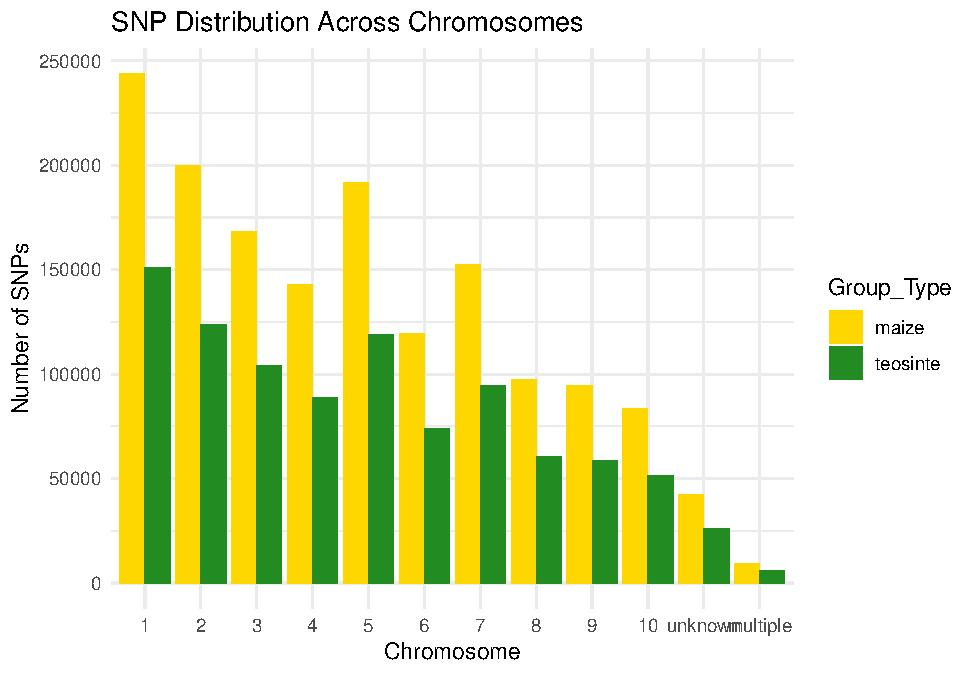
\includegraphics{R_Assignment_files/figure-latex/unnamed-chunk-11-1.pdf}

\paragraph{Distribution of SNP Across
Chromosome}\label{distribution-of-snp-across-chromosome}

\begin{Shaded}
\begin{Highlighting}[]
\FunctionTok{ggplot}\NormalTok{(joint\_snpALL\_long }\SpecialCharTok{\%\textgreater{}\%} \FunctionTok{filter}\NormalTok{(}\SpecialCharTok{!}\FunctionTok{is.na}\NormalTok{(Position)), }
       \FunctionTok{aes}\NormalTok{(}\AttributeTok{x =}\NormalTok{ Position }\SpecialCharTok{/} \FloatTok{1e6}\NormalTok{, }\AttributeTok{y =}\NormalTok{ Chromosome)) }\SpecialCharTok{+}
  \FunctionTok{geom\_bin2d}\NormalTok{(}\AttributeTok{bins =} \DecValTok{100}\NormalTok{) }\SpecialCharTok{+}  
  \FunctionTok{scale\_fill\_viridis\_c}\NormalTok{() }\SpecialCharTok{+} 
  \FunctionTok{labs}\NormalTok{(}\AttributeTok{title =} \StringTok{"SNP Density Along Chromosomes"}\NormalTok{,}
       \AttributeTok{x =} \StringTok{"Position (Mb)"}\NormalTok{, }\AttributeTok{y =} \StringTok{"Chromosome"}\NormalTok{, }\AttributeTok{fill =} \StringTok{"Density"}\NormalTok{) }\SpecialCharTok{+}
  \FunctionTok{theme\_minimal}\NormalTok{()}
\end{Highlighting}
\end{Shaded}

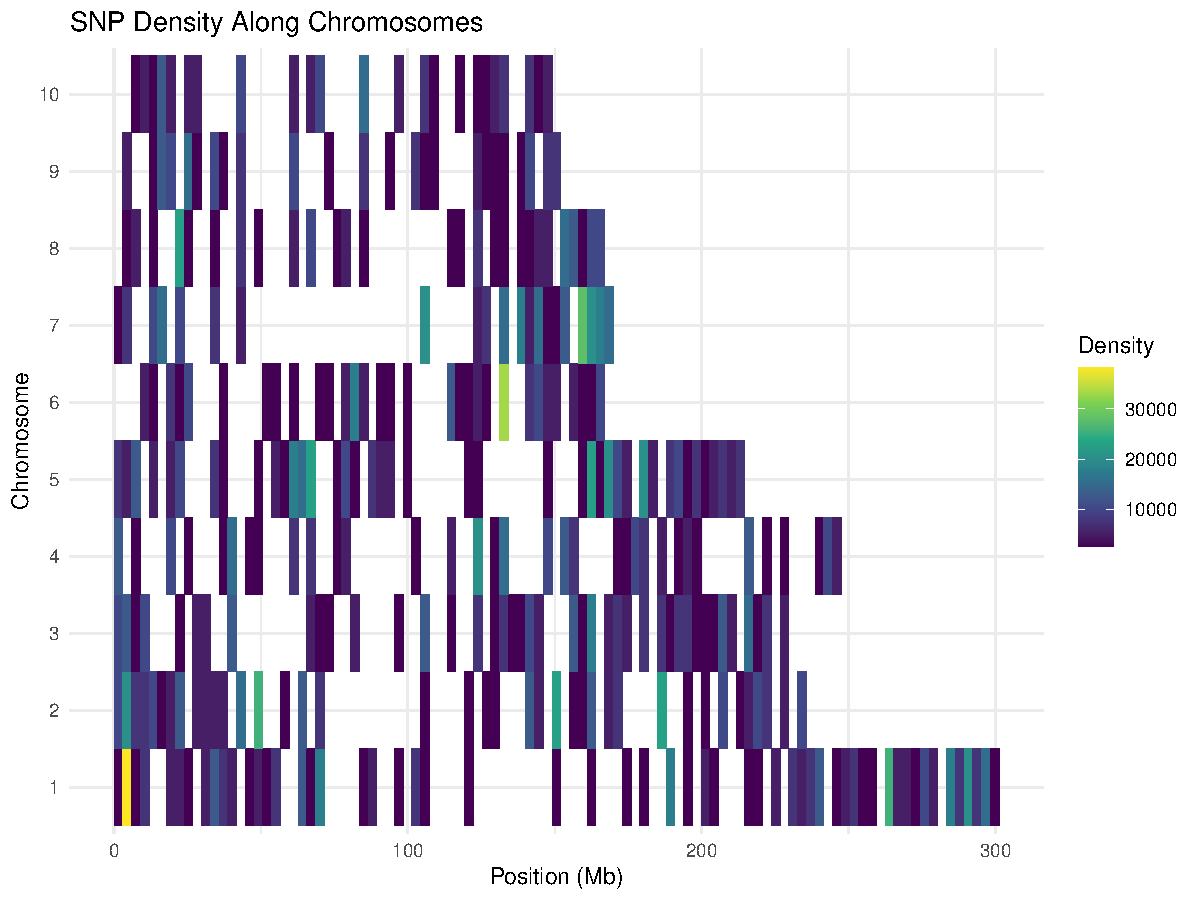
\includegraphics{R_Assignment_files/figure-latex/unnamed-chunk-12-1.pdf}

\subsubsection{Missing data and amount of
heterozygosity}\label{missing-data-and-amount-of-heterozygosity}

\begin{Shaded}
\begin{Highlighting}[]
\NormalTok{genotype\_summary }\OtherTok{\textless{}{-}}\NormalTok{ joint\_snpALL\_long }\SpecialCharTok{\%\textgreater{}\%}
  \FunctionTok{mutate}\NormalTok{(}\AttributeTok{Genotype\_Class =} \FunctionTok{case\_when}\NormalTok{(}
\NormalTok{    Genotype }\SpecialCharTok{==} \StringTok{"?/?"} \SpecialCharTok{\textasciitilde{}} \StringTok{"missing"}\NormalTok{,}
    \FunctionTok{substr}\NormalTok{(Genotype, }\DecValTok{1}\NormalTok{, }\DecValTok{1}\NormalTok{) }\SpecialCharTok{==} \FunctionTok{substr}\NormalTok{(Genotype, }\DecValTok{3}\NormalTok{, }\DecValTok{3}\NormalTok{) }\SpecialCharTok{\textasciitilde{}} \StringTok{"homozygous"}\NormalTok{,}
    \ConstantTok{TRUE} \SpecialCharTok{\textasciitilde{}} \StringTok{"heterozygous"}
\NormalTok{  )) }\SpecialCharTok{\%\textgreater{}\%}
  \FunctionTok{count}\NormalTok{(Sample\_ID, Group, Genotype\_Class) }\SpecialCharTok{\%\textgreater{}\%}
  \FunctionTok{group\_by}\NormalTok{(Sample\_ID, Group) }\SpecialCharTok{\%\textgreater{}\%}
  \FunctionTok{mutate}\NormalTok{(}\AttributeTok{Proportion =}\NormalTok{ n }\SpecialCharTok{/} \FunctionTok{sum}\NormalTok{(n))}

\FunctionTok{ggplot}\NormalTok{(genotype\_summary, }\FunctionTok{aes}\NormalTok{(}\AttributeTok{x =} \FunctionTok{reorder}\NormalTok{(Sample\_ID, }\SpecialCharTok{{-}}\NormalTok{Proportion, }\AttributeTok{FUN =}\NormalTok{ sum), }
                             \AttributeTok{y =}\NormalTok{ Proportion, }\AttributeTok{fill =}\NormalTok{ Genotype\_Class)) }\SpecialCharTok{+}
  \FunctionTok{geom\_col}\NormalTok{(}\AttributeTok{position =} \StringTok{"stack"}\NormalTok{, }\AttributeTok{width =} \FloatTok{0.8}\NormalTok{) }\SpecialCharTok{+}
  \FunctionTok{scale\_fill\_manual}\NormalTok{(}\AttributeTok{values =} \FunctionTok{c}\NormalTok{(}\StringTok{"homozygous"} \OtherTok{=} \StringTok{"\#2E86C1"}\NormalTok{, }
                               \StringTok{"heterozygous"} \OtherTok{=} \StringTok{"\#28B463"}\NormalTok{,  }
                               \StringTok{"missing"} \OtherTok{=} \StringTok{"\#E74C3C"}\NormalTok{)) }\SpecialCharTok{+}
  \FunctionTok{labs}\NormalTok{(}\AttributeTok{title =} \StringTok{"Proportion of Genotypes per Sample"}\NormalTok{,}
       \AttributeTok{subtitle =} \StringTok{"Grouped by Maize and Teosinte"}\NormalTok{,}
       \AttributeTok{x =} \StringTok{"Sample ID"}\NormalTok{, }\AttributeTok{y =} \StringTok{"Proportion"}\NormalTok{, }\AttributeTok{fill =} \StringTok{"Genotype Type"}\NormalTok{) }\SpecialCharTok{+}
  \FunctionTok{facet\_wrap}\NormalTok{(}\SpecialCharTok{\textasciitilde{}}\NormalTok{ Group, }\AttributeTok{scales =} \StringTok{"free\_x"}\NormalTok{) }\SpecialCharTok{+}
  \FunctionTok{theme\_minimal}\NormalTok{(}\AttributeTok{base\_size =} \DecValTok{14}\NormalTok{) }\SpecialCharTok{+}
  \FunctionTok{theme}\NormalTok{(}
    \AttributeTok{plot.title =} \FunctionTok{element\_text}\NormalTok{(}\AttributeTok{face =} \StringTok{"bold"}\NormalTok{, }\AttributeTok{size =} \DecValTok{18}\NormalTok{, }\AttributeTok{hjust =} \FloatTok{0.5}\NormalTok{),  }
    \AttributeTok{plot.subtitle =} \FunctionTok{element\_text}\NormalTok{(}\AttributeTok{size =} \DecValTok{14}\NormalTok{, }\AttributeTok{hjust =} \FloatTok{0.5}\NormalTok{, }\AttributeTok{color =} \StringTok{"gray50"}\NormalTok{),  }
    \AttributeTok{axis.title =} \FunctionTok{element\_text}\NormalTok{(}\AttributeTok{size =} \DecValTok{14}\NormalTok{, }\AttributeTok{face =} \StringTok{"bold"}\NormalTok{),  }
    \AttributeTok{axis.text.x =} \FunctionTok{element\_blank}\NormalTok{(),  }
    \AttributeTok{axis.ticks.x =} \FunctionTok{element\_blank}\NormalTok{(),  }
    \AttributeTok{panel.grid.major.x =} \FunctionTok{element\_blank}\NormalTok{(),  }
    \AttributeTok{panel.grid.minor =} \FunctionTok{element\_blank}\NormalTok{(),  }
    \AttributeTok{legend.position =} \StringTok{"top"}\NormalTok{,  }
    \AttributeTok{legend.title =} \FunctionTok{element\_text}\NormalTok{(}\AttributeTok{face =} \StringTok{"bold"}\NormalTok{),  }
    \AttributeTok{legend.key.size =} \FunctionTok{unit}\NormalTok{(}\FloatTok{0.8}\NormalTok{, }\StringTok{"cm"}\NormalTok{)  }
\NormalTok{  ) }\SpecialCharTok{+}
  \FunctionTok{guides}\NormalTok{(}\AttributeTok{fill =} \FunctionTok{guide\_legend}\NormalTok{(}\AttributeTok{title =} \StringTok{"Genotype Class"}\NormalTok{))}
\end{Highlighting}
\end{Shaded}

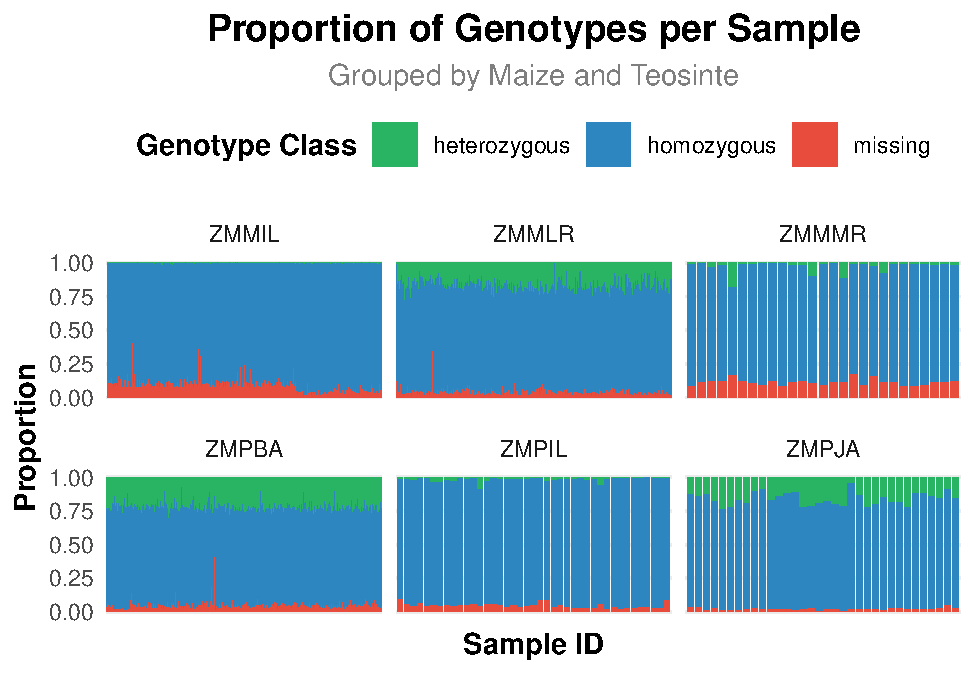
\includegraphics{R_Assignment_files/figure-latex/unnamed-chunk-13-1.pdf}

\subsubsection{My own visualization}\label{my-own-visualization}

\paragraph{Genotype Distribution Across
Chromosomes}\label{genotype-distribution-across-chromosomes}

\begin{Shaded}
\begin{Highlighting}[]
\NormalTok{chromosome\_genotype }\OtherTok{\textless{}{-}}\NormalTok{ joint\_snpALL\_long }\SpecialCharTok{\%\textgreater{}\%}
  \FunctionTok{mutate}\NormalTok{(}\AttributeTok{Genotype\_Class =} \FunctionTok{case\_when}\NormalTok{(}
\NormalTok{    Genotype }\SpecialCharTok{==} \StringTok{"?/?"} \SpecialCharTok{\textasciitilde{}} \StringTok{"missing"}\NormalTok{,}
    \FunctionTok{substr}\NormalTok{(Genotype, }\DecValTok{1}\NormalTok{, }\DecValTok{1}\NormalTok{) }\SpecialCharTok{==} \FunctionTok{substr}\NormalTok{(Genotype, }\DecValTok{3}\NormalTok{, }\DecValTok{3}\NormalTok{) }\SpecialCharTok{\textasciitilde{}} \StringTok{"homozygous"}\NormalTok{,}
    \ConstantTok{TRUE} \SpecialCharTok{\textasciitilde{}} \StringTok{"heterozygous"}
\NormalTok{  )) }\SpecialCharTok{\%\textgreater{}\%}
  \FunctionTok{group\_by}\NormalTok{(Chromosome, Genotype\_Class) }\SpecialCharTok{\%\textgreater{}\%}
  \FunctionTok{summarise}\NormalTok{(}\AttributeTok{Count =} \FunctionTok{n}\NormalTok{(), }\AttributeTok{.groups =} \StringTok{"drop"}\NormalTok{)}

\FunctionTok{ggplot}\NormalTok{(chromosome\_genotype, }\FunctionTok{aes}\NormalTok{(}\AttributeTok{x =} \FunctionTok{factor}\NormalTok{(Chromosome, }\AttributeTok{levels =} \FunctionTok{sort}\NormalTok{(}\FunctionTok{unique}\NormalTok{(Chromosome))), }
                                \AttributeTok{y =}\NormalTok{ Count, }\AttributeTok{fill =}\NormalTok{ Genotype\_Class)) }\SpecialCharTok{+}
  \FunctionTok{geom\_bar}\NormalTok{(}\AttributeTok{stat =} \StringTok{"identity"}\NormalTok{, }\AttributeTok{position =} \StringTok{"fill"}\NormalTok{) }\SpecialCharTok{+}  
  \FunctionTok{scale\_fill\_manual}\NormalTok{(}\AttributeTok{values =} \FunctionTok{c}\NormalTok{(}\StringTok{"homozygous"} \OtherTok{=} \StringTok{"\#2E86C1"}\NormalTok{, }\StringTok{"heterozygous"} \OtherTok{=} \StringTok{"\#28B463"}\NormalTok{, }\StringTok{"missing"} \OtherTok{=} \StringTok{"\#E74C3C"}\NormalTok{)) }\SpecialCharTok{+}
  \FunctionTok{labs}\NormalTok{(}\AttributeTok{title =} \StringTok{"Genotype Type Distribution Across Chromosomes"}\NormalTok{,}
       \AttributeTok{x =} \StringTok{"Chromosome"}\NormalTok{, }\AttributeTok{y =} \StringTok{"Proportion"}\NormalTok{, }\AttributeTok{fill =} \StringTok{"Genotype Type"}\NormalTok{) }\SpecialCharTok{+}
  \FunctionTok{theme\_minimal}\NormalTok{()}
\end{Highlighting}
\end{Shaded}

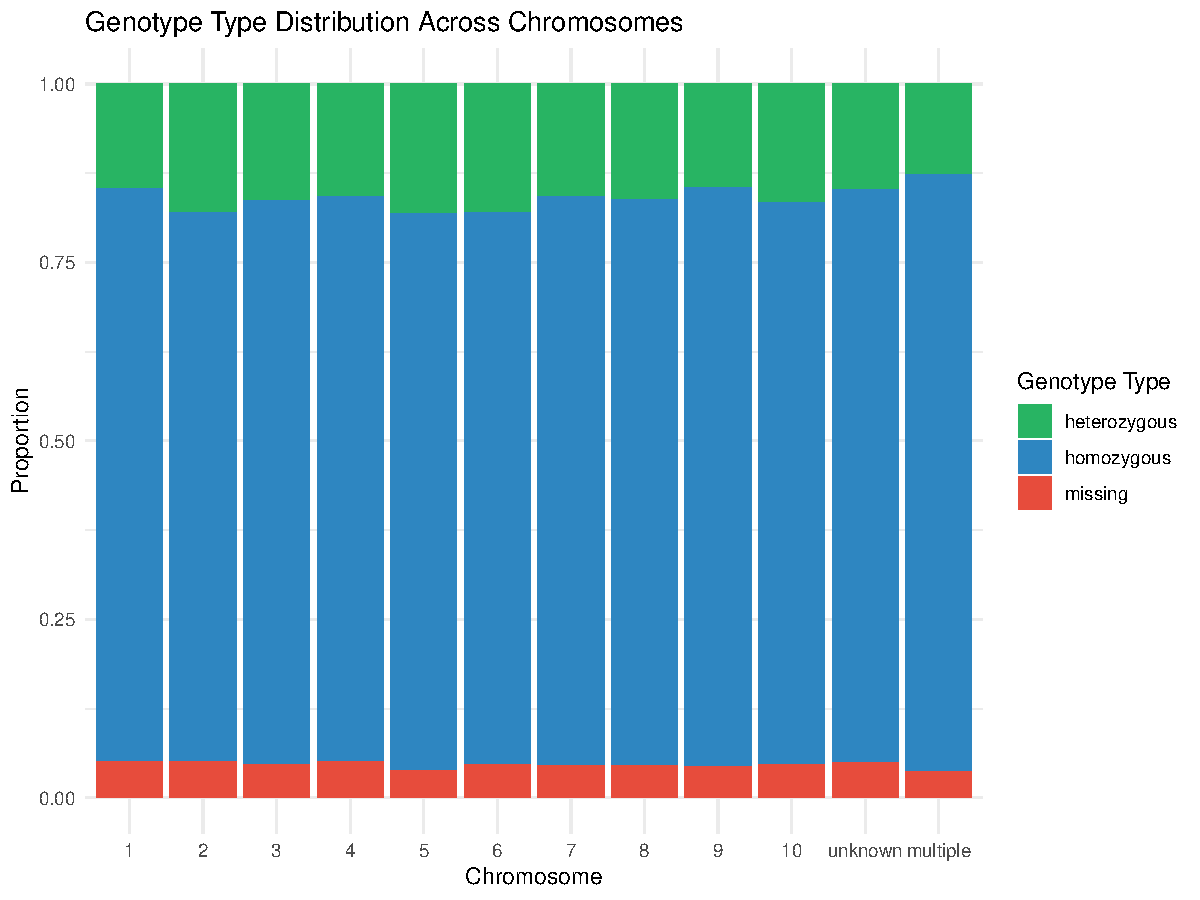
\includegraphics{R_Assignment_files/figure-latex/unnamed-chunk-14-1.pdf}

\end{document}
